\documentclass[11pt,a4paper]{report}
\usepackage[T1]{fontenc}
\usepackage{lmodern}
\usepackage[english]{babel}
\usepackage[margin=22mm]{geometry}
\usepackage{amsmath,amssymb,booktabs,longtable,array,xcolor,graphicx,float}
\usepackage{tikz}
\usetikzlibrary{arrows.meta,positioning,fit,backgrounds}
\usepackage{fvextra}
\usepackage{hyperref}
\hypersetup{colorlinks=true,linkcolor=blue!55!black,urlcolor=teal!60!black,pdftitle={SM4 controlled DFA: code, execution and full key recovery},pdfauthor={Guilherme Martins Specht}}
\fvset{fontsize=\scriptsize,breaklines=true,breakanywhere=true,numbers=left,numbersep=4pt,xleftmargin=5mm}
\setlength{\emergencystretch}{3em}
\setcounter{tocdepth}{1}
\newcommand{\hx}[1]{\texttt{#1}}
\newcommand{\xor}{\mathbin{\oplus}}
\newcommand{\rol}{\operatorname{rol}}
\newcommand{\remember}[1]{\par\medskip\noindent\fcolorbox{teal!60!black}{teal!3}{\parbox{\dimexpr\linewidth-2\fboxsep-2\fboxrule\relax}{#1}}\par\medskip}
\tikzset{box/.style={draw,rounded corners,align=center,minimum height=11mm,text width=36mm,fill=blue!4},smallbox/.style={draw,align=center,minimum width=28mm,minimum height=10mm},flow/.style={-{Stealth},thick},fault/.style={draw=red!70!black,fill=red!6,text=red!70!black}}
\begin{document}
\hypersetup{pageanchor=false}
\begin{titlepage}
\centering
\vspace*{15mm}
{\Large Polytech Montpellier --- PFE 5A\par}
\vspace{12mm}
{\Huge\bfseries Understanding SM4 Fault-Based Key Recovery\par}
\vspace{8mm}
{\LARGE A line-by-line illustrated execution guide to\par}
\vspace{3mm}
{\Large\texttt{piret\_sm4.py} and \texttt{run.py}\par}
\vspace{15mm}
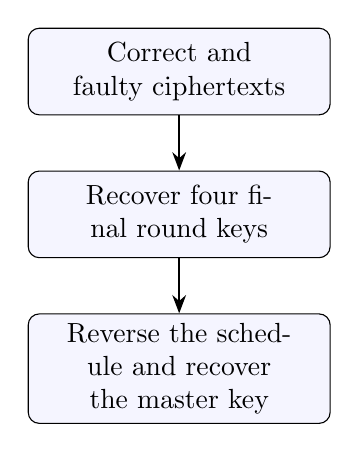
\begin{tikzpicture}
\node[box] (c) {Correct and faulty ciphertexts};
\node[box,below=7mm of c] (k) {Recover four final round keys};
\node[box,below=7mm of k] (m) {Reverse the schedule and recover the master key};
\draw[flow] (c)--(k);\draw[flow] (k)--(m);
\end{tikzpicture}
\vfill
{\large Guilherme Martins Specht\par}
\vspace{3mm}
Academic supervisor: Prof. Philippe Maurine\par
Industrial collaboration: STMicroelectronics\par
\vspace{8mm}
Independent educational document --- 8 November 2026\par
\end{titlepage}
\pagenumbering{roman}
\hypersetup{pageanchor=true}
\tableofcontents
\clearpage
\pagenumbering{arabic}

\chapter{What this lesson demonstrates}
\section{The question we will answer}
How can a program recover an unknown SM4 master key by comparing correct and faulty ciphertexts? We will follow one complete execution, connect each equation to the Python code, and explain why every recovered byte is justified by observations.

This document is independent of the main AES/SM4 report. It includes its own explanations, drawings, numerical tables and current-code excerpts. All generated numerical tables come from an actual execution of the implementation, not manually invented intermediate values.

\remember{\textbf{Precise scope.} The module is named \texttt{piret\_sm4.py}, but the experiment is a controlled-byte SM4 DFA extension. It is not the AES Piret attack applied unchanged. The model assumes a known XOR mask at a selected S-box input byte in each of rounds 31, 30, 29 and 28. Physical glitch access with these properties has not been demonstrated here.}

\section{Run exactly this experiment}
From the repository root:
\begin{Verbatim}[numbers=none]
python src/run.py --algorithm sm4 --step
\end{Verbatim}
The equivalent attack-specific entry point is:
\begin{Verbatim}[numbers=none]
python src/piret_sm4.py --step
\end{Verbatim}
The former calls \texttt{run.main()} and then \texttt{sm4\_demo()}. The latter parses its arguments and calls the same \texttt{run.sm4\_demo()}. The mathematical lesson is shared; log filenames differ.

Press Enter at a teaching pause. A stage can contain hundreds of printed candidate tests: scroll within the terminal before continuing. Remove \texttt{--step} to execute continuously. The default limit is eight observations \emph{per target byte}; it is not eight faults for the entire recovery.

The worked vector is fixed:
\begin{Verbatim}[numbers=none]
Plaintext:  0123456789ABCDEFFEDCBA9876543210
Master key: 0123456789ABCDEFFEDCBA9876543210
Ciphertext: 681EDF34D206965E86B3E94F536E4246
\end{Verbatim}
Interactive defaults come from \texttt{sm4.KEY} and \texttt{sm4.PLAINTEXT}. If you change them, the equations still apply but the printed numbers change. The document generator deliberately uses the fixed public vector above.

\section{Separate what the target knows from what the attacker knows}
\begin{center}
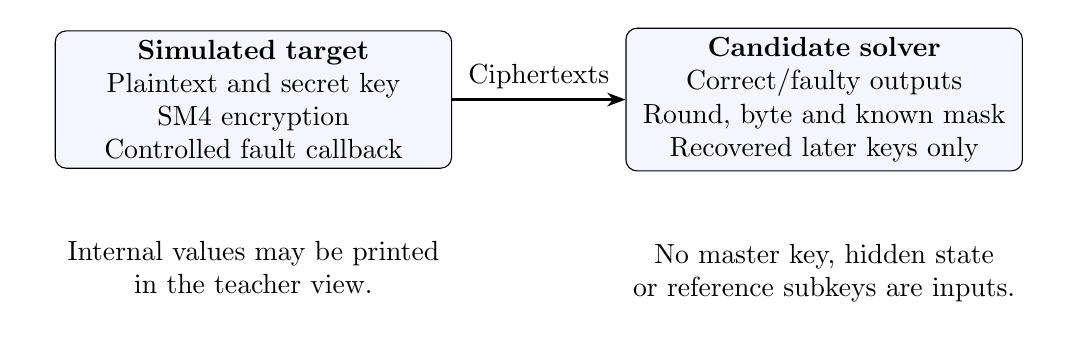
\begin{tikzpicture}
\node[box,text width=48mm] (target) {\textbf{Simulated target}\\Plaintext and secret key\\SM4 encryption\\Controlled fault callback};
\node[box,text width=48mm,right=22mm of target] (solver) {\textbf{Candidate solver}\\Correct/faulty outputs\\Round, byte and known mask\\Recovered later keys only};
\draw[flow] (target)--node[above,align=center]{Ciphertexts}(solver);
\node[below=8mm of target,align=center,text width=55mm] {Internal values may be printed\\in the teacher view.};
\node[below=8mm of solver,align=center,text width=55mm] {No master key, hidden state\\or reference subkeys are inputs.};
\end{tikzpicture}
\end{center}
\texttt{oracle(round, byte, mask)} is a callable that requests a faulty encryption. It represents an experimental target interface, not a cryptographic oracle that reveals the key. In this simulation the callback closes over the target key; its return value is only a ciphertext.

\section{A map of the files}
\begin{center}\begin{tabular}{p{42mm}p{105mm}}\toprule
File&Responsibility\\\midrule
\texttt{sm4.py}&Normal SM4 encryption, decryption and generic observation hooks.\\
\texttt{piret\_sm4.py}&Fault adapter, inverse diffusion, candidate equations, round peeling, recovery and inverse schedule.\\
\texttt{run.py}&Terminal orchestration, comparisons, pauses, observation reporting and final checks.\\
\texttt{attack\_steps.py}&Detailed numerical teaching events used by terminal and GUI.\\
\texttt{terminal\_log.py}&Mirror execution to the terminal, TXT and colored HTML logs.\\\bottomrule
\end{tabular}\end{center}

\chapter{Read the SM4 round before attacking it}
\section{Bytes, words and numbering}
One byte is eight bits. One SM4 word is four bytes, or 32 bits. A block contains four words, or 16 bytes. Word byte order is big-endian: byte 0 is the leftmost, most significant byte.
Byte and word values in the worked cryptographic calculations are hexadecimal; round numbers and bit indices are decimal.
\begin{center}
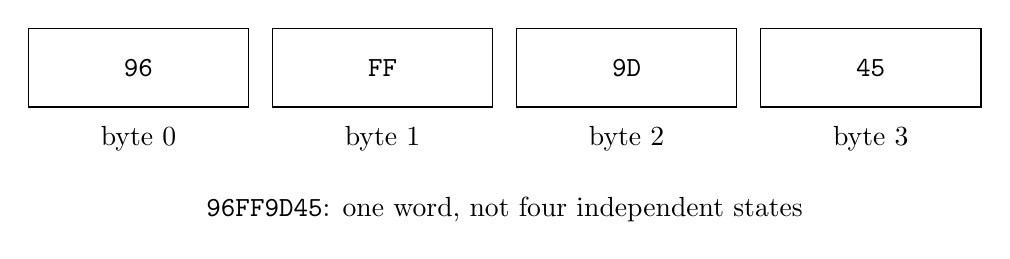
\begin{tikzpicture}
\foreach \v/\p in {96/0,FF/1,9D/2,45/3}{\node[smallbox] at (\p*3.1,0) {\texttt{\v}};\node at (\p*3.1,-.9) {byte \p};}
\node[align=center] at (4.65,-1.8) {\texttt{96FF9D45}: one word, not four independent states};
\end{tikzpicture}
\end{center}
Round indices are zero-based: round 31 is the \emph{32nd} and final round. SM4 creates words \(X_4,\ldots,X_{35}\). The final ciphertext is
\[C=X_{35}\parallel X_{34}\parallel X_{33}\parallel X_{32}.\]
Word reversal is not byte reversal within each word.

\section{Four calculations form one round}
For round \(i\):
\begin{align*}
A&=X_{i+1}\xor X_{i+2}\xor X_{i+3}\xor rk_i,\\
B&=\tau(A),\\
D&=L(B)=B\xor\rol(B,2)\xor\rol(B,10)\xor\rol(B,18)\xor\rol(B,24),\\
X_{i+4}&=X_i\xor D.
\end{align*}
The four bytes pass independently through the SM4 S-box in \(\tau\). The rotations in \(L\) mix bits across the word. All rotations operate on 32 bits and wrap around.
\begin{center}
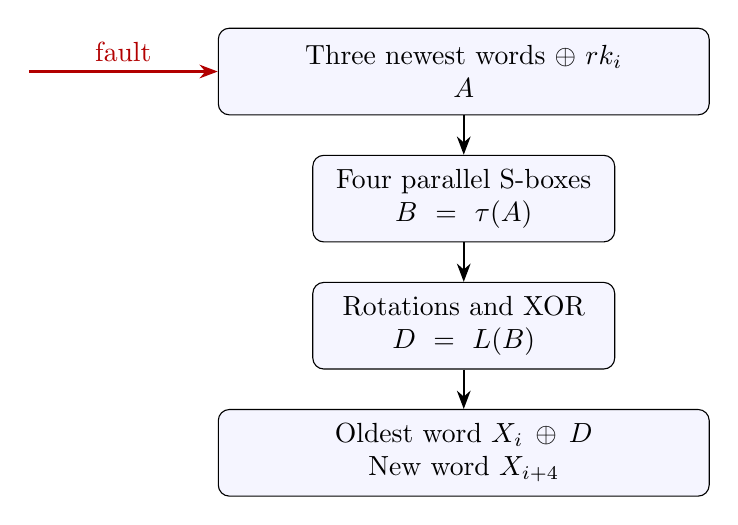
\begin{tikzpicture}[node distance=5mm]
\node[box,text width=60mm] (a) {Three newest words $\xor\ rk_i$\\$A$};
\node[box,below=of a] (b) {Four parallel S-boxes\\$B=\tau(A)$};
\node[box,below=of b] (l) {Rotations and XOR\\$D=L(B)$};
\node[box,below=of l,text width=60mm] (x) {Oldest word $X_i\xor D$\\New word $X_{i+4}$};
\draw[flow](a)--(b);\draw[flow](b)--(l);\draw[flow](l)--(x);
\draw[flow,red!70!black] ([xshift=-24mm]a.west)--node[above]{fault}(a.west);
\end{tikzpicture}
\end{center}

\section{Translate the normal terminal line}
\begin{Verbatim}[numbers=none]
Round 00: A=F002C39E B=18E992B1 L(B)=26D99622 new=27FAD345
\end{Verbatim}
\texttt{run.sm4\_demo()} first obtains the clean trace with \texttt{sm4\_encrypt()}, a wrapper around the target adapter with no selected fault byte. The \texttt{for item in trace} loop prints one record per round. A record is a dictionary: \texttt{item['a']} is the S-box input; \texttt{item['new']} is the new word.

\texttt{sm4.round()} calls \texttt{observe()} around each intermediate value. Without an observer, a value is returned unchanged. With a callback, returning \texttt{None} preserves it; returning an integer replaces it. This separates a normal cipher from attack-specific interventions.

\section{The last clean round of our example}
\begin{align*}
X_{31}&=\hx{7B938F4C},&rk_{31}&=\hx{9124A012},\\
A&=\hx{96FF9D45},&B&=\hx{1A488C73},\\
L(B)&=\hx{138D5078},&X_{35}&=\hx{681EDF34}.
\end{align*}
Check the last equation:
\[\hx{7B938F4C}\xor\hx{138D5078}=\hx{681EDF34}.\]
These internal values are shown to verify the simulation. The solver must recover \(rk_{31}\), not take it from this display. All 32 clean-round records are reproduced in Appendix A.

\chapter{Follow the Python call chain}
\section{Who calls whom?}
\begin{center}
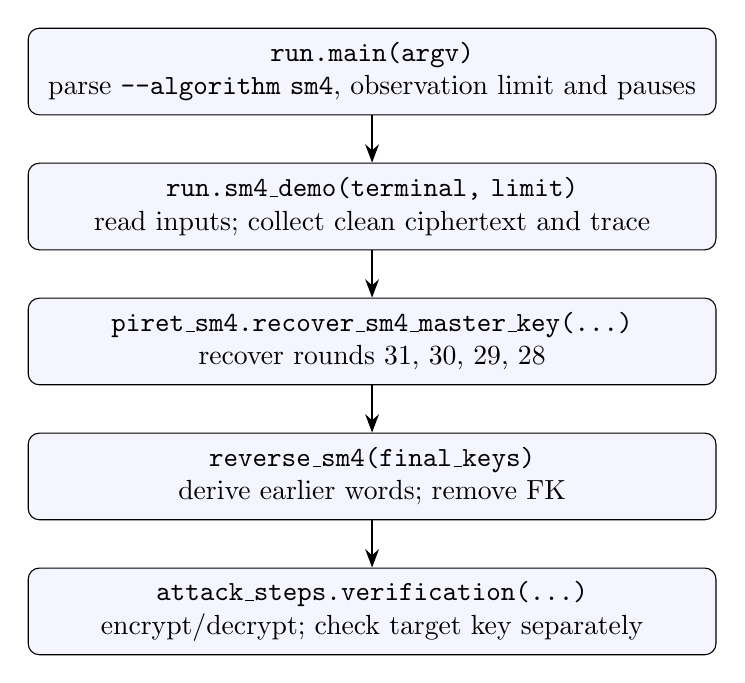
\begin{tikzpicture}[node distance=6mm]
\node[box,text width=85mm] (main) {\texttt{run.main(argv)}\\parse \texttt{--algorithm sm4}, observation limit and pauses};
\node[box,below=of main,text width=85mm] (demo) {\texttt{run.sm4\_demo(terminal, limit)}\\read inputs; collect clean ciphertext and trace};
\node[box,below=of demo,text width=85mm] (recover) {\texttt{piret\_sm4.recover\_sm4\_master\_key(...)}\\recover rounds 31, 30, 29, 28};
\node[box,below=of recover,text width=85mm] (schedule) {\texttt{reverse\_sm4(final\_keys)}\\derive earlier words; remove FK};
\node[box,below=of schedule,text width=85mm] (verify) {\texttt{attack\_steps.verification(...)}\\encrypt/decrypt; check target key separately};
\draw[flow](main)--(demo);\draw[flow](demo)--(recover);\draw[flow](recover)--(schedule);\draw[flow](schedule)--(verify);
\end{tikzpicture}
\end{center}
The detailed presentation may reverse the schedule again to print every numerical step. That repetition is a consistency check of the display, not a second independent key recovery or an additional fault query.

\section{The two nested callbacks in \texttt{sm4\_demo}}
\begin{Verbatim}
def oracle(number, byte, mask):
    faulty, fault_trace = piret_sm4.sm4_fault_encrypt(plaintext, key, byte, mask, number)
    # Teacher-only propagation is displayed here.
    return faulty

def report(event):
    show_sm4_observation(terminal, event, recovered_bytes, start_byte)
\end{Verbatim}
This shortened excerpt omits only the teacher-printing call. The complete current function is included in the source appendix. These are nested functions: they can read the surrounding \texttt{plaintext}, \texttt{key} and \texttt{terminal}. Only the oracle accesses the target key. The report callback receives copied observation metadata after the solver has computed the intersection.

\texttt{range(1, limit+1)} supplies masks \(01,02,\ldots\) up to the requested maximum. Although the first two masks each flip one bit, this controlled-byte model permits other nonzero byte masks, including multi-bit masks. The program stops early whenever a byte becomes unique.

\section{What data is stored?}
\begin{center}\begin{tabular}{p{35mm}p{112mm}}\toprule
Variable&Meaning\\\midrule
\texttt{keys}&Dictionary of already recovered round keys; initially empty.\\
\texttt{subkey}&Four-byte buffer for the current round key.\\
\texttt{survivors}&Set of compatible key-byte values. \texttt{None} means no observation yet.\\
\texttt{fresh}&Candidates compatible with only the current ciphertext pair.\\
\texttt{history}&Observation dictionaries used by logs and GUI explanations.\\
\texttt{used}&Number of actual faulty ciphertext queries.\\
\texttt{clean\_view}&Ciphertext-style four-word view restored to the target round.\\
\texttt{faulty\_view}&Equivalent restored view for the faulty encryption.\\\bottomrule
\end{tabular}\end{center}

\chapter{First fault: recover candidates for byte 0 of rk31}
\section{Step 1: the external callback changes one byte}
The relevant line in \texttt{sm4\_fault\_encrypt()} is:
\begin{Verbatim}
if number == fault_round and operation == "Sbox input" and byte is not None:
    value ^= mask << (24 - 8 * byte)
\end{Verbatim}
The three conditions select the round, intermediate value and whether a fault was requested. \texttt{byte=None} creates a clean run. For \texttt{byte=0}, the shift is 24, so mask \texttt{01} becomes \texttt{01000000}. The augmented assignment \texttt{\^{}=} XORs the mask into the current 32-bit value.
\[\hx{96FF9D45}\xor\hx{01000000}=\hx{97FF9D45}.\]
The observer returns the changed value to the actual SM4 round. Its trace stores \texttt{a}, \texttt{b}, \texttt{linear} and \texttt{new} for teaching.

\section{Step 2: the S-box changes the difference}
For the selected input byte:
\[S(\hx{96})=\hx{1A},\qquad S(\hx{97})=\hx{55}.\]
Therefore
\[\Delta B=\hx{1A488C73}\xor\hx{55488C73}=\hx{4F000000}.\]
\begin{center}
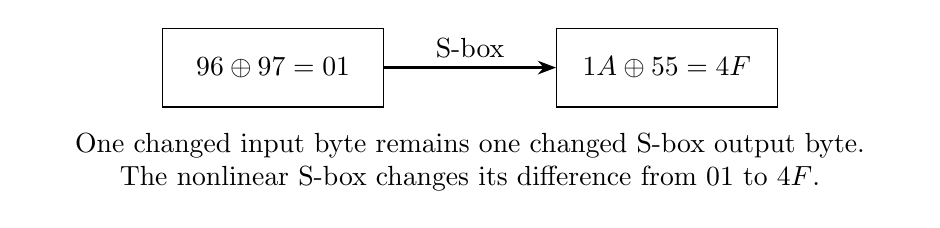
\begin{tikzpicture}
\node[smallbox] (a) at (0,0) {$96\xor97=01$};
\node[smallbox] (b) at (5,0) {$1A\xor55=4F$};
\draw[flow] (a)--node[above]{S-box}(b);
\node[align=center,text width=110mm] at (2.5,-1.2) {One changed input byte remains one changed S-box output byte.\\The nonlinear S-box changes its difference from $01$ to $4F$.};
\end{tikzpicture}
\end{center}

\section{Step 3: linear diffusion spreads that byte difference}
\[L(\hx{4F000000})=\hx{734E3D3D}.\]
The four bytes are now nonzero. Since the oldest input word remains unchanged, this is also the newest output-word difference:
\[X'_{35}=\hx{681EDF34}\xor\hx{734E3D3D}=\hx{1B50E209}.\]
\begin{center}
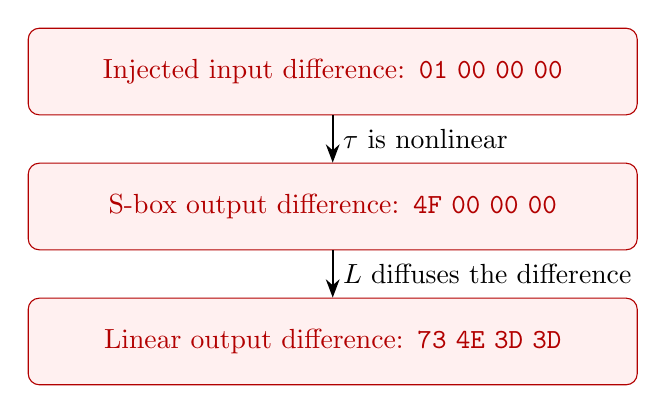
\begin{tikzpicture}[node distance=6mm]
\node[box,fault,text width=75mm] (in) {Injected input difference: \texttt{01 00 00 00}};
\node[box,fault,below=of in,text width=75mm] (sb) {S-box output difference: \texttt{4F 00 00 00}};
\node[box,fault,below=of sb,text width=75mm] (lin) {Linear output difference: \texttt{73 4E 3D 3D}};
\draw[flow](in)--node[right]{$\tau$ is nonlinear}(sb);
\draw[flow](sb)--node[right]{$L$ diffuses the difference}(lin);
\end{tikzpicture}
\end{center}
\remember{\textbf{Why does the teacher-view XOR contain many bytes?} Its four displayed words are \(A\), \(\tau(A)\), \(L(\tau(A))\), and the new word. They are four intermediate results concatenated for display, not the complete cipher state. Only the first injected difference is a one-byte mask.}

\section{Step 4: keep only the public ciphertexts}
\begin{Verbatim}[numbers=none]
Correct: 681EDF34 D206965E 86B3E94F 536E4246
Faulty:  1B50E209 D206965E 86B3E94F 536E4246
XOR:     734E3D3D 00000000 00000000 00000000
\end{Verbatim}
\texttt{struct.unpack(">4I", ciphertext)} converts 16 bytes into four big-endian unsigned words. The solver checks \texttt{c[1:] == f[1:]}. If any of those three unchanged words differs, this pair does not satisfy the assumed restored last-round model and is rejected.

\section{Step 5: derive the equation that cancels the hidden old word}
The two last-round equations are:
\[X_{35}=X_{31}\xor L(B),\qquad X'_{35}=X_{31}\xor L(B').\]
XORing them cancels \(X_{31}\) because a value XORed with itself is zero:
\begin{align*}
\Delta X&=X_{35}\xor X'_{35}\\
&=X_{31}\xor X_{31}\xor L(B)\xor L(B')\\
&=L(B\xor B')=L(\Delta B).
\end{align*}
So the attacker can compute \(\Delta B=L^{-1}(\Delta X)\) without knowing \(X_{31}\), \(B\), \(B'\) or the round key.

\chapter{Understand inverse L without treating it as magic}
\section{What does GF(2) mean here?}
GF(2) contains only 0 and 1. Addition is XOR and multiplication is AND. In particular \(1+1=0\). A 32-bit word can be treated as a vector of 32 such coefficients.

Rotations rearrange bit positions. XOR combines them. Thus \(L(u\xor v)=L(u)\xor L(v)\), and L can be represented by a binary matrix \(M\):
\[\Delta X=M\Delta B,\qquad\Delta B=M^{-1}\Delta X.\]
Here arithmetic is bitwise GF(2), not the AES byte-field multiplication in GF(\(2^8\)).

\section{How \texttt{inverse\_rows()} constructs the inverse}
\begin{enumerate}
\item For each bit position \(i\), compute \texttt{sm4.linear(1 << i)}. This gives column \(i\) of M.
\item Assemble 32 rows and append an identity matrix: \([M\mid I]\).
\item For each column, select a pivot row containing a 1 and swap it into place.
\item XOR that row into every other row having a 1 in the same column.
\item The left half becomes I, and the right half becomes \(M^{-1}\).
\end{enumerate}
There is no division: the only nonzero pivot in GF(2) is 1. The implementation packs each augmented row into a Python integer; the lower 32 bits store M and the upper 32 bits store I. After elimination, \texttt{row >> 32} extracts an inverse row. \texttt{@lru\_cache(maxsize=1)} caches this public, key-independent matrix.

\section{A smaller four-bit drawing of the same method}
This is a toy matrix, \emph{not} the SM4 matrix, so we can see the entire operation:
\[
\left[\begin{array}{cccc|cccc}
1&1&0&0&1&0&0&0\\0&1&1&0&0&1&0&0\\0&0&1&1&0&0&1&0\\0&0&0&1&0&0&0&1
\end{array}\right]
\longrightarrow
\left[\begin{array}{cccc|cccc}
1&0&0&0&1&1&1&1\\0&1&0&0&0&1&1&1\\0&0&1&0&0&0&1&1\\0&0&0&1&0&0&0&1
\end{array}\right].
\]
The toy matrix maps \(1010\) to \(1110\); the right-hand inverse maps \(1110\) back to \(1010\). The real code performs the same kind of elimination with 32 rows.

\section{Two equivalent ways the code applies the inverse}
The solver's expanded \texttt{inverse\_linear(value)} calculates a dot product for each inverse row in explicit steps:
\begin{Verbatim}
selected_bits = row & value
set_bit_count = bin(selected_bits).count("1")
parity = set_bit_count & 1
result |= parity << index
\end{Verbatim}
\texttt{row \& value} selects shared set bits. Counting them and keeping the lowest bit computes parity: an even count gives 0, an odd count gives 1. Shifting that parity to its output position and ORing disjoint bit positions assembles the word.

The detailed terminal instead explains the equivalent column/basis expansion:
\[L^{-1}(v)=\mathop{\bigoplus}_{i:v_i=1}L^{-1}(2^i).\]
It prints all 32 input-bit contributions. \texttt{inverse basis} is \(L^{-1}(2^i)\); \texttt{contribution} is that value if the input bit is 1, or zero otherwise. \texttt{running XOR} is the accumulated answer. Bit 0 is the rightmost, least significant bit.

For our example the first three relevant calculations are:
\begin{align*}
i=0:&\quad 0\xor\hx{41455115}=\hx{41455115},\\
i=1:&\quad\hx{41455115}\xor0=\hx{41455115},\\
i=2:&\quad\hx{41455115}\xor\hx{05154455}=\hx{44501540}.
\end{align*}
After all bits:
\[\boxed{L^{-1}(\hx{734E3D3D})=\hx{4F000000}}.\]
The terminal checks \(L(\hx{4F000000})=\hx{734E3D3D}\). Appendix C prints every contribution.

\chapter{Turn a difference into a recovered key byte}
\section{Select the affected byte and compute q}
For byte 0, \texttt{shift = 24 - 8*byte} equals 24. Right shifting \(\Delta B\) by 24 and masking with 255 selects \(d=\hx{4F}\). The code rejects differences with nonzero bits outside that byte.

The S-box input is
\[A=X_{32}\xor X_{33}\xor X_{34}\xor rk_{31}.\]
The three data words are visible in the ciphertext. Their XOR is:
\[\hx{D206965E}\xor\hx{86B3E94F}\xor\hx{536E4246}=\hx{07DB3D57}.\]
Its first byte is \(q=\hx{07}\). If the unknown first S-box input byte is \(a\), then
\[a=q\xor k,\qquad \boxed{k=a\xor q}.\]
\remember{The solver guesses the unknown \emph{S-box input} \(a\) first. It converts compatible inputs into key-byte guesses using q. The variable \texttt{inputs} is therefore not the same set as the returned key-byte candidates.}

\section{First observation: two inputs remain}
For known mask \(e=\hx{01}\), try every \(a=00,\ldots,FF\):
\[S(a)\xor S(a\xor\hx{01})=\hx{4F}.\]
Only \(a=\hx{96}\) and \(a=\hx{97}\) pass. For instance:
\[S(\hx{96})\xor S(\hx{97})=\hx{1A}\xor\hx{55}=\hx{4F}.\]
The order can be reversed and the XOR stays the same, explaining this pair of inputs. Convert them to key guesses:
\[\hx{96}\xor\hx{07}=\hx{91},\qquad\hx{97}\xor\hx{07}=\hx{90}.\]
So the first key-byte set is \(\{\hx{90},\hx{91}\}\). Even though the teacher view showed input \(96\), the solver must not use that hidden value to discard \(90\).

\section{Second observation: intersect, do not guess}
Request a new fault at the \emph{same} byte with mask \(02\). The faulty ciphertext is
\begin{Verbatim}[numbers=none]
ED9DD932 D206965E 86B3E94F 536E4246
\end{Verbatim}
The recovered S-box difference is \(\hx{81000000}\), giving \(d=\hx{81}\). The compatible inputs are:
\[\{\hx{75},\hx{77},\hx{94},\hx{96}\}.\]
After XOR with \(q=07\), the fresh key guesses are:
\[\{\hx{70},\hx{72},\hx{91},\hx{93}\}.\]
Intersect with the first observation:
\[\boxed{\{90,91\}\cap\{70,72,91,93\}=\{91\}}.\]
\begin{center}
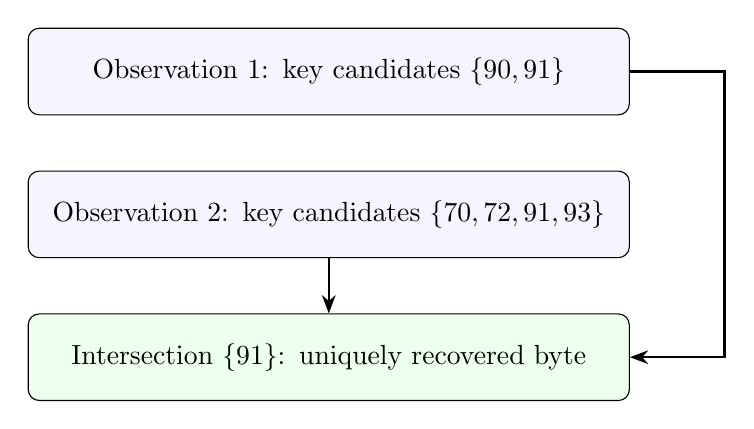
\begin{tikzpicture}[node distance=7mm]
\node[box,text width=74mm] (first) {Observation 1: key candidates $\{90,91\}$};
\node[box,below=of first,text width=74mm] (second) {Observation 2: key candidates $\{70,72,91,93\}$};
\node[box,below=of second,text width=74mm,fill=green!7] (unique) {Intersection $\{91\}$: uniquely recovered byte};
\draw[flow](first.east)--++(12mm,0)|-(unique.east);
\draw[flow](second)--(unique);
\end{tikzpicture}
\end{center}
The terminal prints \texttt{RECOVERED rk31 byte 0 = 91 / UNIQUE}. Full input tests for both observations are in Appendix D.

\section{Understand the recovery loop and Python's for--else}
The essential blocks in \texttt{recover\_sm4\_master\_key()} are:
\begin{Verbatim}
survivors = None
for observation, mask in enumerate(masks, 1):
    faulty = bytes(fault_oracle(number, byte, mask))
    faulty_view = peel_sm4(faulty, number, keys)
    fresh, inputs, delta = sm4_byte_candidates(clean_view, faulty_view, byte, mask)
    if survivors is None:
        survivors = set(fresh)
    else:
        survivors = survivors & fresh
    if not survivors:
        raise ValueError(...)
    if len(survivors) == 1:
        subkey[byte] = next(iter(survivors))
        break
else:
    return ...  # incomplete result, with master_key=None
\end{Verbatim}
This is an explanatory excerpt: event creation and the optional alternative filter are omitted here but preserved in the full source appendix.
\begin{itemize}
\item \texttt{enumerate(masks,1)} gives a human-readable observation count starting at 1.
\item \texttt{None} means no constraint yet; an empty set means inconsistent observations.
\item \texttt{\&} intersects sets. It does not perform byte XOR.
\item \texttt{next(iter(survivors))} is safe here only because the length was checked to be exactly one.
\item \texttt{break} stops querying this byte once it is unique.
\item The \texttt{else} belongs to the \emph{for loop}, not the preceding if: it runs only if the loop ends without a break. An ambiguous byte blocks full recovery.
\end{itemize}

\chapter{Recover all four tail keys, not just rk31}
\section{Finish the other bytes of rk31}
The same equations recover bytes 1, 2 and 3. Their q bytes are \(DB,3D,57\), respectively. They become \(24,A0,12\). Concatenate in big-endian order:
\[rk_{31}=\hx{91}\parallel\hx{24}\parallel\hx{A0}\parallel\hx{12}=\hx{9124A012}.\]
\texttt{int.from\_bytes(subkey,"big")} performs this assembly. Four unique bytes are required before \texttt{keys[31]} is populated.

\section{Why do we need new faults in earlier rounds?}
One 32-bit subkey does not supply the four consecutive words required to invert SM4's 128-bit key schedule. Recover the final four subkeys in reverse chronological order:
\begin{center}
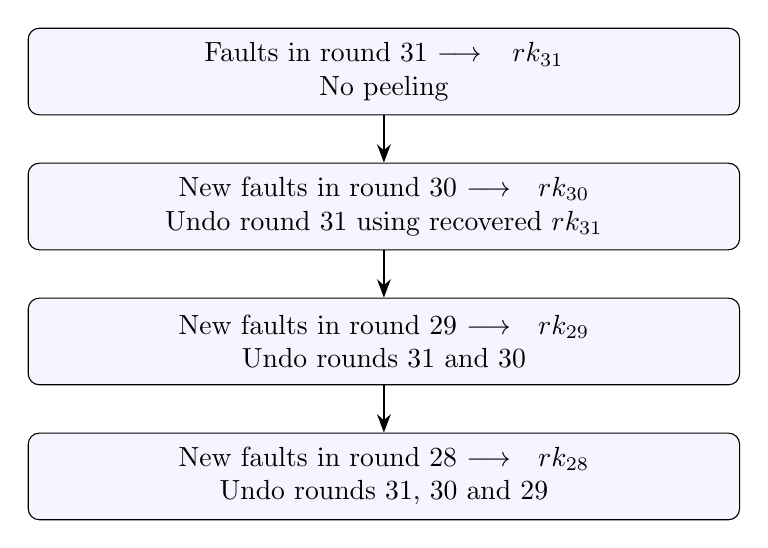
\begin{tikzpicture}[node distance=6mm]
\node[box,text width=88mm] (r31) {Faults in round 31 $\longrightarrow rk_{31}$\\No peeling};
\node[box,below=of r31,text width=88mm] (r30) {New faults in round 30 $\longrightarrow rk_{30}$\\Undo round 31 using recovered $rk_{31}$};
\node[box,below=of r30,text width=88mm] (r29) {New faults in round 29 $\longrightarrow rk_{29}$\\Undo rounds 31 and 30};
\node[box,below=of r29,text width=88mm] (r28) {New faults in round 28 $\longrightarrow rk_{28}$\\Undo rounds 31, 30 and 29};
\draw[flow](r31)--(r30);\draw[flow](r30)--(r29);\draw[flow](r29)--(r28);
\end{tikzpicture}
\end{center}
The program does not reuse a last-round faulty ciphertext and pretend it reveals earlier keys. It requests a new target encryption at each selected earlier round.

\section{How \texttt{peel\_sm4()} restores an older window}
Let the chronological post-round state be \((u_0,u_1,u_2,u_3)\). With the recovered key of that round:
\begin{align*}
A&=u_0\xor u_1\xor u_2\xor rk,\\
\text{previous}&=u_3\xor L(\tau(A)),\\
\text{restored state}&=(\text{previous},u_0,u_1,u_2).
\end{align*}
\begin{center}
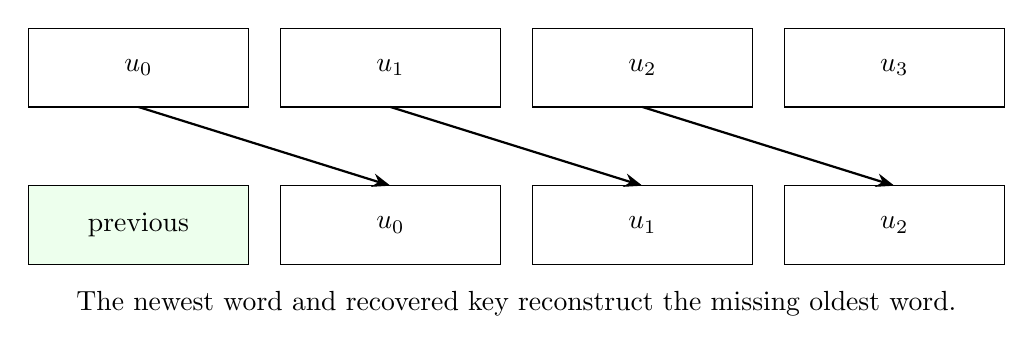
\begin{tikzpicture}
\foreach \v/\p in {u_0/0,u_1/1,u_2/2,u_3/3}{\node[smallbox] at (\p*3.2,0) {$\v$};}
\node[smallbox,fill=green!7] at (0,-2) {previous};
\foreach \v/\p in {u_0/1,u_1/2,u_2/3}{\node[smallbox] at (\p*3.2,-2) {$\v$};}
\draw[flow] (0,-.5)--(3.2,-1.5);\draw[flow](3.2,-.5)--(6.4,-1.5);\draw[flow](6.4,-.5)--(9.6,-1.5);
\node[align=center] at (4.8,-3) {The newest word and recovered key reconstruct the missing oldest word.};
\end{tikzpicture}
\end{center}
\texttt{words = unpack(...)[::-1]} restores chronological order. The loop runs only over later rounds. A missing recovered key raises an error. The function finally serializes \texttt{words[::-1]} again to preserve the ciphertext-style layout expected by the byte filter.

\section{A real round-30 example from the execution}
Below, \texttt{correct}/\texttt{faulty} are actual final ciphertexts. \texttt{clean\_view}/\texttt{faulty\_view} are synthetic restored outputs after undoing round 31. They are not a second physical measurement.
\VerbatimInput[numbers=none]{generated/peeling.txt}

After peeling, the same newest-word difference equation and unchanged-word checks apply to round 30. Repeat the process for rounds 29 and 28.

\section{Result and actual query count}
For this fixed example every byte becomes unique after two observations:
\[4\text{ target rounds}\times4\text{ bytes}\times2\text{ observations}=32\text{ faulty ciphertexts}.\]
There is also a clean reference ciphertext. Diagnostic replays and schedule printing do not increase \texttt{result['used']}.
\begin{center}\begin{tabular}{cl}\toprule Recovered key&Value\\\midrule
$rk_{31}$&\hx{9124A012}\\$rk_{30}$&\hx{01CF72E5}\\$rk_{29}$&\hx{62293496}\\$rk_{28}$&\hx{428D3654}\\\bottomrule\end{tabular}\end{center}
The count 32 is the measured result for this vector and these masks, not a universal fault requirement. Appendix B lists all 32 observations, fresh candidate sets and intersections.

\chapter{Reverse the schedule to obtain the original master key}
\section{Public CK and FK are not secret material}
The four fixed FK words are
\[\hx{A3B1BAC6},\quad\hx{56AA3350},\quad\hx{677D9197},\quad\hx{B27022DC}.\]
They initialize \(K_i=MK_i\xor FK_i\). The 32 CK words are generated from public byte values:
\[ck_{i,j}=7(4i+j)\bmod256,\qquad CK_i=ck_{i,0}\parallel\cdots\parallel ck_{i,3}.\]
For example \(CK_0=\hx{00070E15}\), \(CK_{31}=\hx{646B7279}\). FK values are directly specified constants; the implementation does not derive them from CK. Neither set depends on the secret key.

\section{Four recovered subkeys seed the inverse recurrence}
\[K_{32}=rk_{28},\quad K_{33}=rk_{29},\quad K_{34}=rk_{30},\quad K_{35}=rk_{31}.\]
The forward recurrence is
\[K_{i+4}=K_i\xor L'(\tau(K_{i+1}\xor K_{i+2}\xor K_{i+3}\xor CK_i)).\]
XOR is self-inverse, so
\[\boxed{K_i=K_{i+4}\xor L'(\tau(K_{i+1}\xor K_{i+2}\xor K_{i+3}\xor CK_i))}.\]
The code iterates \texttt{range(31,-1,-1)}: 31, 30, \ldots, 0. This order guarantees that the four required higher-index words are already known.

\section{Read one inverse schedule step}
For \(i=31\), calculate:
\[U=K_{32}\xor K_{33}\xor K_{34}\xor CK_{31}.\]
Then substitute all four bytes and apply
\[L'(B)=B\xor\rol(B,13)\xor\rol(B,23).\]
Finally compute \(K_{31}=K_{35}\xor L'(\tau(U))=\hx{F1780C81}\).
\remember{\textbf{Do not confuse the transforms.} Encryption uses rotations 2, 10, 18 and 24. Key expansion uses 13 and 23. The code correctly calls \texttt{sm4.linear\_key()}, not \texttt{sm4.linear()}, inside \texttt{reverse\_sm4()}.}

The terminal prints every S-box lookup and rotation. Earlier encryption keys \(rk_{27},\ldots,rk_0\) are labeled \texttt{DERIVED}: they come from the schedule, not additional fault observations. Appendix E contains all 32 numerical inverse steps.

\section{Remove FK and assemble the 128-bit key}
The first four recovered schedule words still contain whitening:
\[MK_i=K_i\xor FK_i\quad(i=0,1,2,3).\]
\begingroup\small
\begin{longtable}{rllll}
\toprule
$i$ & $K_i$ & $FK_i$ & $MK_i=K_i\oplus FK_i$ & Role\\
\midrule
\endfirsthead
\toprule
$i$ & $K_i$ & $FK_i$ & $MK_i=K_i\oplus FK_i$ & Role\\
\midrule
\endhead
0 & \texttt{A292FFA1} & \texttt{A3B1BAC6} & \texttt{01234567} & Master word\\
1 & \texttt{DF01FEBF} & \texttt{56AA3350} & \texttt{89ABCDEF} & Master word\\
2 & \texttt{99A12B0F} & \texttt{677D9197} & \texttt{FEDCBA98} & Master word\\
3 & \texttt{C42410CC} & \texttt{B27022DC} & \texttt{76543210} & Master word\\
\bottomrule
\end{longtable}
\endgroup

Concatenate the four 32-bit words:
\[\boxed{MK=\hx{01234567}\parallel\hx{89ABCDEF}\parallel\hx{FEDCBA98}\parallel\hx{76543210}}.\]
\texttt{struct.pack(">4I", ...)} produces the original 16 key bytes in big-endian word order.

\chapter{Final checks, logs and presentation checklist}
\section{What does PASS establish?}
The terminal independently verifies:
\begin{enumerate}
\item Encryption with the recovered key equals the original correct ciphertext.
\item Decryption of the correct ciphertext with the recovered key equals the plaintext.
\item The displayed inverse schedule agrees with the recovery engine.
\item The recovered key equals the simulated target key, revealed for ground-truth validation.
\end{enumerate}
These checks establish consistency for the executed software experiment. A correct round trip by itself would not prove that an attack had recovered the target key; the ciphertext and ground-truth comparisons matter.
\begin{Verbatim}[numbers=none]
Recovered key: 0123456789ABCDEFFEDCBA9876543210
Encrypt(P, recovered key): 681EDF34D206965E86B3E94F536E4246
Decrypt(C, recovered key): 0123456789ABCDEFFEDCBA9876543210
SM4 MASTER KEY: 0123456789ABCDEFFEDCBA9876543210 / PASS
32 faulty outputs. All four subkeys came from DFA, not references.
\end{Verbatim}
This block combines the final values for readability; exact heading wording is determined by the executable version.

\section{How the terminal explanation and logs are produced}
\texttt{show\_sm4\_observation()} calls the detailed event generator in \texttt{attack\_steps.sm4\_observation()}. It explains peeling, all inverse-L contributions and all 256 candidate inputs, then prints concise recovered-byte summaries. Seeing a summary after a detailed table is not an extra observation.

\texttt{LessonTerminal.pair()} prints correct/faulty/XOR values and colors changed bytes red. A nonzero XOR means a difference, not necessarily an additional fault. \texttt{terminal.pause()} only waits when \texttt{--step} was requested; it does not change any cryptographic values.

\texttt{run\_with\_log()} surrounds the complete entry point. The Tee objects duplicate stdout and stderr. The TXT file preserves ANSI sequences; a final HTML conversion renders red differences and green recovery results. A new execution overwrites only the same program's previous log.
\begin{center}\begin{tabular}{ll}\toprule Command entry point&Log pair\\\midrule
\texttt{run.py}&\texttt{logs/run.txt}, \texttt{logs/run.html}\\
\texttt{piret\_sm4.py}&\texttt{logs/piret\_sm4.txt}, \texttt{logs/piret\_sm4.html}\\\bottomrule\end{tabular}\end{center}

\section{Common misunderstandings to avoid}
\begin{itemize}
\item A one-byte injected error can spread across a whole word after L.
\item \(\Delta B=4F000000\) is an S-box output difference, not the mask 01 and not the key.
\item q is calculated from observable unchanged words, not read from a hidden register.
\item Multiple candidates mean ambiguity. They are not interchangeable recovered keys.
\item One recovered round key is insufficient to reverse the complete SM4 schedule.
\item Earlier-round peeling uses recovered later keys; reference keys are not solver inputs.
\item This software target accepts exact round/byte/mask requests. A physical clock or voltage glitch does not automatically provide that control.
\end{itemize}

\section{A short oral explanation}
\begin{quote}
I first run normal SM4 to obtain a reference ciphertext. I inject a known byte XOR at a selected final-round S-box input. The ciphertext XOR removes unchanged terms. Inverting the public linear transformation isolates an S-box output difference. I enumerate possible S-box inputs, convert them into key-byte guesses using public words, and intersect independent observations until one value remains. After recovering rk31, I request new faults in earlier rounds and undo only rounds whose keys are already recovered. Four consecutive recovered tail keys let me reverse the key schedule, remove FK and reconstruct the master key. Finally I verify encryption, decryption and simulation ground truth.
\end{quote}

\chapter{Connect the Python statements to a physical experiment}
\section{Three different meanings of ``execution''}
\remember{\textbf{Today: all Python functions in this lesson run on your PC.} The simulator calls \texttt{sm4.py}; it does not communicate with the ChipWhisperer or STM32. The following drawings describe how those roles would map to a future board experiment. They are conceptual diagrams, not measured waveforms or a wiring guide.}

\begin{center}
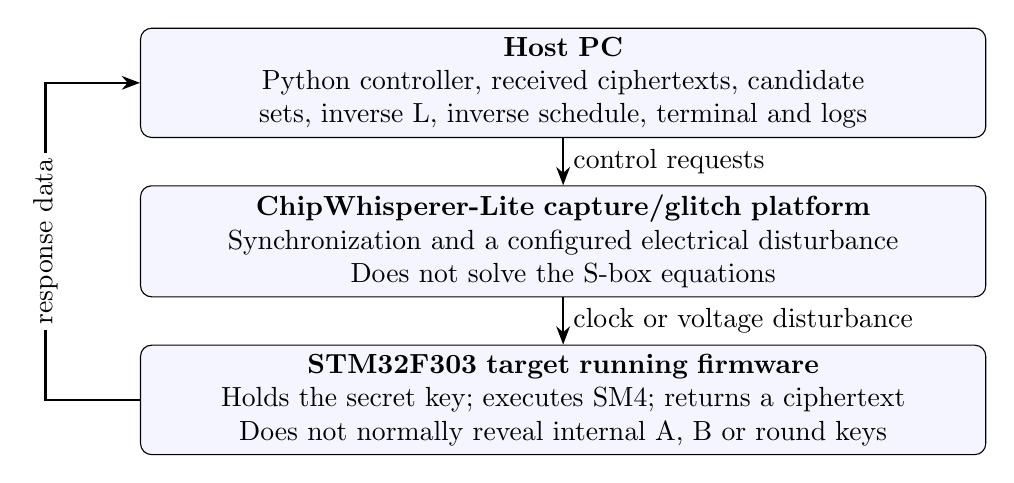
\begin{tikzpicture}[node distance=6mm]
\node[box,text width=105mm] (host) {\textbf{Host PC}\\Python controller, received ciphertexts, candidate sets, inverse L, inverse schedule, terminal and logs};
\node[box,below=of host,text width=105mm] (cw) {\textbf{ChipWhisperer-Lite capture/glitch platform}\\Synchronization and a configured electrical disturbance\\Does not solve the S-box equations};
\node[box,below=of cw,text width=105mm] (stm) {\textbf{STM32F303 target running firmware}\\Holds the secret key; executes SM4; returns a ciphertext\\Does not normally reveal internal A, B or round keys};
\draw[flow](host)--node[right]{control requests}(cw);
\draw[flow](cw)--node[right]{clock or voltage disturbance}(stm);
\draw[flow] (stm.west)--++(-12mm,0)|-(host.west);
\node[rotate=90,fill=white,inner sep=2pt] at ([xshift=-12mm]cw.west) {response data};
\end{tikzpicture}
\end{center}
The response path is schematic: an actual transport implementation determines how the host exchanges commands and bytes with the target. The current \texttt{oracle()} is a Python callable, not that transport. Clock and voltage glitching are distinct configurations; this drawing does not imply both are applied together.

\section{What happens to a word on a processor?}
In Python, \texttt{value} is an integer object in the host process. In compiled firmware, a corresponding intermediate word may be in a CPU register, stack or RAM, depending on the compiler and instructions. Without examining the firmware binary and timing, we cannot assign it to a specific physical register or clock edge.

\begin{center}
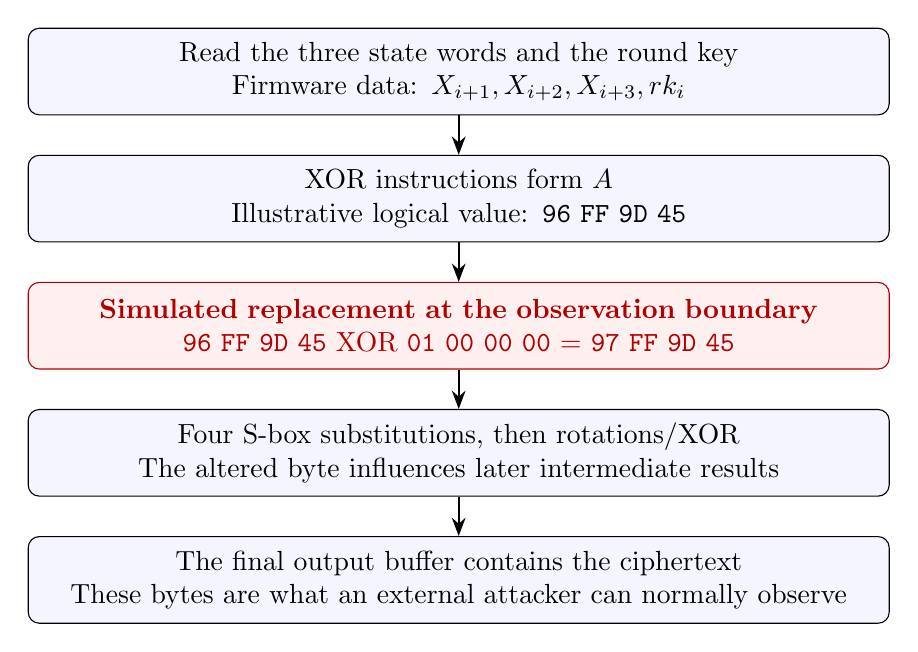
\begin{tikzpicture}[node distance=5mm]
\node[box,text width=107mm] (load) {Read the three state words and the round key\\Firmware data: $X_{i+1},X_{i+2},X_{i+3},rk_i$};
\node[box,below=of load,text width=107mm] (xor) {XOR instructions form $A$\\Illustrative logical value: \texttt{96 FF 9D 45}};
\node[box,fault,below=of xor,text width=107mm] (faultword) {\textbf{Simulated replacement at the observation boundary}\\\texttt{96 FF 9D 45} XOR \texttt{01 00 00 00} = \texttt{97 FF 9D 45}};
\node[box,below=of faultword,text width=107mm] (lookup) {Four S-box substitutions, then rotations/XOR\\The altered byte influences later intermediate results};
\node[box,below=of lookup,text width=107mm] (send) {The final output buffer contains the ciphertext\\These bytes are what an external attacker can normally observe};
\draw[flow](load)--(xor);\draw[flow](xor)--(faultword);\draw[flow](faultword)--(lookup);\draw[flow](lookup)--(send);
\end{tikzpicture}
\end{center}
The red box is exactly what \texttt{value \^{}= mask << (24 - 8 * byte)} models. A physical glitch does \emph{not} execute this Python assignment and does not inherently guarantee mask 01 or this precise intermediate boundary.

\section{A timing drawing: trigger, computation and disturbance}
The horizontal scale below is symbolic; it is not an experimentally measured timing window.
\begin{center}
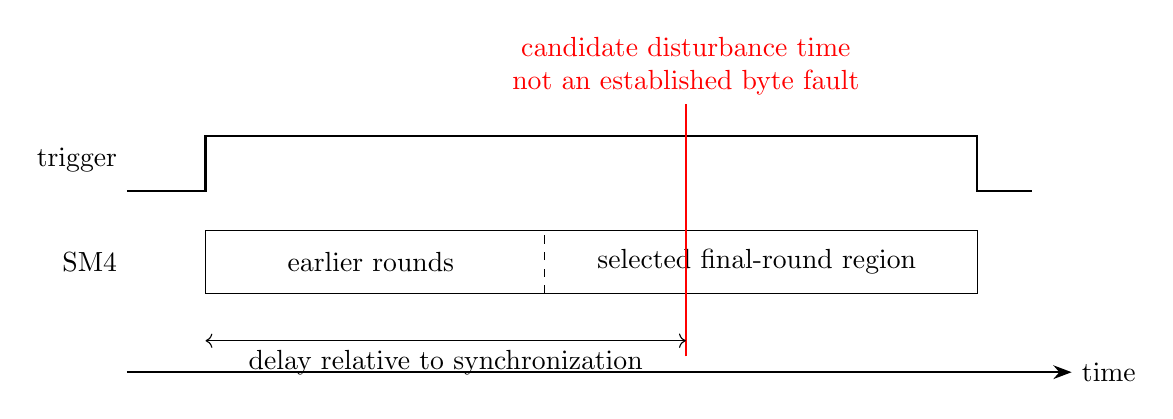
\begin{tikzpicture}[x=1cm,y=1cm]
\draw[flow] (0,0)--(12,0) node[right]{time};
\node[left] at (0,2.7) {trigger};
\draw[thick] (0,2.3)--(1,2.3)--(1,3)--(10.8,3)--(10.8,2.3)--(11.5,2.3);
\node[left] at (0,1.4) {SM4};
\draw (1,1) rectangle (10.8,1.8);
\node at (3.1,1.4) {earlier rounds};
\draw[dashed] (5.3,1)--(5.3,1.8);
\node at (8,1.4) {selected final-round region};
\draw[red,thick] (7.1,.2)--(7.1,3.4);
\node[red,above,align=center] at (7.1,3.4) {candidate disturbance time\\not an established byte fault};
\draw[<->] (1,.4)--node[below]{delay relative to synchronization}(7.1,.4);
\end{tikzpicture}
\end{center}
ChipWhisperer documentation describes trigger-synchronized glitch generation and routing for clock or voltage experiments. Whether the disturbance affects the intended operation must be characterized on the actual target. A trigger near encryption gives a time reference, not automatic knowledge of a round, byte or XOR mask.

\section{Why a physical attempt is not the same as a modeled observation}
\begin{center}
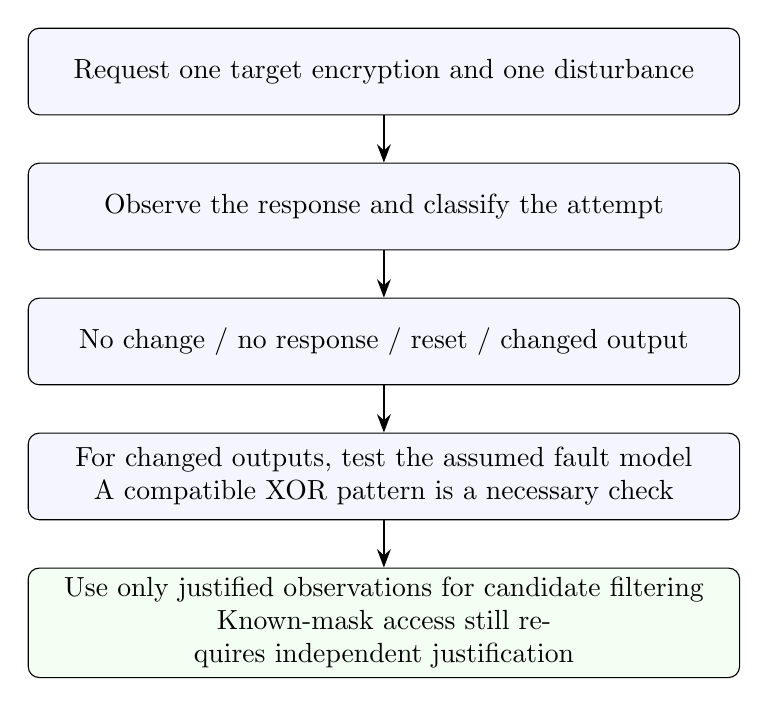
\begin{tikzpicture}[node distance=6mm]
\node[box,text width=88mm] (request) {Request one target encryption and one disturbance};
\node[box,below=of request,text width=88mm] (classify) {Observe the response and classify the attempt};
\node[box,below=of classify,text width=88mm] (cases) {No change / no response / reset / changed output};
\node[box,below=of cases,text width=88mm] (check) {For changed outputs, test the assumed fault model\\A compatible XOR pattern is a necessary check};
\node[box,below=of check,text width=88mm,fill=green!5] (solve) {Use only justified observations for candidate filtering\\Known-mask access still requires independent justification};
\draw[flow](request)--(classify);\draw[flow](classify)--(cases);\draw[flow](cases)--(check);\draw[flow](check)--(solve);
\end{tikzpicture}
\end{center}
The software model directly produces the selected byte XOR, so its \texttt{used=32} counts successful modeled ciphertext queries. A physical campaign must also count ineffective attempts, resets, rejected faults and acquisition failures. Its total attempt count is not established by the software value 32.

An output pattern consistent with a model does not by itself prove the precise physical fault location or known mask. Do not use the secret test key to select observations and then claim the attacker knew the mask independently.

\section{The candidate set exists on the PC, not inside the chip}
\begin{center}
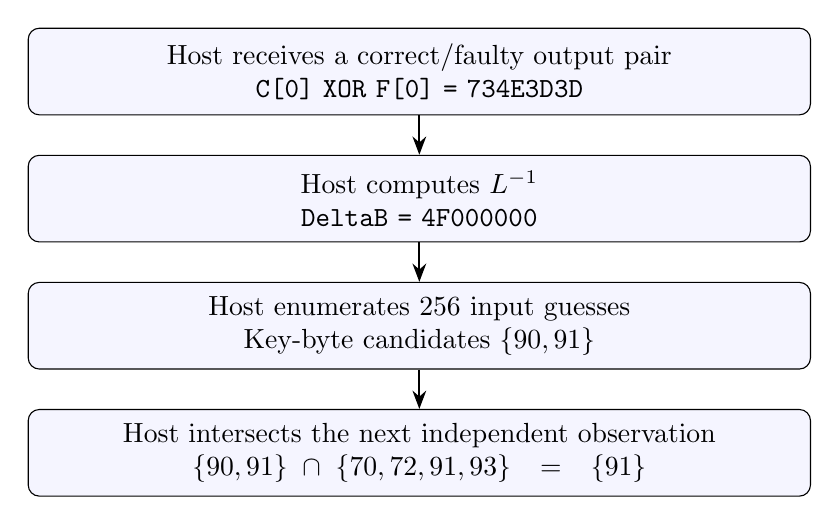
\begin{tikzpicture}[node distance=5mm]
\node[box,text width=97mm] (pair) {Host receives a correct/faulty output pair\\\texttt{C[0] XOR F[0] = 734E3D3D}};
\node[box,below=of pair,text width=97mm] (inverse) {Host computes $L^{-1}$\\\texttt{DeltaB = 4F000000}};
\node[box,below=of inverse,text width=97mm] (first) {Host enumerates 256 input guesses\\Key-byte candidates $\{90,91\}$};
\node[box,below=of first,text width=97mm] (intersection) {Host intersects the next independent observation\\$\{90,91\}\cap\{70,72,91,93\}=\{91\}$};
\draw[flow](pair)--(inverse);\draw[flow](inverse)--(first);\draw[flow](first)--(intersection);
\end{tikzpicture}
\end{center}
No operation in this drawing rewinds the target, reads its secret memory or removes bits electrically. The host is solving equations about bytes it already received.

\section{Source for the physical-platform concepts}
The hardware-role and synchronization discussion follows NewAE's official training material, \href{https://github.com/newaetech/chipwhisperer-tutorials/blob/master/courses_fault101_SOLN_Fault%201_1%20-%20Introduction%20to%20Clock%20Glitching-OPENADC-CWLITEARM.rst}{Fault 1.1: Introduction to Clock Glitching} and \href{https://github.com/newaetech/chipwhisperer-tutorials/blob/master/courses_fault101_SOLN_Fault%202_1%20-%20Introduction%20to%20Voltage%20Glitching-OPENADC-CWLITEARM.rst}{Fault 2.1: Introduction to Voltage Glitching}. Those tutorials illustrate platform concepts; their example target behavior does not validate this SM4 byte-fault model on an STM32F303.

\chapter{How to read the function-by-function pages}
The following two chapters cover \emph{every function defined in \texttt{piret\_sm4.py} and \texttt{run.py}}, including nested callbacks and methods defined in the latter's terminal class. The AES-only functions in \texttt{run.py} are explicitly labeled as inactive for \texttt{--algorithm sm4}; they are included so no function in either requested file is silently skipped.

For each function, read in this order:
\begin{enumerate}
\item The purpose sentence and its input--processing--output diagram.
\item The physical-interpretation box, which says what happens on the PC and what only models target behavior.
\item The complete numbered source, copied from the current repository.
\item The line table, explaining each executable physical source line and every continuation or alternate branch.
\end{enumerate}
Blank lines, comments and docstrings remain visible in the numbered source but have no separate execution step; the table does not pretend they perform computations. A function definition creates a callable, and a nested callback body runs later only when called. Loops cause a source line to execute repeatedly; they are not new source lines on each iteration.

The line tables describe what each statement does, not one CPU instruction per Python line. A Python expression can execute many host operations; compiled STM32 firmware has a different instruction stream. Current source line numbers and the table's coverage manifest are refreshed whenever this PDF is rebuilt.

\chapter{Line-by-line: \texttt{piret\_sm4.py}}
\section{\texttt{sm4\_fault\_encrypt}}
Simulate a controlled fault during the real SM4 implementation, while collecting teacher-only intermediates.
\begin{center}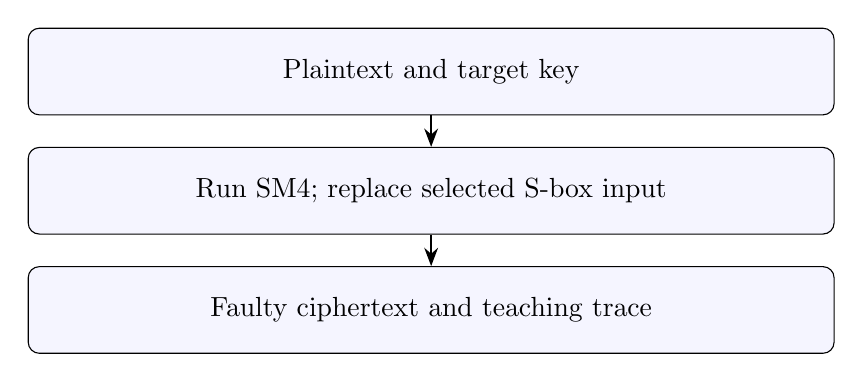
\begin{tikzpicture}[node distance=4mm]
\node[box,text width=100mm] (input) {Plaintext and target key};
\node[box,below=of input,text width=100mm] (action) {Run SM4; replace selected S-box input};
\node[box,below=of action,text width=100mm] (output) {Faulty ciphertext and teaching trace};
\draw[flow](input)--(action);\draw[flow](action)--(output);
\end{tikzpicture}\end{center}
\remember{\textbf{Physical interpretation:} Target-side behavior is modeled here. In firmware, intermediate words could occupy CPU registers or RAM depending on compilation; this Python callback does not access STM32 registers.}
\subsection*{Exact source}
\VerbatimInput[firstnumber=14]{generated/annotated_piret_sm4_sm4_fault_encrypt.txt}
\subsection*{Read each executable line}
\begingroup\small\begin{longtable}{r >{\raggedright\arraybackslash}p{138mm}}\toprule Line&Meaning and effect\\\midrule\endfirsthead\toprule Line&Meaning and effect\\\midrule\endhead
14&Declare this callable and its parameters; the body runs only when called. Simulate a controlled fault during the real SM4 implementation, while collecting teacher-only intermediates.\\
21&If a fault was requested, require a byte position 0..3 and a nonzero one-byte mask. None permits a clean reference run.\\
22&Stop this path with the stated exception. The message identifies the violated input, model or verification condition; no recovered key is accepted by this line.\\
24&Reject a selected round outside the zero-based 0..31 interval.\\
25&Stop this path with the stated exception. The message identifies the violated input, model or verification condition; no recovered key is accepted by this line.\\
28&Compute the target schedule for trace labeling. The result is a list indexed 0..31, not a dictionary; it is not passed to the output-only solver.\\
31&Create an empty teaching trace; the following explicit loop adds one record for each round.\\
33&Visit all thirty-two round indices to construct the trace records.\\
34&Add the record for this round and its target-side round key to the teacher trace.\\
36&Translate cipher callback event names into short trace dictionary fields a, b, linear and new.\\
38&Define the target callback; its body executes later when the normal cipher calls the observation hook, not when this definition is reached.\\
41&Inject only when both round and operation match, and a target byte was selected; other events pass through unchanged.\\
42&Move the mask into the selected big-endian byte and XOR it into the word. For byte 0 and mask 01, the shifted mask is 01000000.\\
44&Record only named scalar intermediate events; ignore other observation events for this teacher trace.\\
45&Save the observed scalar at its round and semantic field, so the terminal can compare clean and faulty calculations.\\
47&Return the unchanged or injected scalar to the normal SM4 engine; this returned replacement is what the next cipher operation consumes.\\
49&Execute normal SM4 with the external observer attached. A returned observer replacement is consumed by the real round function.\\
51&Return the target output together with teacher-only intermediate records. The oracle later forwards only the ciphertext to the solver.\\
\bottomrule\end{longtable}\endgroup
\section{\texttt{inverse\_rows}}
Construct and cache the inverse of the public 32-bit diffusion map.
\begin{center}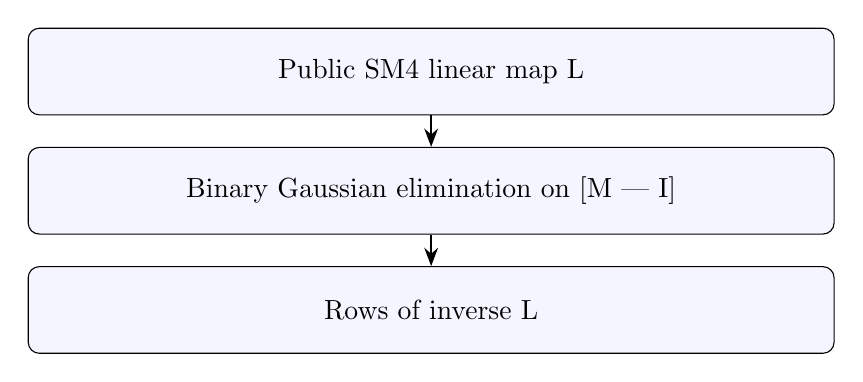
\begin{tikzpicture}[node distance=4mm]
\node[box,text width=100mm] (input) {Public SM4 linear map L};
\node[box,below=of input,text width=100mm] (action) {Binary Gaussian elimination on [M | I]};
\node[box,below=of action,text width=100mm] (output) {Rows of inverse L};
\draw[flow](input)--(action);\draw[flow](action)--(output);
\end{tikzpicture}\end{center}
\remember{\textbf{Physical interpretation:} This is attacker-side algebra on the PC. No pulse, board read or secret key is required.}
\subsection*{Exact source}
\VerbatimInput[firstnumber=54]{generated/annotated_piret_sm4_inverse_rows.txt}
\subsection*{Read each executable line}
\begingroup\small\begin{longtable}{r >{\raggedright\arraybackslash}p{138mm}}\toprule Line&Meaning and effect\\\midrule\endfirsthead\toprule Line&Meaning and effect\\\midrule\endhead
54&Cache the public inverse-matrix result after the first calculation. The matrix is key-independent and is not recomputed for every observation.\\
55&Declare this callable and its parameters; the body runs only when called. Construct and cache the inverse of the public 32-bit diffusion map.\\
59&Prepare the list of images of the thirty-two input basis words under the public map L.\\
61&Choose each input basis bit explicitly, from bit zero through bit thirty-one.\\
62&Construct a 32-bit word with exactly the selected input bit set.\\
64&Apply public encryption diffusion L to that basis word, obtaining one matrix column.\\
66&Store this basis image as the next column of the binary matrix.\\
69&Prepare the augmented-matrix row list before encoding individual row bits.\\
71&Construct each output row of the binary matrix explicitly.\\
72&Start this encoded matrix row with every bit cleared.\\
74&Read the selected output bit from each stored matrix column.\\
75&Extract the bit indicating whether this input column contributes to the selected output row.\\
76&Place that contribution bit in the encoded matrix row; OR combines disjoint bit positions.\\
78&Place the matching identity-matrix bit in the upper half of the augmented row.\\
80&Combine the L-matrix row with its identity bit to form the packed row of [M | I].\\
82&Store the completed augmented row before Gaussian elimination.\\
84&Process one pivot column of the 32-by-32 binary matrix at a time.\\
86&Mark the pivot as not yet found; the following ordinary loop searches eligible rows.\\
88&Search the current and remaining rows for a one in the pivot column.\\
89&Read the current candidate row bit at the pivot column.\\
91&Accept this row as a valid pivot only if its selected column bit is one.\\
92&Remember the actual row index, then stop searching because a valid pivot was found.\\
93&Stop searching pivot rows as soon as a valid row has been found.\\
95&Detect a missing pivot instead of blindly swapping an invalid row index.\\
96&Stop this path with the stated exception. The message identifies the violated input, model or verification condition; no recovered key is accepted by this line.\\
98&Swap the chosen pivot row into the current diagonal position.\\
100&Visit every augmented row so the current column can be cleared outside its pivot.\\
101&Leave the pivot unchanged; eliminate only another row whose pivot-column bit is one.\\
103&XOR the entire augmented pivot row into that row, performing GF(2) row elimination on both halves.\\
106&Prepare the final public inverse-matrix rows after elimination.\\
108&Visit each reduced augmented row to extract its inverse half.\\
109&Discard the lower identity half and retain the upper inverse-matrix row.\\
111&Add the extracted inverse row in the original output-bit order.\\
113&Return an immutable sequence of inverse rows, cached for reuse by later observations.\\
\bottomrule\end{longtable}\endgroup
\section{\texttt{inverse\_linear}}
Apply the inverse binary matrix to one observed output difference.
\begin{center}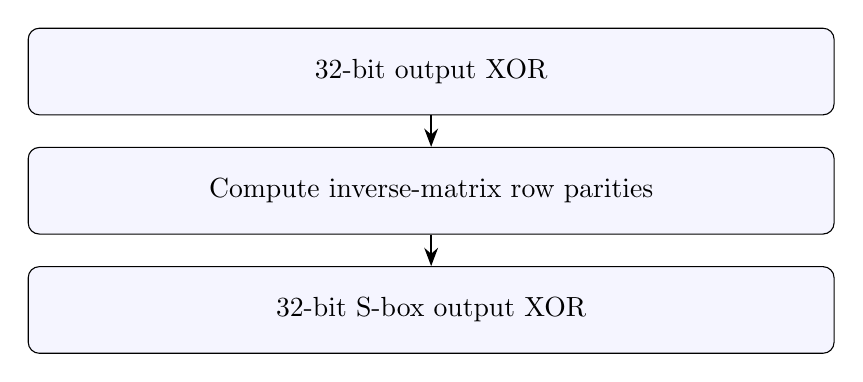
\begin{tikzpicture}[node distance=4mm]
\node[box,text width=100mm] (input) {32-bit output XOR};
\node[box,below=of input,text width=100mm] (action) {Compute inverse-matrix row parities};
\node[box,below=of action,text width=100mm] (output) {32-bit S-box output XOR};
\draw[flow](input)--(action);\draw[flow](action)--(output);
\end{tikzpicture}\end{center}
\remember{\textbf{Physical interpretation:} The PC transforms received ciphertext bytes into a mathematical difference. The target does not run backward.}
\subsection*{Exact source}
\VerbatimInput[firstnumber=116]{generated/annotated_piret_sm4_inverse_linear.txt}
\subsection*{Read each executable line}
\begingroup\small\begin{longtable}{r >{\raggedright\arraybackslash}p{138mm}}\toprule Line&Meaning and effect\\\midrule\endfirsthead\toprule Line&Meaning and effect\\\midrule\endhead
116&Declare this callable and its parameters; the body runs only when called. Apply the inverse binary matrix to one observed output difference.\\
119&Clear the output word before placing one parity bit at a time.\\
121&Associate each inverse-matrix row with the output bit it computes.\\
122&Select exactly the input bits used by this inverse row.\\
124&Count selected one bits; only whether this count is odd or even matters over GF(2).\\
126&Keep the lowest count bit: odd becomes one and even becomes zero.\\
128&Place this row parity into its output position without changing other output bits.\\
130&Return the word assembled from all thirty-two inverse-row parity calculations.\\
\bottomrule\end{longtable}\endgroup
\section{\texttt{sm4\_byte\_candidates}}
Find key-byte guesses consistent with one restored ciphertext pair and a known byte fault.
\begin{center}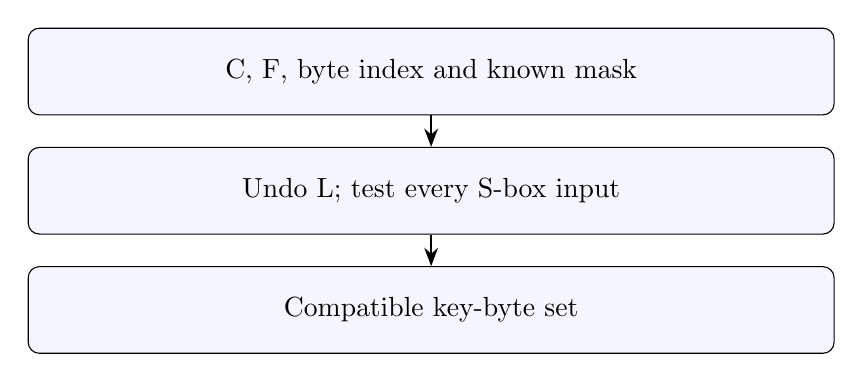
\begin{tikzpicture}[node distance=4mm]
\node[box,text width=100mm] (input) {C, F, byte index and known mask};
\node[box,below=of input,text width=100mm] (action) {Undo L; test every S-box input};
\node[box,below=of action,text width=100mm] (output) {Compatible key-byte set};
\draw[flow](input)--(action);\draw[flow](action)--(output);
\end{tikzpicture}\end{center}
\remember{\textbf{Physical interpretation:} This filtering happens on the PC after a response has been received. The known-mask assumption must be established separately for a physical experiment.}
\subsection*{Exact source}
\VerbatimInput[firstnumber=133]{generated/annotated_piret_sm4_sm4_byte_candidates.txt}
\subsection*{Read each executable line}
\begingroup\small\begin{longtable}{r >{\raggedright\arraybackslash}p{138mm}}\toprule Line&Meaning and effect\\\midrule\endfirsthead\toprule Line&Meaning and effect\\\midrule\endhead
133&Declare this callable and its parameters; the body runs only when called. Find key-byte guesses consistent with one restored ciphertext pair and a known byte fault.\\
136&Require two complete block outputs and valid controlled-fault descriptors before interpreting differences.\\
137&Stop this path with the stated exception. The message identifies the violated input, model or verification condition; no recovered key is accepted by this line.\\
139&Decode each sixteen-byte output into four big-endian unsigned 32-bit words.\\
142&Require the last three restored output words to be unchanged. Otherwise this observation violates the selected last-round model.\\
143&Stop this path with the stated exception. The message identifies the violated input, model or verification condition; no recovered key is accepted by this line.\\
146&XOR the newest words, then undo public linear diffusion to recover the S-box output difference.\\
148&Map byte 0,1,2,3 to bit shifts 24,16,8,0 in a big-endian 32-bit word.\\
150&Reject a zero difference or any nonzero difference bit outside the selected byte.\\
152&Stop this path with the stated exception. The message identifies the violated input, model or verification condition; no recovered key is accepted by this line.\\
154&Select the affected S-box output difference byte, keeping only its lowest eight bits.\\
157&Compute q: select a byte of the XOR of the three observable unchanged words. It is not a hidden state read.\\
160&Start an empty set of compatible unknown S-box input bytes.\\
162&Test each possible unknown input byte explicitly.\\
163&Apply the known error hypothesis to the candidate S-box input.\\
165&Calculate the clean/faulty S-box XOR for this candidate input and known error.\\
167&Keep the hypothesis only if its predicted S-box difference equals the observed one.\\
168&Record this compatible input value; the set removes duplicates.\\
170&Prepare key-byte candidates separately from S-box input hypotheses.\\
172&Convert each compatible S-box input into a key-byte guess.\\
173&Solve a = q XOR key\_byte using the observable q byte.\\
175&Store the resulting key-byte hypothesis for intersection with other observations.\\
177&Return the key hypotheses, compatible S-box inputs and full inverse-L difference separately.\\
\bottomrule\end{longtable}\endgroup
\section{\texttt{reverse\_sm4}}
Derive the initial key words from four consecutive recovered tail words, then remove FK.
\begin{center}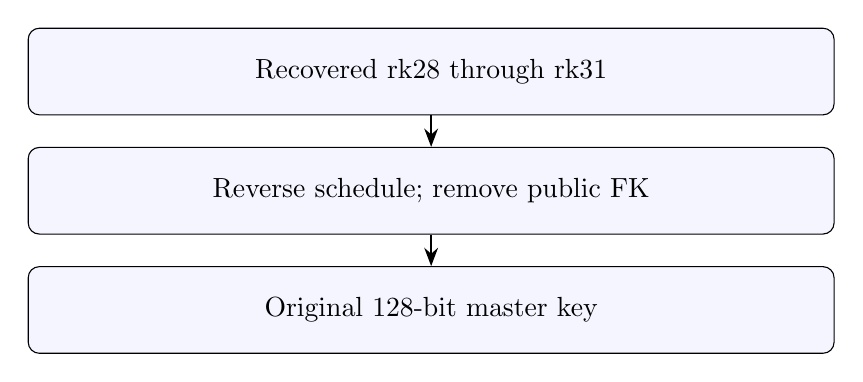
\begin{tikzpicture}[node distance=4mm]
\node[box,text width=100mm] (input) {Recovered rk28 through rk31};
\node[box,below=of input,text width=100mm] (action) {Reverse schedule; remove public FK};
\node[box,below=of action,text width=100mm] (output) {Original 128-bit master key};
\draw[flow](input)--(action);\draw[flow](action)--(output);
\end{tikzpicture}\end{center}
\remember{\textbf{Physical interpretation:} All schedule inversion runs on the PC. Public CK/FK constants are not extracted from the board.}
\subsection*{Exact source}
\VerbatimInput[firstnumber=180]{generated/annotated_piret_sm4_reverse_sm4.txt}
\subsection*{Read each executable line}
\begingroup\small\begin{longtable}{r >{\raggedright\arraybackslash}p{138mm}}\toprule Line&Meaning and effect\\\midrule\endfirsthead\toprule Line&Meaning and effect\\\midrule\endhead
180&Declare this callable and its parameters; the body runs only when called. Derive the initial key words from four consecutive recovered tail words, then remove FK.\\
183&Require four consecutive tail subkeys; a single recovered rk31 is insufficient to seed the inverse schedule.\\
184&Stop this path with the stated exception. The message identifies the violated input, model or verification condition; no recovered key is accepted by this line.\\
187&Reserve K0..K31 as unknown and seed K32..K35 with recovered rk28..rk31 in that order.\\
189&Recover schedule words in descending order so every right-hand dependency is already known.\\
192&Form the public schedule-core input from three known neighboring words and CK[index].\\
194&Apply the forward S-box and key-specific L-prime, then XOR with K[index+4] to solve for the older schedule word.\\
196&Call optional explanatory instrumentation only if supplied; the numerical result has already been computed.\\
197&Report this derived schedule word without giving the observer control over key recovery.\\
200&Prepare four unwhitened master-key words.\\
202&Remove FK separately for master-word positions zero through three.\\
203&Undo initial key whitening with the corresponding public FK constant.\\
204&Preserve the master-word order for final serialization.\\
206&Serialize the four recovered master words into sixteen big-endian bytes.\\
\bottomrule\end{longtable}\endgroup
\section{\texttt{peel\_sm4}}
Reconstruct an earlier output window using only already recovered later keys.
\begin{center}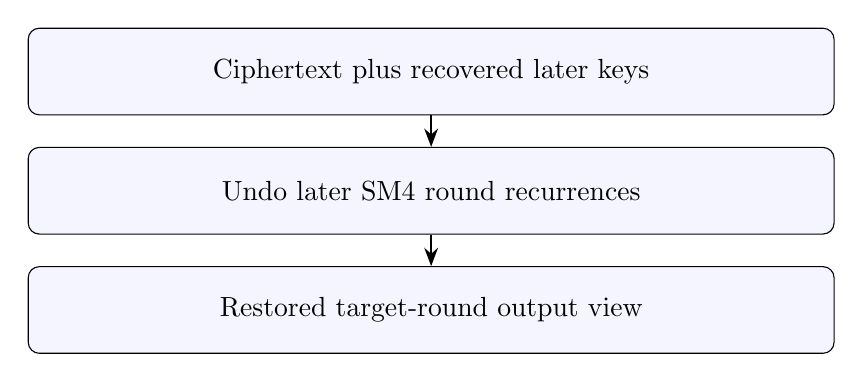
\begin{tikzpicture}[node distance=4mm]
\node[box,text width=100mm] (input) {Ciphertext plus recovered later keys};
\node[box,below=of input,text width=100mm] (action) {Undo later SM4 round recurrences};
\node[box,below=of action,text width=100mm] (output) {Restored target-round output view};
\draw[flow](input)--(action);\draw[flow](action)--(output);
\end{tikzpicture}\end{center}
\remember{\textbf{Physical interpretation:} This is offline PC computation. It neither rewinds the STM32 nor reads an old state from target RAM.}
\subsection*{Exact source}
\VerbatimInput[firstnumber=209]{generated/annotated_piret_sm4_peel_sm4.txt}
\subsection*{Read each executable line}
\begingroup\small\begin{longtable}{r >{\raggedright\arraybackslash}p{138mm}}\toprule Line&Meaning and effect\\\midrule\endfirsthead\toprule Line&Meaning and effect\\\midrule\endhead
209&Declare this callable and its parameters; the body runs only when called. Reconstruct an earlier output window using only already recovered later keys.\\
217&Reuse a sixteen-byte length check. This does not execute AES and does not import an AES key into SM4 recovery.\\
219&Restrict this full-recovery peeling helper to the four modeled target rounds.\\
220&Stop this path with the stated exception. The message identifies the violated input, model or verification condition; no recovered key is accepted by this line.\\
223&Read the four final output words, then reverse their order to restore the chronological rolling state.\\
225&Undo only rounds later than the requested target round, newest first.\\
226&Require a genuinely recovered later key before reversing its round; never substitute a reference key.\\
227&Stop this path with the stated exception. The message identifies the violated input, model or verification condition; no recovered key is accepted by this line.\\
231&Recompute the later-round nonlinear/linear transform and XOR with its newest word to reconstruct the missing oldest word.\\
233&Shift the reconstructed window backward by one round: old, u0, u1, u2.\\
236&Return a synthetic ciphertext-style view with word reversal, allowing reuse of the same last-round candidate equation.\\
\bottomrule\end{longtable}\endgroup
\section{\texttt{recover\_sm4\_master\_key}}
Coordinate independent fault observations, intersections, four tail-key recoveries and inverse key expansion.
\begin{center}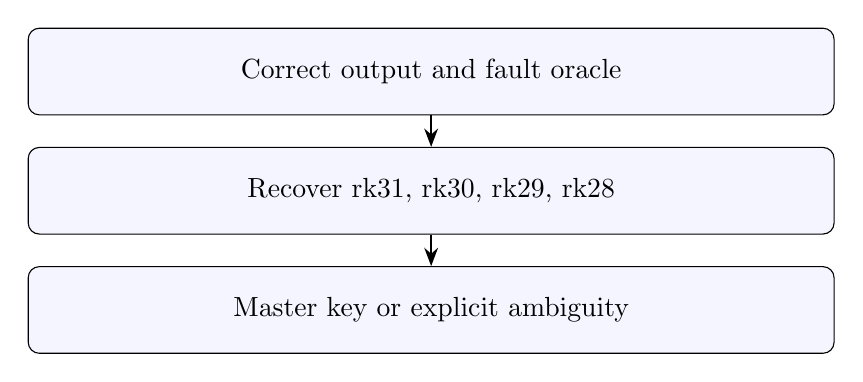
\begin{tikzpicture}[node distance=4mm]
\node[box,text width=100mm] (input) {Correct output and fault oracle};
\node[box,below=of input,text width=100mm] (action) {Recover rk31, rk30, rk29, rk28};
\node[box,below=of action,text width=100mm] (output) {Master key or explicit ambiguity};
\draw[flow](input)--(action);\draw[flow](action)--(output);
\end{tikzpicture}\end{center}
\remember{\textbf{Physical interpretation:} On hardware, each oracle request would involve another target encryption and response. The implementation here makes software calls, not USB or serial requests.}
\subsection*{Exact source}
\VerbatimInput[firstnumber=239]{generated/annotated_piret_sm4_recover_sm4_master_key.txt}
\subsection*{Read each executable line}
\begingroup\small\begin{longtable}{r >{\raggedright\arraybackslash}p{138mm}}\toprule Line&Meaning and effect\\\midrule\endfirsthead\toprule Line&Meaning and effect\\\midrule\endhead
239&Declare this callable and its parameters; the body runs only when called. Coordinate independent fault observations, intersections, four tail-key recoveries and inverse key expansion.\\
248&Reuse a sixteen-byte length check. This does not execute AES and does not import an AES key into SM4 recovery.\\
250&Freeze a possibly one-shot iterable so every target byte can reuse the same ordered observation masks.\\
252&Reject an empty fault-mask sequence before any target query.\\
253&Stop this path with the stated exception. The message identifies the violated input, model or verification condition; no recovered key is accepted by this line.\\
255&Reject repeated masks; deterministic repeated observations do not add constraints.\\
256&Stop this path with the stated exception. The message identifies the violated input, model or verification condition; no recovered key is accepted by this line.\\
258&Validate each supplied fault descriptor explicitly.\\
259&Reject zero and masks that do not fit in one nonzero byte.\\
260&Stop this path with the stated exception. The message identifies the violated input, model or verification condition; no recovered key is accepted by this line.\\
262&Require the first selected byte position to be zero through three.\\
263&Stop this path with the stated exception. The message identifies the violated input, model or verification condition; no recovered key is accepted by this line.\\
265&Initialize recovered keys, event history, per-byte counts and actual faulty-output query count separately.\\
267&Target rounds 31,30,29,28 in that order; later recovered keys enable peeling for the next target.\\
269&Restore the clean reference to this target round using only the currently recovered later keys.\\
271&Allocate four output bytes for the current round key; unfilled bytes must not be treated as recovered.\\
273&Prepare an explicit ordering of all four byte positions for this round.\\
275&Visit four offsets starting from the user-selected first byte.\\
276&Wrap the byte position modulo four so every position appears once.\\
278&Recover one complete key byte at a time in the chosen order.\\
279&Mark the byte or group as unconstrained before its first observation; an empty set would instead mean inconsistency.\\
282&Request distinct faults sequentially, numbering observations from one within this target byte/group.\\
283&Query the simulated target for one new faulty ciphertext. No key or teacher trace is returned to this solver.\\
285&Undo the same recovered later rounds in the faulty ciphertext so both outputs refer to the same target round.\\
287&Choose the default known-byte filter unless another compatible filter, such as the Giraud-inspired one, was explicitly supplied.\\
289&Apply the selected-round byte equation to this clean/faulty pair and known mask.\\
290&The if-condition at line 287 was false; follow this alternative path rather than the preceding branch.\\
291&Run the alternate filter and receive its inferred byte position alongside candidate sets and difference.\\
293&Reject an alternate-filter result whose changed byte is inconsistent with the requested target byte.\\
294&Stop this path with the stated exception. The message identifies the violated input, model or verification condition; no recovered key is accepted by this line.\\
296&Distinguish the first observation from subsequent intersections; no previous candidate set exists yet.\\
297&Before a first byte observation all 256 byte values are still possible.\\
298&The first pair initializes the byte set; subsequent pairs intersect it. No new guess can be introduced by intersection.\\
299&The if-condition at line 296 was false; follow this alternative path rather than the preceding branch.\\
300&Record the number of hypotheses remaining before applying the new observation.\\
301&Intersect the prior hypotheses with those from the new pair; never introduce a new candidate.\\
304&An empty intersection means the observations and model cannot be reconciled; do not claim a key.\\
305&Stop this path with the stated exception. The message identifies the violated input, model or verification condition; no recovered key is accepted by this line.\\
307&Count one faulty ciphertext actually consumed by the solver, not a printed stage or a schedule replay.\\
308&Store the surviving count for this particular round and byte.\\
309&Prepare a display-only dictionary of already recovered later subkeys.\\
311&Visit only subkeys already established by the solver.\\
312&Format each recovered subkey as eight hexadecimal digits for event metadata.\\
314&Package the measurement pair, restored views, known mask, input guesses, surviving key guesses and recovered peeling keys for presentation.\\
315&Preserve this observation in order for later inspection and reproducibility.\\
317&Only invoke the optional reporting callback if the caller requested it.\\
319&Pass copied event metadata to reporting. Candidate-set intersection has already been decided in the solver.\\
321&Uniqueness is the acceptance rule: one value remains compatible with all observations for this byte/group.\\
323&Extract the sole surviving byte and store it at the correct big-endian position.\\
324&Stop this observation loop immediately after uniqueness; do not query unused masks.\\
325&The for-loop beginning at line 282 exhausted its observation budget without break; execute the following ambiguity result.\\
328&Return an explicit incomplete result when the observation loop exhausts its budget without a break. No master key is selected.\\
330&Concatenate the four uniquely recovered bytes into one 32-bit round key and make it available for future peeling.\\
333&Prepare the four recovered tail keys in forward key-schedule order.\\
335&Read rk28, rk29, rk30 and rk31 in the order expected by schedule inversion.\\
336&Add the actual recovered subkey to the inverse-schedule seed.\\
338&Arrange recovered rk28..rk31 in schedule order and reverse expansion to derive the original key.\\
340&Return the complete key together with actual recovered tail keys, history, counts and fault-query cost.\\
\bottomrule\end{longtable}\endgroup
\section{\texttt{main}}
Parse the attack-specific command and enter the same SM4 terminal lesson used by run.py.
\begin{center}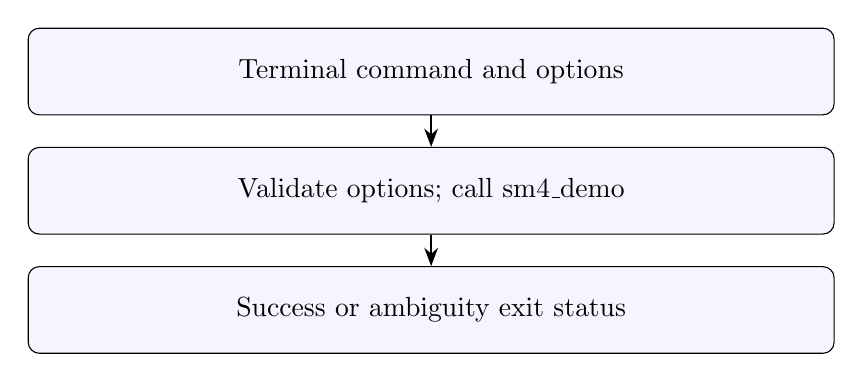
\begin{tikzpicture}[node distance=4mm]
\node[box,text width=100mm] (input) {Terminal command and options};
\node[box,below=of input,text width=100mm] (action) {Validate options; call sm4\_demo};
\node[box,below=of action,text width=100mm] (output) {Success or ambiguity exit status};
\draw[flow](input)--(action);\draw[flow](action)--(output);
\end{tikzpicture}\end{center}
\remember{\textbf{Physical interpretation:} This is a PC entry point. Selecting --row chooses a simulated byte, not a physical chip coordinate. The compatibility options --column and --seed are parsed but not used in this SM4 path.}
\subsection*{Exact source}
\VerbatimInput[firstnumber=343]{generated/annotated_piret_sm4_main.txt}
\subsection*{Read each executable line}
\begingroup\small\begin{longtable}{r >{\raggedright\arraybackslash}p{138mm}}\toprule Line&Meaning and effect\\\midrule\endfirsthead\toprule Line&Meaning and effect\\\midrule\endhead
343&Declare this callable and its parameters; the body runs only when called. Parse the attack-specific command and enter the same SM4 terminal lesson used by run.py.\\
346&Create the command-line option parser using the module description for help text.\\
348&Register --algorithm. Select the allowed cipher branch for this entry point.\\
349&Register --step. Enable pauses at teaching boundaries.\\
350&Register --color. Select automatic, forced or disabled ANSI colors.\\
351&Register --faults. Set the maximum distinct mask observations per SM4 target byte.\\
352&Register --row. Choose the first simulated SM4 byte position.\\
354&Register --column. Compatibility setting parsed but not used by this SM4 entry point.\\
355&Register --seed. Used for AES mask sampling in run.py; not used for SM4 mask order.\\
357&Decode the supplied argument list (or process command line) and enforce the declared argument types and choices.\\
359&Reject an observation budget outside 1..255 before requesting any faulty outputs.\\
360&Report invalid configuration and terminate argument processing rather than starting an invalid experiment.\\
362&Load the shared terminal controller at call time. This avoids a top-level circular import between attack and presentation modules.\\
364&Run the shared SM4 lesson and test whether full recovery verified.\\
365&Return successful process status after verified complete recovery.\\
367&Return the explicit ambiguity/failure status when full recovery was not verified.\\
\bottomrule\end{longtable}\endgroup
\chapter{Line-by-line: \texttt{run.py}}
\section{\texttt{block}}
Convert a hexadecimal input string to exactly sixteen bytes.
\begin{center}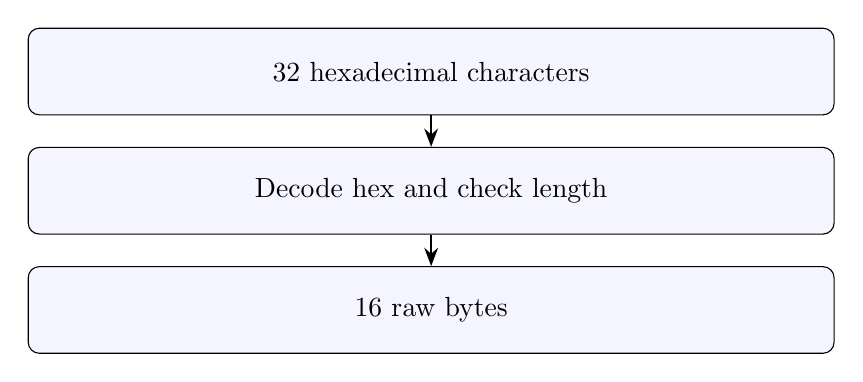
\begin{tikzpicture}[node distance=4mm]
\node[box,text width=100mm] (input) {32 hexadecimal characters};
\node[box,below=of input,text width=100mm] (action) {Decode hex and check length};
\node[box,below=of action,text width=100mm] (output) {16 raw bytes};
\draw[flow](input)--(action);\draw[flow](action)--(output);
\end{tikzpicture}\end{center}
\remember{\textbf{Physical interpretation:} A future host transport would send these bytes to firmware. This function only prepares host memory.}
\subsection*{Exact source}
\VerbatimInput[firstnumber=12]{generated/annotated_run_block.txt}
\subsection*{Read each executable line}
\begingroup\small\begin{longtable}{r >{\raggedright\arraybackslash}p{138mm}}\toprule Line&Meaning and effect\\\midrule\endfirsthead\toprule Line&Meaning and effect\\\midrule\endhead
12&Declare this callable and its parameters; the body runs only when called. Convert a hexadecimal input string to exactly sixteen bytes.\\
13&Decode hexadecimal text into raw bytes; malformed hex raises ValueError instead of silently changing the input.\\
15&Accept only one complete 128-bit block or key for this demonstration.\\
16&Stop this path with the stated exception. The message identifies the violated input, model or verification condition; no recovered key is accepted by this line.\\
18&Return the validated raw bytes used by the cipher and target simulator.\\
\bottomrule\end{longtable}\endgroup
\section{\texttt{LessonTerminal}}
Format the same data as clean/faulty/XOR rows with red differences.
\begin{center}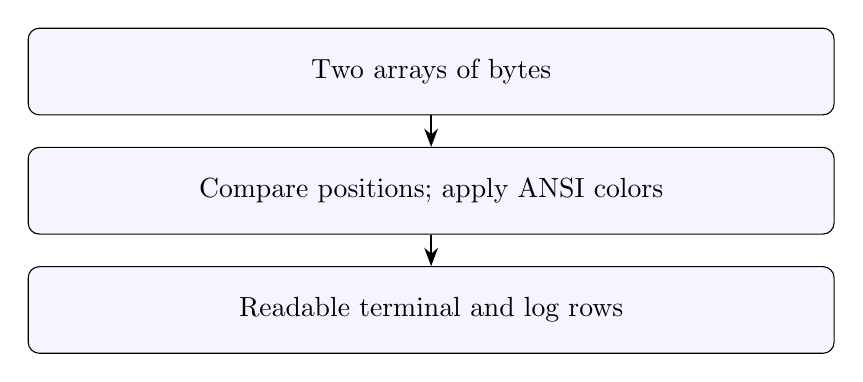
\begin{tikzpicture}[node distance=4mm]
\node[box,text width=100mm] (input) {Two arrays of bytes};
\node[box,below=of input,text width=100mm] (action) {Compare positions; apply ANSI colors};
\node[box,below=of action,text width=100mm] (output) {Readable terminal and log rows};
\draw[flow](input)--(action);\draw[flow](action)--(output);
\end{tikzpicture}\end{center}
\remember{\textbf{Physical interpretation:} Only the PC display changes. Red text is a visualization of differing data, not a measured electrical pulse.}
\subsection*{Exact source}
\VerbatimInput[firstnumber=21]{generated/annotated_run_LessonTerminal.txt}
\subsection*{Read each executable line}
\begingroup\small\begin{longtable}{r >{\raggedright\arraybackslash}p{138mm}}\toprule Line&Meaning and effect\\\midrule\endfirsthead\toprule Line&Meaning and effect\\\midrule\endhead
21&Declare this callable and its parameters; the body runs only when called. Format the same data as clean/faulty/XOR rows with red differences.\\
22&Define the byte-formatting method used to color differences without changing any byte values.\\
23&Accumulate or append the explicitly formatted hexadecimal display fragments; this does not modify cipher data.\\
25&Compare each faulty output byte with its reference position before choosing its color.\\
26&Use red formatting only when this faulty byte differs from the clean reference byte.\\
27&Prepare this changed byte with ANSI red and an immediate reset.\\
28&The if-condition at line 26 was false; follow this alternative path rather than the preceding branch.\\
29&Prepare an unchanged byte as ordinary two-digit hexadecimal text.\\
31&Accumulate or append the explicitly formatted hexadecimal display fragments; this does not modify cipher data.\\
33&Join the prepared hex fragments with spaces for terminal display.\\
35&Define the clean/faulty/XOR printing method used throughout both lessons.\\
36&Accumulate or append the explicitly formatted hexadecimal display fragments; this does not modify cipher data.\\
38&Format each clean reference byte without fault coloring.\\
39&Accumulate or append the explicitly formatted hexadecimal display fragments; this does not modify cipher data.\\
41&Print the text/label "Correct:". This is presentation output, also mirrored to the active log; it performs no target query and changes no candidates.\\
42&Print the text/label "Faulty:". This is presentation output, also mirrored to the active log; it performs no target query and changes no candidates.\\
44&Prepare an explicit byte buffer for the following comparison or recovered-key serialization.\\
46&Visit the aligned correct and faulty bytes in the same serialized order.\\
47&Append their byte XOR, which is zero exactly when the two positions agree.\\
49&Serialize the explicitly constructed difference buffer.\\
51&Print the text/label "XOR:". This is presentation output, also mirrored to the active log; it performs no target query and changes no candidates.\\
\bottomrule\end{longtable}\endgroup
\section{\texttt{aes\_demo}}
Run the AES round-9 lesson when AES is selected; this function is not executed by --algorithm sm4.
\begin{center}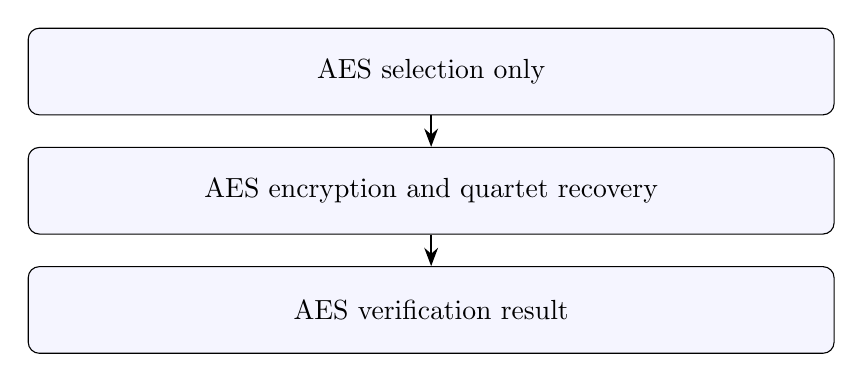
\begin{tikzpicture}[node distance=4mm]
\node[box,text width=100mm] (input) {AES selection only};
\node[box,below=of input,text width=100mm] (action) {AES encryption and quartet recovery};
\node[box,below=of action,text width=100mm] (output) {AES verification result};
\draw[flow](input)--(action);\draw[flow](action)--(output);
\end{tikzpicture}\end{center}
\remember{\textbf{Physical interpretation:} Included for complete run.py coverage. It does not contribute to SM4 recovery; all operations here remain host-side software simulation.}
\subsection*{Exact source}
\VerbatimInput[firstnumber=54]{generated/annotated_run_aes_demo.txt}
\subsection*{Read each executable line}
\begingroup\small\begin{longtable}{r >{\raggedright\arraybackslash}p{138mm}}\toprule Line&Meaning and effect\\\midrule\endfirsthead\toprule Line&Meaning and effect\\\midrule\endhead
54&Declare this callable and its parameters; the body runs only when called. Run the AES round-9 lesson when AES is selected; this function is not executed by --algorithm sm4.\\
55&Load AES simulation inputs. This line belongs to the AES branch and does not supply SM4 key material.\\
57&Print the named teaching-section boundary. This affects terminal/log organization only and does not advance the target or the solver.\\
59&Print the text/label "Plaintext:  Key:". This is presentation output, also mirrored to the active log; it performs no target query and changes no candidates.\\
60&Print the text/label "AES layout: index = 4*column + row. This execution has no fault.". This is presentation output, also mirrored to the active log; it performs no target query and changes no candidates.\\
62&Use the AES trace adapter with fault\_round=9; mask zero creates the clean reference.\\
64&Check that the trace adapter matches ordinary AES encryption before teaching its fault behavior.\\
65&Stop this path with the stated exception. The message identifies the violated input, model or verification condition; no recovered key is accepted by this line.\\
67&Compute AES round keys for the teacher-only normal-encryption display.\\
69&Show each AES expanded round key in sequence.\\
70&Print the text/label "K  =". Substitute these runtime fields: number, aes.state\_to\_bytes(round\_key).hex().upper(). This is presentation output, also mirrored to the active log; it performs no target query and changes no candidates.\\
72&Convert the plaintext into the AES column-major matrix for initial key addition.\\
74&Apply the initial AES K0 XOR in the teacher view.\\
76&Print the text/label "Initial AddRoundKey:". This is presentation output, also mirrored to the active log; it performs no target query and changes no candidates.\\
78&Walk the clean AES transformation snapshots in execution order.\\
79&Exclude the adapter marker from the ordinary AES transformation display.\\
80&Print the text/label "R   :". Substitute these runtime fields: number, operation, state.hex().upper(). This is presentation output, also mirrored to the active log; it performs no target query and changes no candidates.\\
81&Wait for Enter only if --step is enabled. Pausing does not change a state word, create a fault or alter a candidate set.\\
83&Print the text/label "Correct ciphertext:". This is presentation output, also mirrored to the active log; it performs no target query and changes no candidates.\\
85&Print the named teaching-section boundary. This affects terminal/log organization only and does not advance the target or the solver.\\
87&Print the text/label "Recover one K10 quartet per column; repeat across all four columns.". This is presentation output, also mirrored to the active log; it performs no target query and changes no candidates.\\
88&Print the text/label "d = InvSbox[C[p] XOR k] XOR InvSbox[F[p] XOR k].". This is presentation output, also mirrored to the active log; it performs no target query and changes no candidates.\\
89&Print the text/label "Four d values must match one of 4*255 = 1020 MixColumns difference patterns.". This is presentation output, also mirrored to the active log; it performs no target query and changes no candidates.\\
91&Use the two preferred initial AES masks when the observation budget allows both.\\
92&Try AES masks 1 and 2 first, then reproducibly sample other distinct nonzero masks up to the limit.\\
93&The if-condition at line 91 was false; follow this alternative path rather than the preceding branch.\\
94&For a budget of one, run only the first AES mask rather than requesting extra observations.\\
96&Prepare sixteen AES final-key bytes and a total faulty-output counter.\\
98&Recover each of the four AES pre-ShiftRows key quartets in turn.\\
99&Mark the byte or group as unconstrained before its first observation; an empty set would instead mean inconsistency.\\
101&Print the text/label "COLUMN  : output/key positions". Substitute these runtime fields: column, piret\_aes.output\_positions(column). This is presentation output, also mirrored to the active log; it performs no target query and changes no candidates.\\
103&Request distinct faults sequentially, numbering observations from one within this target byte/group.\\
104&Run an AES round-9 byte-fault encryption for the selected column and mask.\\
105&Count this faulty AES encryption once, independently of display stages.\\
106&Print the text/label "Observation  : simulator XOR  , row 0 / column  .". Substitute these runtime fields: observation, mask, column. This is presentation output, also mirrored to the active log; it performs no target query and changes no candidates.\\
107&Print the text/label "The solver enumerates unknown fault rows/values and does not receive this mask.". This is presentation output, also mirrored to the active log; it performs no target query and changes no candidates.\\
108&Index clean AES snapshots by round and operation for paired fault-propagation comparisons.\\
110&Build the clean AES snapshot lookup explicitly from each recorded round and operation.\\
111&Index the clean state by its round/operation pair for later fault-propagation comparisons.\\
113&Visit each faulty AES transformation snapshot for the current observation.\\
114&Display only the AES fault round and later propagation in this part of the lesson.\\
115&Print the text/label "R". Substitute these runtime fields: number, operation. This is presentation output, also mirrored to the active log; it performs no target query and changes no candidates.\\
116&Compare the two supplied byte arrays visually, compute their XOR and color changed positions red. The data is not modified.\\
117&Wait for Enter only if --step is enabled. Pausing does not change a state word, create a fault or alter a candidate set.\\
119&Compare the two supplied byte arrays visually, compute their XOR and color changed positions red. The data is not modified.\\
120&Print exhaustive AES byte guesses and shared-error quartet patterns; this branch is not used in SM4-only execution.\\
122&Derive compatible AES K10 quartets from correct/faulty ciphertexts, not from the printed key.\\
124&Distinguish the first observation from subsequent intersections; no previous candidate set exists yet.\\
125&Mark the initial AES quartet history as unconstrained rather than claiming a previous finite set.\\
126&The if-condition at line 124 was false; follow this alternative path rather than the preceding branch.\\
127&Record the number of hypotheses remaining before applying the new observation.\\
130&Distinguish the first observation from subsequent intersections; no previous candidate set exists yet.\\
131&Initialize this AES quartet set directly from the first observed pair.\\
132&The if-condition at line 130 was false; follow this alternative path rather than the preceding branch.\\
133&Intersect the prior hypotheses with those from the new pair; never introduce a new candidate.\\
135&Print the text/label "Candidates in this pair:  ; intersection:   ->". Substitute these runtime fields: len(fresh), before, len(survivors). This is presentation output, also mirrored to the active log; it performs no target query and changes no candidates.\\
136&Accumulate or append the explicitly formatted hexadecimal display fragments; this does not modify cipher data.\\
138&Format up to four candidates for the short summary; the earlier detailed tables remain exhaustive.\\
139&Accumulate or append the explicitly formatted hexadecimal display fragments; this does not modify cipher data.\\
141&Print the text/label "First survivors:   |". This is presentation output, also mirrored to the active log; it performs no target query and changes no candidates.\\
142&Wait for Enter only if --step is enabled. Pausing does not change a state word, create a fault or alter a candidate set.\\
144&An empty intersection means the observations and model cannot be reconciled; do not claim a key.\\
145&Stop this path with the stated exception. The message identifies the violated input, model or verification condition; no recovered key is accepted by this line.\\
147&Uniqueness is the acceptance rule: one value remains compatible with all observations for this byte/group.\\
148&Place the unique AES tuple bytes into final ciphertext/key order using inverse ShiftRows mapping.\\
149&Store one uniquely recovered AES final-key byte at its true serialized position.\\
151&Stop this observation loop immediately after uniqueness; do not query unused masks.\\
152&The for-loop beginning at line 103 exhausted its observation budget without break; execute the following ambiguity result.\\
153&Print the text/label "AES recovery remains ambiguous. Increase --observations. 31". This is presentation output, also mirrored to the active log; it performs no target query and changes no candidates.\\
154&Tell the caller that this requested lesson did not establish verified complete recovery.\\
156&Print the named teaching-section boundary. This affects terminal/log organization only and does not advance the target or the solver.\\
158&Print the text/label "Recovered K10:". This is presentation output, also mirrored to the active log; it performs no target query and changes no candidates.\\
160&Derive AES K0 from the recovered K10 through the detailed display helper.\\
162&Run and print recovered-key encryption/decryption consistency checks on the ordinary cipher.\\
164&Check the AES recovered key only after recovery: ground truth and re-encryption must both agree.\\
165&Stop this path with the stated exception. The message identifies the violated input, model or verification condition; no recovered key is accepted by this line.\\
167&Print the text/label "32 AES MASTER KEY:   / PASS (  faulty outputs)". Substitute these runtime fields: recovered.hex().upper(), total. This is presentation output, also mirrored to the active log; it performs no target query and changes no candidates.\\
169&Return verified success to the command-line controller.\\
\bottomrule\end{longtable}\endgroup
\section{\texttt{inverse\_rows}}
Delegate inverse-matrix construction to the SM4 attack module.
\begin{center}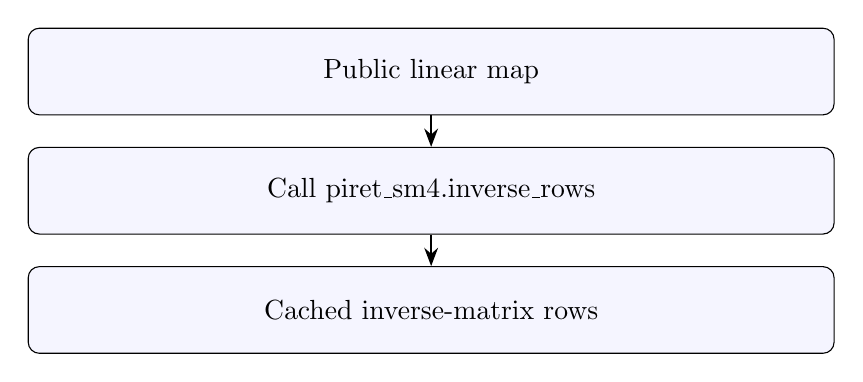
\begin{tikzpicture}[node distance=4mm]
\node[box,text width=100mm] (input) {Public linear map};
\node[box,below=of input,text width=100mm] (action) {Call piret\_sm4.inverse\_rows};
\node[box,below=of action,text width=100mm] (output) {Cached inverse-matrix rows};
\draw[flow](input)--(action);\draw[flow](action)--(output);
\end{tikzpicture}\end{center}
\remember{\textbf{Physical interpretation:} This wrapper exists on the host for compatible call sites; it does not issue a hardware operation.}
\subsection*{Exact source}
\VerbatimInput[firstnumber=172]{generated/annotated_run_inverse_rows.txt}
\subsection*{Read each executable line}
\begingroup\small\begin{longtable}{r >{\raggedright\arraybackslash}p{138mm}}\toprule Line&Meaning and effect\\\midrule\endfirsthead\toprule Line&Meaning and effect\\\midrule\endhead
172&Declare this callable and its parameters; the body runs only when called. Delegate inverse-matrix construction to the SM4 attack module.\\
175&Delegate to the single cached implementation of inverse-matrix construction.\\
\bottomrule\end{longtable}\endgroup
\section{\texttt{inverse\_linear}}
Delegate inverse diffusion to the SM4 attack module.
\begin{center}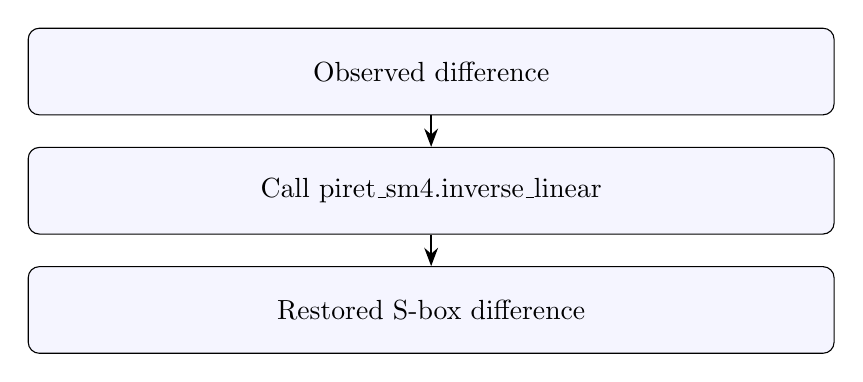
\begin{tikzpicture}[node distance=4mm]
\node[box,text width=100mm] (input) {Observed difference};
\node[box,below=of input,text width=100mm] (action) {Call piret\_sm4.inverse\_linear};
\node[box,below=of action,text width=100mm] (output) {Restored S-box difference};
\draw[flow](input)--(action);\draw[flow](action)--(output);
\end{tikzpicture}\end{center}
\remember{\textbf{Physical interpretation:} Offline PC algebra; no new target encryption occurs.}
\subsection*{Exact source}
\VerbatimInput[firstnumber=178]{generated/annotated_run_inverse_linear.txt}
\subsection*{Read each executable line}
\begingroup\small\begin{longtable}{r >{\raggedright\arraybackslash}p{138mm}}\toprule Line&Meaning and effect\\\midrule\endfirsthead\toprule Line&Meaning and effect\\\midrule\endhead
178&Declare this callable and its parameters; the body runs only when called. Delegate inverse diffusion to the SM4 attack module.\\
181&Delegate inverse diffusion; the wrapper introduces no new equation or target operation.\\
\bottomrule\end{longtable}\endgroup
\section{\texttt{sm4\_encrypt}}
Delegate a clean or faulty encryption request to the software target adapter.
\begin{center}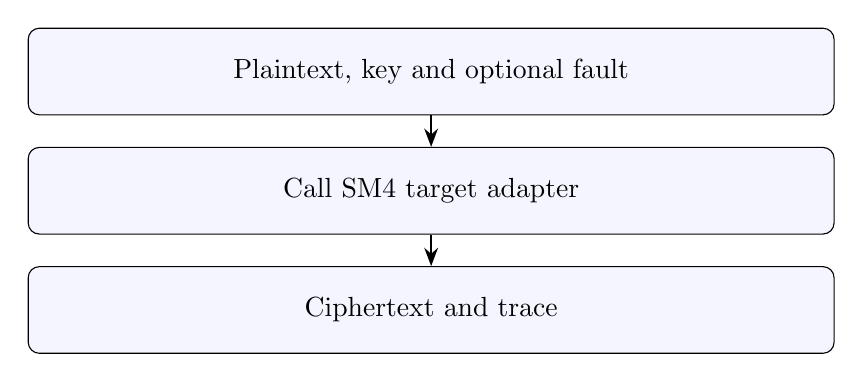
\begin{tikzpicture}[node distance=4mm]
\node[box,text width=100mm] (input) {Plaintext, key and optional fault};
\node[box,below=of input,text width=100mm] (action) {Call SM4 target adapter};
\node[box,below=of action,text width=100mm] (output) {Ciphertext and trace};
\draw[flow](input)--(action);\draw[flow](action)--(output);
\end{tikzpicture}\end{center}
\remember{\textbf{Physical interpretation:} This wrapper currently calls Python. A serial transport is not implemented by this function.}
\subsection*{Exact source}
\VerbatimInput[firstnumber=184]{generated/annotated_run_sm4_encrypt.txt}
\subsection*{Read each executable line}
\begingroup\small\begin{longtable}{r >{\raggedright\arraybackslash}p{138mm}}\toprule Line&Meaning and effect\\\midrule\endfirsthead\toprule Line&Meaning and effect\\\midrule\endhead
184&Declare this callable and its parameters; the body runs only when called. Delegate a clean or faulty encryption request to the software target adapter.\\
187&Forward the target inputs and optional fault descriptor to the SM4 simulator, returning both output and trace.\\
\bottomrule\end{longtable}\endgroup
\section{\texttt{sm4\_byte\_candidates}}
Delegate the known-mask byte equation to the attack module.
\begin{center}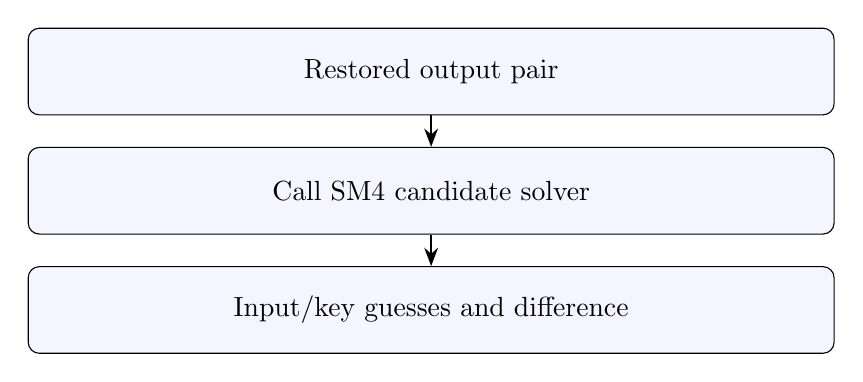
\begin{tikzpicture}[node distance=4mm]
\node[box,text width=100mm] (input) {Restored output pair};
\node[box,below=of input,text width=100mm] (action) {Call SM4 candidate solver};
\node[box,below=of action,text width=100mm] (output) {Input/key guesses and difference};
\draw[flow](input)--(action);\draw[flow](action)--(output);
\end{tikzpicture}\end{center}
\remember{\textbf{Physical interpretation:} This is PC analysis of outputs, not access to hidden chip state.}
\subsection*{Exact source}
\VerbatimInput[firstnumber=190]{generated/annotated_run_sm4_byte_candidates.txt}
\subsection*{Read each executable line}
\begingroup\small\begin{longtable}{r >{\raggedright\arraybackslash}p{138mm}}\toprule Line&Meaning and effect\\\midrule\endfirsthead\toprule Line&Meaning and effect\\\midrule\endhead
190&Declare this callable and its parameters; the body runs only when called. Delegate the known-mask byte equation to the attack module.\\
193&Delegate ciphertext-based candidate filtering rather than duplicate it in presentation code.\\
\bottomrule\end{longtable}\endgroup
\section{\texttt{reverse\_sm4}}
Delegate schedule inversion without duplicating its equations.
\begin{center}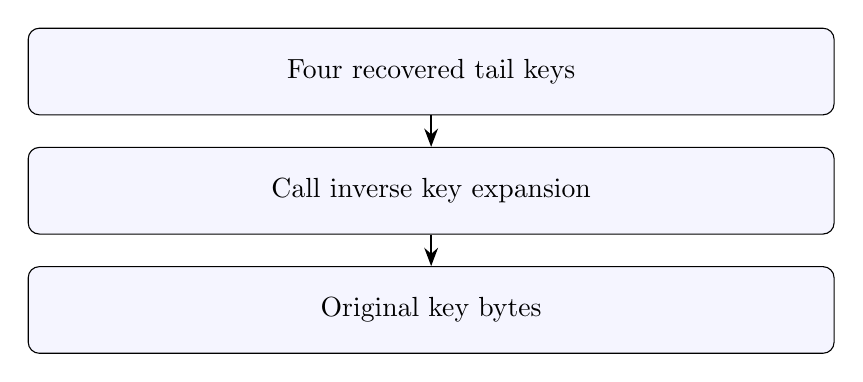
\begin{tikzpicture}[node distance=4mm]
\node[box,text width=100mm] (input) {Four recovered tail keys};
\node[box,below=of input,text width=100mm] (action) {Call inverse key expansion};
\node[box,below=of action,text width=100mm] (output) {Original key bytes};
\draw[flow](input)--(action);\draw[flow](action)--(output);
\end{tikzpicture}\end{center}
\remember{\textbf{Physical interpretation:} The host derives key material mathematically after the fault observations.}
\subsection*{Exact source}
\VerbatimInput[firstnumber=196]{generated/annotated_run_reverse_sm4.txt}
\subsection*{Read each executable line}
\begingroup\small\begin{longtable}{r >{\raggedright\arraybackslash}p{138mm}}\toprule Line&Meaning and effect\\\midrule\endfirsthead\toprule Line&Meaning and effect\\\midrule\endhead
196&Declare this callable and its parameters; the body runs only when called. Delegate schedule inversion without duplicating its equations.\\
199&Delegate schedule reversal, forwarding the optional explanatory callback.\\
\bottomrule\end{longtable}\endgroup
\section{\texttt{show\_sm4\_peeling}}
Explain every reverse round numerically for a correct or faulty output.
\begin{center}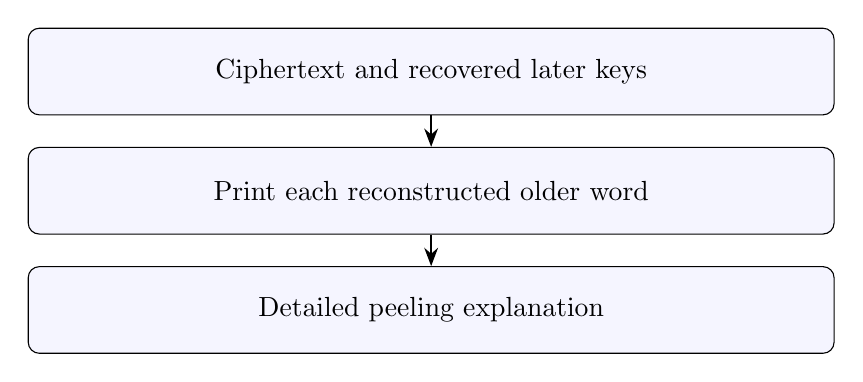
\begin{tikzpicture}[node distance=4mm]
\node[box,text width=100mm] (input) {Ciphertext and recovered later keys};
\node[box,below=of input,text width=100mm] (action) {Print each reconstructed older word};
\node[box,below=of action,text width=100mm] (output) {Detailed peeling explanation};
\draw[flow](input)--(action);\draw[flow](action)--(output);
\end{tikzpicture}\end{center}
\remember{\textbf{Physical interpretation:} This reconstructs a software view on the PC. It is not a live trace of past target registers.}
\subsection*{Exact source}
\VerbatimInput[firstnumber=202]{generated/annotated_run_show_sm4_peeling.txt}
\subsection*{Read each executable line}
\begingroup\small\begin{longtable}{r >{\raggedright\arraybackslash}p{138mm}}\toprule Line&Meaning and effect\\\midrule\endfirsthead\toprule Line&Meaning and effect\\\midrule\endhead
202&Declare this callable and its parameters; the body runs only when called. Explain every reverse round numerically for a correct or faulty output.\\
205&Start the explanatory peeling pass from the measured final ciphertext.\\
208&Undo only rounds later than the requested target round, newest first.\\
209&Restore chronological word order for the current reverse-round explanation.\\
211&Use the already recovered subkey corresponding to the later round being undone.\\
213&Form that round's S-box input from the three newest surviving words and its recovered key.\\
215&Substitute the four reconstructed input bytes using the public SM4 S-box.\\
217&Apply encryption diffusion L to the substituted value for the reverse-round equation.\\
220&Ask the actual attack helper for the restored view, so the explanatory pass cannot silently use different reversal logic.\\
222&Read the newly reconstructed oldest word from the last word of the ciphertext-style restored view.\\
224&Print the text/label "Undo round   with recovered rk =". Substitute these runtime fields: number, number, round\_key. This is presentation output, also mirrored to the active log; it performs no target query and changes no candidates.\\
225&Print the text/label "A =   XOR   XOR   XOR   =". Substitute these runtime fields: words[0], words[1], words[2], round\_key, value. This is presentation output, also mirrored to the active log; it performs no target query and changes no candidates.\\
226&Print the text/label "tau(A) =  ; L(tau(A)) =". Substitute these runtime fields: substituted, diffused. This is presentation output, also mirrored to the active log; it performs no target query and changes no candidates.\\
227&Print the text/label "X  = X  XOR L(tau(A)) =   XOR   =". Substitute these runtime fields: number, number + 4, words[3], diffused, previous. This is presentation output, also mirrored to the active log; it performs no target query and changes no candidates.\\
228&Print the text/label "Restored output view:". Substitute these runtime fields: view.hex().upper(). This is presentation output, also mirrored to the active log; it performs no target query and changes no candidates.\\
\bottomrule\end{longtable}\endgroup
\section{\texttt{show\_sm4\_key\_schedule}}
Produce and print detailed SM4 inverse-schedule teaching events.
\begin{center}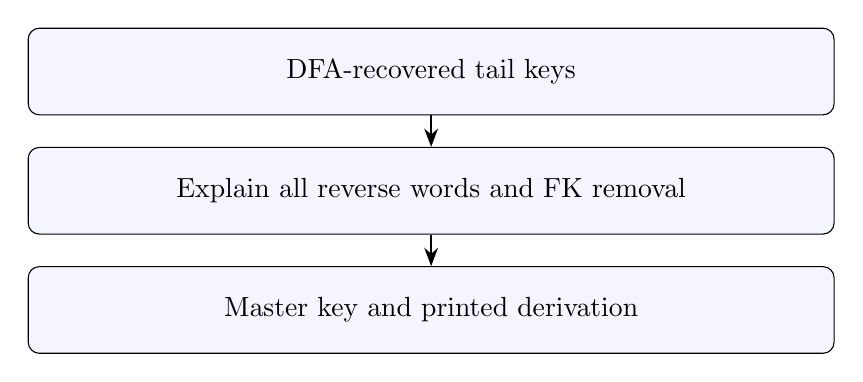
\begin{tikzpicture}[node distance=4mm]
\node[box,text width=100mm] (input) {DFA-recovered tail keys};
\node[box,below=of input,text width=100mm] (action) {Explain all reverse words and FK removal};
\node[box,below=of action,text width=100mm] (output) {Master key and printed derivation};
\draw[flow](input)--(action);\draw[flow](action)--(output);
\end{tikzpicture}\end{center}
\remember{\textbf{Physical interpretation:} This display may repeat an already completed inverse schedule. That repetition does not collect additional faults.}
\subsection*{Exact source}
\VerbatimInput[firstnumber=231]{generated/annotated_run_show_sm4_key_schedule.txt}
\subsection*{Read each executable line}
\begingroup\small\begin{longtable}{r >{\raggedright\arraybackslash}p{138mm}}\toprule Line&Meaning and effect\\\midrule\endfirsthead\toprule Line&Meaning and effect\\\midrule\endhead
231&Declare this callable and its parameters; the body runs only when called. Produce and print detailed SM4 inverse-schedule teaching events.\\
234&Build all numerical inverse-schedule events and the resulting SM4 master key from recovered tail keys.\\
236&Print the numerical teaching events already generated by the schedule helper. This is explanatory replay, not additional fault collection.\\
238&Return the master-key bytes produced by the explained inverse schedule.\\
\bottomrule\end{longtable}\endgroup
\section{\texttt{show\_sm4\_observation}}
Explain one observation, its inverse-L calculation, its candidates and its uniqueness status.
\begin{center}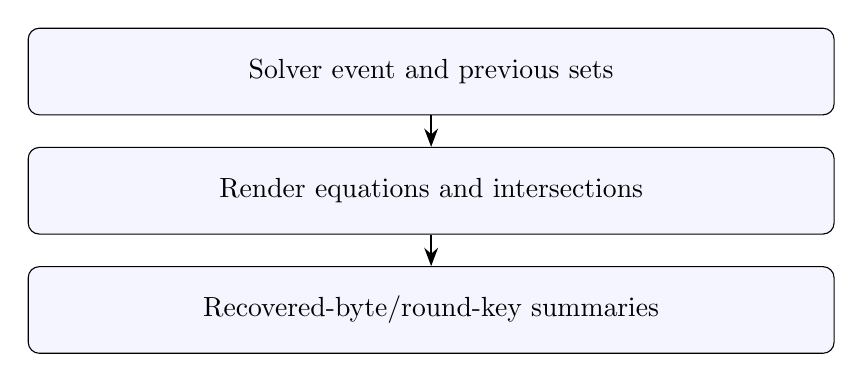
\begin{tikzpicture}[node distance=4mm]
\node[box,text width=100mm] (input) {Solver event and previous sets};
\node[box,below=of input,text width=100mm] (action) {Render equations and intersections};
\node[box,below=of action,text width=100mm] (output) {Recovered-byte/round-key summaries};
\draw[flow](input)--(action);\draw[flow](action)--(output);
\end{tikzpicture}\end{center}
\remember{\textbf{Physical interpretation:} The event contains measurements and reconstructed values. Teacher traces and hidden states must not be confused with the solver inputs.}
\subsection*{Exact source}
\VerbatimInput[firstnumber=241]{generated/annotated_run_show_sm4_observation.txt}
\subsection*{Read each executable line}
\begingroup\small\begin{longtable}{r >{\raggedright\arraybackslash}p{138mm}}\toprule Line&Meaning and effect\\\midrule\endfirsthead\toprule Line&Meaning and effect\\\midrule\endhead
241&Declare this callable and its parameters; the body runs only when called. Explain one observation, its inverse-L calculation, its candidates and its uniqueness status.\\
244&Read the selected target round and byte from the completed solver observation.\\
247&Use a compound dictionary key so candidate history for one byte cannot contaminate another round or position.\\
249&Print every detailed stage for this observation: restored views, inverse-L contributions, candidate tests and intersection. The previous display set is passed only for explanation.\\
251&Remember the current candidate set for the next detailed intersection display; this does not change the solver.\\
253&Print the round-level introduction only for the first observation of the first displayed byte.\\
254&Print the named teaching-section boundary. This affects terminal/log organization only and does not advance the target or the solver.\\
256&The actual last round requires no peeling; earlier target rounds must remove later rounds first.\\
257&Print the text/label "Round 31 is already last; no round needs to be undone.". This is presentation output, also mirrored to the active log; it performs no target query and changes no candidates.\\
258&The if-condition at line 256 was false; follow this alternative path rather than the preceding branch.\\
259&Prepare the decoded recovered-key dictionary for the explanatory peeling pass.\\
261&Decode each already recovered later key carried by the event.\\
262&Convert string indices and hexadecimal key labels back to integers for the display calculation.\\
264&Print the text/label "Restore the target round using ONLY previously recovered later subkeys.". This is presentation output, also mirrored to the active log; it performs no target query and changes no candidates.\\
265&Print the text/label "Correct execution:". This is presentation output, also mirrored to the active log; it performs no target query and changes no candidates.\\
266&Explain correct or faulty round peeling separately; these reconstructed views remain offline host values.\\
267&Print the text/label "Faulty execution (a NEW fault at the target round):". This is presentation output, also mirrored to the active log; it performs no target query and changes no candidates.\\
268&Explain correct or faulty round peeling separately; these reconstructed views remain offline host values.\\
270&Print the text/label "Round  , byte  , observation  , mask  round byte observation mask". Substitute these runtime fields: event['round'], event['byte'], event['observation'], event['mask']. This is presentation output, also mirrored to the active log; it performs no target query and changes no candidates.\\
272&Compare the two supplied byte arrays visually, compute their XOR and color changed positions red. The data is not modified.\\
274&Print the text/label "Undo later rounds using ONLY previously recovered subkeys:  peeled\_with". This is presentation output, also mirrored to the active log; it performs no target query and changes no candidates.\\
276&Compare the two supplied byte arrays visually, compute their XOR and color changed positions red. The data is not modified.\\
279&Decode the clean restored output view into four big-endian words for the explanatory equations.\\
281&Decode the corresponding faulty restored output with exactly the same layout.\\
283&Map byte 0,1,2,3 to bit shifts 24,16,8,0 in a big-endian 32-bit word.\\
285&Recompute q from public restored words for the displayed key-byte conversion.\\
287&Select the target byte of the already computed S-box output difference.\\
289&Print the text/label "DeltaX =   XOR   =". Substitute these runtime fields: clean\_words[0], faulty\_words[0], clean\_words[0] \textasciicircum{} faulty\_words[0]. This is presentation output, also mirrored to the active log; it performs no target query and changes no candidates.\\
290&Print the text/label "DeltaB = L-inverse(DeltaX) =  ; selected byte difference =  delta\_b". Substitute these runtime fields: event['delta\_b'], delta. This is presentation output, also mirrored to the active log; it performs no target query and changes no candidates.\\
291&Print the text/label "Known byte q = byte   of (X  XOR X  XOR X ) =". Substitute these runtime fields: byte, number + 1, number + 2, number + 3, known. This is presentation output, also mirrored to the active log; it performs no target query and changes no candidates.\\
294&Unknown-bit Giraud must test every one-bit mask. The default controlled-byte demonstration instead knows its mask.\\
295&List the eight possible single-bit errors without revealing which simulator bit was actually selected.\\
297&Print the text/label "UNKNOWN-BIT FILTER: the simulator mask above is NOT given to the candidate solver.". This is presentation output, also mirrored to the active log; it performs no target query and changes no candidates.\\
298&The if-condition at line 294 was false; follow this alternative path rather than the preceding branch.\\
299&Use the exact known error for the controlled-byte or explicitly known-bit model.\\
301&Print the text/label "KNOWN-MASK FILTER: the exact error is given to the candidate solver.". This is presentation output, also mirrored to the active log; it performs no target query and changes no candidates.\\
303&Accumulate or append the explicitly formatted hexadecimal display fragments; this does not modify cipher data.\\
305&Visit each value of the displayed allowed-error, survivor or recovered-byte sequence explicitly.\\
306&Accumulate or append the explicitly formatted hexadecimal display fragments; this does not modify cipher data.\\
308&Print the text/label "Allowed input errors:". This is presentation output, also mirrored to the active log; it performs no target query and changes no candidates.\\
309&Print the text/label "Test a=00..FF: at least one allowed e must satisfy S(a) XOR S(a XOR e) =  .". Substitute these runtime fields: delta. This is presentation output, also mirrored to the active log; it performs no target query and changes no candidates.\\
311&Explain every compatible S-box input that survived the current pair equation.\\
312&Start without a compatible error witness; the explicit search must find one.\\
314&Test each error permitted by the selected known-mask or unknown-bit model.\\
315&Construct the corresponding faulty S-box input for this candidate and error.\\
316&Calculate the predicted S-box difference for this error witness.\\
318&Accept the error witness only if it matches the observed byte difference.\\
319&Remember this compatible error before stopping the witness search.\\
320&Stop the permitted-error search once one compatible witness is found.\\
322&Report the impossible-witness condition rather than inventing an error value.\\
323&Stop this path with the stated exception. The message identifies the violated input, model or verification condition; no recovered key is accepted by this line.\\
325&Reconstruct the corresponding faulty S-box input for this compatible hypothesis.\\
327&Print the text/label "a= , compatible e= : S[ ] XOR S[ ] =   XOR   =  ; rk byte = a XOR q =   XOR   =". Substitute these runtime fields: candidate, error, candidate, changed, sm4.SBOX[candidate], sm4.SBOX[changed], delta, candidate, known, candidate \textasciicircum{} known. This is presentation output, also mirrored to the active log; it performs no target query and changes no candidates.\\
329&Print the text/label "L-inverse difference:  ; candidates   ->  delta\_b before remaining". Substitute these runtime fields: event['delta\_b'], event['before'], event['remaining']. This is presentation output, also mirrored to the active log; it performs no target query and changes no candidates.\\
331&Accumulate or append the explicitly formatted hexadecimal display fragments; this does not modify cipher data.\\
333&Visit each value of the displayed allowed-error, survivor or recovered-byte sequence explicitly.\\
334&Accumulate or append the explicitly formatted hexadecimal display fragments; this does not modify cipher data.\\
336&Print the text/label "Survivors:". This is presentation output, also mirrored to the active log; it performs no target query and changes no candidates.\\
338&Only print a recovered-byte declaration when the accumulated intersection has exactly one value.\\
339&Read that unique key-byte value from the sorted event list.\\
342&Maintain a per-round collection of uniquely recovered bytes for final round-key assembly.\\
344&Print the text/label "32 RECOVERED rk  byte   =   / UNIQUE". Substitute these runtime fields: number, byte, value. This is presentation output, also mirrored to the active log; it performs no target query and changes no candidates.\\
346&Wait until all four byte positions are known before claiming a complete 32-bit subkey.\\
347&Prepare an explicit byte buffer for the following comparison or recovered-key serialization.\\
349&Visit the four recovered byte positions in big-endian order.\\
350&Add the uniquely recovered byte at this position to the round-key buffer.\\
352&Serialize all four recovered bytes into the assembled round-key view.\\
353&Accumulate or append the explicitly formatted hexadecimal display fragments; this does not modify cipher data.\\
355&Visit each value of the displayed allowed-error, survivor or recovered-byte sequence explicitly.\\
356&Accumulate or append the explicitly formatted hexadecimal display fragments; this does not modify cipher data.\\
358&Print the text/label "Assemble bytes in big-endian order:   ||". This is presentation output, also mirrored to the active log; it performs no target query and changes no candidates.\\
359&Print the text/label "1;32 DFA ASSEMBLED rk  =". Substitute these runtime fields: number, ordered.hex().upper(). This is presentation output, also mirrored to the active log; it performs no target query and changes no candidates.\\
361&Wait for Enter only if --step is enabled. Pausing does not change a state word, create a fault or alter a candidate set.\\
\bottomrule\end{longtable}\endgroup
\section{\texttt{show\_aes\_key\_schedule}}
Print the AES inverse schedule; this path is inactive in the SM4 demonstration.
\begin{center}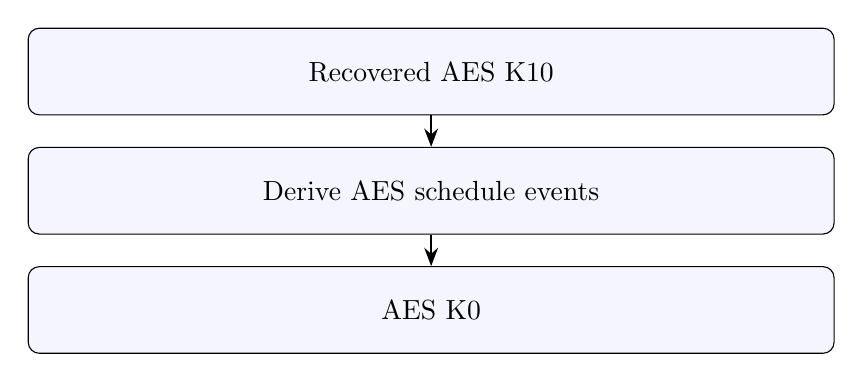
\begin{tikzpicture}[node distance=4mm]
\node[box,text width=100mm] (input) {Recovered AES K10};
\node[box,below=of input,text width=100mm] (action) {Derive AES schedule events};
\node[box,below=of action,text width=100mm] (output) {AES K0};
\draw[flow](input)--(action);\draw[flow](action)--(output);
\end{tikzpicture}\end{center}
\remember{\textbf{Physical interpretation:} Included only because it is a function in run.py. The SM4 path instead uses show\_sm4\_key\_schedule.}
\subsection*{Exact source}
\VerbatimInput[firstnumber=364]{generated/annotated_run_show_aes_key_schedule.txt}
\subsection*{Read each executable line}
\begingroup\small\begin{longtable}{r >{\raggedright\arraybackslash}p{138mm}}\toprule Line&Meaning and effect\\\midrule\endfirsthead\toprule Line&Meaning and effect\\\midrule\endhead
364&Declare this callable and its parameters; the body runs only when called. Print the AES inverse schedule; this path is inactive in the SM4 demonstration.\\
367&Build AES-specific inverse-schedule teaching events; this function is inactive for SM4-only execution.\\
369&Print the numerical teaching events already generated by the schedule helper. This is explanatory replay, not additional fault collection.\\
371&Return the master-key bytes produced by the explained inverse schedule.\\
\bottomrule\end{longtable}\endgroup
\section{\texttt{sm4\_demo}}
Build the clean reference, define target/report callbacks, recover the key and validate the result.
\begin{center}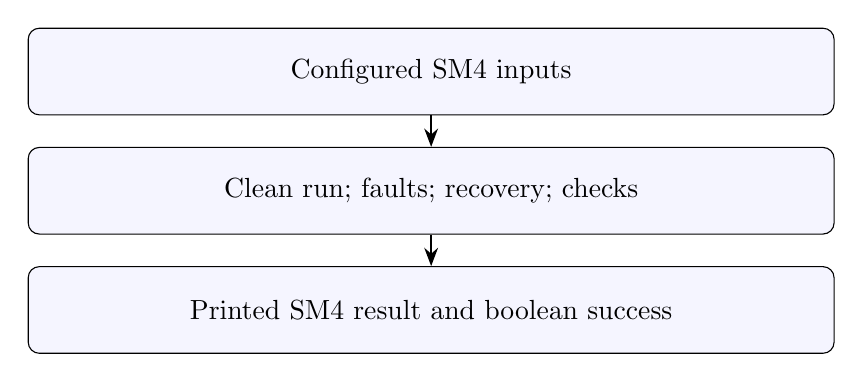
\begin{tikzpicture}[node distance=4mm]
\node[box,text width=100mm] (input) {Configured SM4 inputs};
\node[box,below=of input,text width=100mm] (action) {Clean run; faults; recovery; checks};
\node[box,below=of action,text width=100mm] (output) {Printed SM4 result and boolean success};
\draw[flow](input)--(action);\draw[flow](action)--(output);
\end{tikzpicture}\end{center}
\remember{\textbf{Physical interpretation:} This is the host experiment controller. In a board experiment the oracle would need a real transport and glitch campaign instead of the present Python target adapter.}
\subsection*{Exact source}
\VerbatimInput[firstnumber=374]{generated/annotated_run_sm4_demo.txt}
\subsection*{Read each executable line}
\begingroup\small\begin{longtable}{r >{\raggedright\arraybackslash}p{138mm}}\toprule Line&Meaning and effect\\\midrule\endfirsthead\toprule Line&Meaning and effect\\\midrule\endhead
374&Declare this callable and its parameters; the body runs only when called. Build the clean reference, define target/report callbacks, recover the key and validate the result.\\
377&Read and validate the configured target key and plaintext for simulation. The solver does not receive the key.\\
379&Run a clean reference encryption with no fault selected and retain teacher-only round records.\\
381&Print the named teaching-section boundary. This affects terminal/log organization only and does not advance the target or the solver.\\
383&Print each of the thirty-two clean encryption-round records in order.\\
384&Print the text/label "Round  : A=  B=  L(B)=  new= round a b linear new". Substitute these runtime fields: item['round'], item['a'], item['b'], item['linear'], item['new']. This is presentation output, also mirrored to the active log; it performs no target query and changes no candidates.\\
386&Wait for Enter only if --step is enabled. Pausing does not change a state word, create a fault or alter a candidate set.\\
388&Print the text/label "Ciphertext:". This is presentation output, also mirrored to the active log; it performs no target query and changes no candidates.\\
390&Print the named teaching-section boundary. This affects terminal/log organization only and does not advance the target or the solver.\\
392&Print the text/label "Controlled faults in EACH final round are required. No reference subkeys are supplied.". This is presentation output, also mirrored to the active log; it performs no target query and changes no candidates.\\
393&Print the text/label "For each byte: undo L, test S(a) XOR S(a XOR mask), then convert a to a subkey guess.". This is presentation output, also mirrored to the active log; it performs no target query and changes no candidates.\\
394&Print the text/label "Repeat independent faults and intersect guesses. Only one survivor identifies a byte.". This is presentation output, also mirrored to the active log; it performs no target query and changes no candidates.\\
396&Start presentation-only histories for candidate sets and uniquely recovered round-key bytes.\\
399&Define a target-query callback closing over the plaintext and simulated secret key. Its public result is only a ciphertext.\\
400&Perform one new target encryption with the selected fault. The detailed trace is for teaching, not solving.\\
402&Print teacher-only fault propagation from the target trace. This exposes intermediate values for learning, but none are returned as solver inputs.\\
404&Give the attacker only the target ciphertext; do not return its trace or target key.\\
406&Define the presentation callback invoked after each solver observation; it does not generate faults or choose candidates.\\
407&Render a solver event without taking control of its candidate computation.\\
409&Run full output-based SM4 recovery with mask budget 1..limit, selected starting byte and a reporting callback.\\
411&Detect an observation budget exhausted before full uniqueness; do not continue to a claimed master key.\\
412&Print the text/label "SM4 recovery remains ambiguous. Increase --observations.". This is presentation output, also mirrored to the active log; it performs no target query and changes no candidates.\\
414&Tell the caller that this requested lesson did not establish verified complete recovery.\\
416&Summarize only the four subkeys actually recovered through fault observations.\\
417&Print the text/label "32 DFA RECOVERED rk  =   / PASS". Substitute these runtime fields: number, value. This is presentation output, also mirrored to the active log; it performs no target query and changes no candidates.\\
419&Repeat inverse expansion through the detailed teaching view and retain its reconstructed master key.\\
421&Cross-check the detailed display's inverse schedule against the recovery engine's result.\\
422&Stop this path with the stated exception. The message identifies the violated input, model or verification condition; no recovered key is accepted by this line.\\
424&Run and print recovered-key encryption/decryption consistency checks on the ordinary cipher.\\
426&Re-encrypt the known plaintext with the recovered key using the ordinary SM4 cipher.\\
428&Validate both simulation ground-truth equality and the original correct ciphertext, only after recovery.\\
429&Stop this path with the stated exception. The message identifies the violated input, model or verification condition; no recovered key is accepted by this line.\\
431&Print the named teaching-section boundary. This affects terminal/log organization only and does not advance the target or the solver.\\
433&Print the text/label "Plaintext:". This is presentation output, also mirrored to the active log; it performs no target query and changes no candidates.\\
434&Print the text/label "Expected ciphertext:". This is presentation output, also mirrored to the active log; it performs no target query and changes no candidates.\\
435&Print the text/label "Recovered-key ciphertext:". This is presentation output, also mirrored to the active log; it performs no target query and changes no candidates.\\
436&Print the text/label "32  / PASS SM4 MASTER KEY:". This is presentation output, also mirrored to the active log; it performs no target query and changes no candidates.\\
437&Print the text/label "faulty outputs. All four subkeys came from DFA, not references. used". Substitute these runtime fields: result['used']. This is presentation output, also mirrored to the active log; it performs no target query and changes no candidates.\\
439&Return verified success to the command-line controller.\\
\bottomrule\end{longtable}\endgroup
\section{\texttt{main}}
Choose AES, SM4 or both and aggregate their exit status.
\begin{center}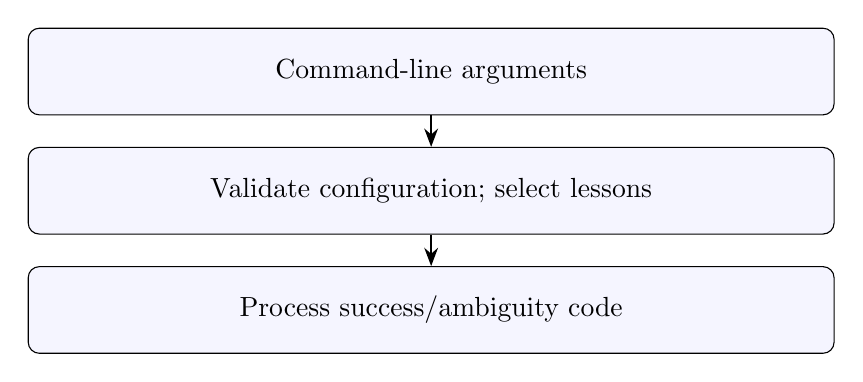
\begin{tikzpicture}[node distance=4mm]
\node[box,text width=100mm] (input) {Command-line arguments};
\node[box,below=of input,text width=100mm] (action) {Validate configuration; select lessons};
\node[box,below=of action,text width=100mm] (output) {Process success/ambiguity code};
\draw[flow](input)--(action);\draw[flow](action)--(output);
\end{tikzpicture}\end{center}
\remember{\textbf{Physical interpretation:} All selection, printing and log handling runs on the PC. --algorithm sm4 skips the AES lesson, although configuration validation checks both modules.}
\subsection*{Exact source}
\VerbatimInput[firstnumber=442]{generated/annotated_run_main.txt}
\subsection*{Read each executable line}
\begingroup\small\begin{longtable}{r >{\raggedright\arraybackslash}p{138mm}}\toprule Line&Meaning and effect\\\midrule\endfirsthead\toprule Line&Meaning and effect\\\midrule\endhead
442&Declare this callable and its parameters; the body runs only when called. Choose AES, SM4 or both and aggregate their exit status.\\
443&Create the command-line option parser using the module description for help text.\\
445&Register --algorithm. Select the allowed cipher branch for this entry point.\\
446&Register --step. Enable pauses at teaching boundaries.\\
447&Register --color. Select automatic, forced or disabled ANSI colors.\\
448&Register --observations. Set the per-byte or per-column observation budget.\\
449&Register --seed. Used for AES mask sampling in run.py; not used for SM4 mask order.\\
451&Decode the supplied argument list (or process command line) and enforce the declared argument types and choices.\\
453&Reject an observation budget outside 1..255 before requesting any faulty outputs.\\
454&Report invalid configuration and terminate argument processing rather than starting an invalid experiment.\\
456&Begin a protected configuration-validation block; the associated except path turns invalid input into a parser error.\\
457&Validate both cipher configurations even if just one lesson was requested; this is configuration checking, not AES execution.\\
458&Require this configured key or plaintext to decode as a complete block.\\
459&Catch the named validation exception and report its message through the command-line parser.\\
460&Report invalid configuration and terminate argument processing rather than starting an invalid experiment.\\
462&Configure presentation colors and optional pauses; these choices do not affect the cryptographic equations.\\
464&Print the text/label "AES\_SM4\_DFA.pdf / chapters 2-6 / software demonstration". This is presentation output, also mirrored to the active log; it performs no target query and changes no candidates.\\
465&Print the text/label "RED marks bytes changed by the injected fault, including propagated changes.". This is presentation output, also mirrored to the active log; it performs no target query and changes no candidates.\\
468&Collect independent success flags for the requested algorithm demonstrations.\\
470&Execute the AES branch only when requested. It is skipped by --algorithm sm4.\\
471&Run the AES lesson and store its success flag; not executed in the SM4-only command.\\
473&Execute the SM4 demonstration for either an explicit SM4 selection or the combined default.\\
474&Run the SM4 lesson with its observation budget and store whether full recovery verified.\\
476&Check the already collected success flags for all requested algorithm demonstrations.\\
477&Select process success because all requested demonstrations verified.\\
478&The if-condition at line 476 was false; follow this alternative path rather than the preceding branch.\\
479&Select process ambiguity status because a requested demonstration did not fully recover its key.\\
481&Return the word assembled from all thirty-two inverse-row parity calculations.\\
\bottomrule\end{longtable}\endgroup

\appendix
\chapter{All 32 clean encryption rounds}
Generated from \texttt{sm4\_fault\_encrypt()} with no fault selected. Every row corresponds to the normal terminal trace for this vector.
\begingroup\small
\begin{longtable}{rllll}
\toprule
Round & $A$ & $\tau(A)$ & $L(\tau(A))$ & New word\\
\midrule
\endfirsthead
\toprule
Round & $A$ & $\tau(A)$ & $L(\tau(A))$ & New word\\
\midrule
\endhead
0 & \texttt{F002C39E} & \texttt{18E992B1} & \texttt{26D99622} & \texttt{27FAD345}\\
1 & \texttt{EE1470AC} & \texttt{C62AD40D} & \texttt{2820815D} & \texttt{A18B4CB2}\\
2 & \texttt{AA4F1C7D} & \texttt{23A849C4} & \texttt{EF1D58B2} & \texttt{11C1E22A}\\
3 & \texttt{EC195DAA} & \texttt{C5445623} & \texttt{BA47D0FE} & \texttt{CC13E2EE}\\
4 & \texttt{4A2A2C82} & \texttt{3C0BED8A} & \texttt{DF868890} & \texttt{F87C5BD5}\\
5 & \texttt{52C45770} & \texttt{81BB8BD4} & \texttt{92A94BE5} & \texttt{33220757}\\
6 & \texttt{B1F637DF} & \texttt{DB4D95B0} & \texttt{663520BD} & \texttt{77F4C297}\\
7 & \texttt{98DCAF44} & \texttt{ADB86FF3} & \texttt{B6851005} & \texttt{7A96F2EB}\\
8 & \texttt{9B600757} & \texttt{301EB78B} & \texttt{DFA69BAA} & \texttt{27DAC07F}\\
9 & \texttt{9DE0BDBE} & \texttt{8C896C5B} & \texttt{71FF084E} & \texttt{42DD0F19}\\
10 & \texttt{DC966E60} & \texttt{B81A781E} & \texttt{CF511895} & \texttt{B8A5DA02}\\
11 & \texttt{A3474E33} & \texttt{2EBA4FA9} & \texttt{EAE7D511} & \texttt{907127FA}\\
12 & \texttt{0381926D} & \texttt{FEBF5D21} & \texttt{AC4FEBFC} & \texttt{8B952B83}\\
13 & \texttt{939943CC} & \texttt{A493FC1F} & \texttt{96F67340} & \texttt{D42B7C59}\\
14 & \texttt{8B75648F} & \texttt{CED363A1} & \texttt{97598233} & \texttt{2FFC5831}\\
15 & \texttt{60069A4A} & \texttt{1E3D323C} & \texttt{66EF4F72} & \texttt{F69E6888}\\
16 & \texttt{DC69F8C8} & \texttt{B8227911} & \texttt{24B11947} & \texttt{AF2432C4}\\
17 & \texttt{05F35DDE} & \texttt{E1EC56B4} & \texttt{3935B407} & \texttt{ED1EC85E}\\
18 & \texttt{7823DB74} & \texttt{4CF4129F} & \texttt{7A5FE213} & \texttt{55A3BA22}\\
19 & \texttt{85BD0481} & \texttt{C76CCCBF} & \texttt{E4D57022} & \texttt{124B18AA}\\
20 & \texttt{42680EC9} & \texttt{A7252CD9} & \texttt{C5C3409B} & \texttt{6AE7725F}\\
21 & \texttt{B5C5D18D} & \texttt{FDDDC161} & \texttt{19D569A7} & \texttt{F4CBA1F9}\\
22 & \texttt{4B725B6C} & \texttt{19464B01} & \texttt{486E4032} & \texttt{1DCDFA10}\\
23 & \texttt{1A00D498} & \texttt{13D6A5AD} & \texttt{3DBD1EA9} & \texttt{2FF60603}\\
24 & \texttt{716B85E6} & \texttt{003BC777} & \texttt{85153D83} & \texttt{EFF24FDC}\\
25 & \texttt{C0E8A67F} & \texttt{8D65CA9E} & \texttt{9B2FCA8C} & \texttt{6FE46B75}\\
26 & \texttt{A1C2A841} & \texttt{F6AFC007} & \texttt{94F9AABD} & \texttt{893450AD}\\
27 & \texttt{F85A7885} & \texttt{790F4CC7} & \texttt{5465894F} & \texttt{7B938F4C}\\
28 & \texttt{DFCE82C0} & \texttt{B05A8A8D} & \texttt{BC9C0D9A} & \texttt{536E4246}\\
29 & \texttt{C3E0A931} & \texttt{928929B3} & \texttt{E957823A} & \texttt{86B3E94F}\\
30 & \texttt{AF8156A0} & \texttt{6FBFDA1D} & \texttt{5B32C6F3} & \texttt{D206965E}\\
31 & \texttt{96FF9D45} & \texttt{1A488C73} & \texttt{138D5078} & \texttt{681EDF34}\\
\bottomrule
\end{longtable}
\endgroup


\chapter{All observations used in full recovery}
The fresh set uses one ciphertext pair. The intersection uses every preceding observation for the same round and byte. The displayed bytes are hexadecimal. q is computed after peeling when necessary.
\begingroup\small
\begin{longtable}{rrlllll}
\toprule
Round & Byte & $e$ & $d$ & $q$ & Fresh key guesses & Intersection\\
\midrule
\endfirsthead
\toprule
Round & Byte & $e$ & $d$ & $q$ & Fresh key guesses & Intersection\\
\midrule
\endhead
31 & 0 & \texttt{01} & \texttt{4F} & \texttt{07} & \texttt{90} \texttt{91} & \texttt{90} \texttt{91}\\
31 & 0 & \texttt{02} & \texttt{81} & \texttt{07} & \texttt{70} \texttt{72} \texttt{91} \texttt{93} & \texttt{91}\\
31 & 1 & \texttt{01} & \texttt{71} & \texttt{DB} & \texttt{24} \texttt{25} & \texttt{24} \texttt{25}\\
31 & 1 & \texttt{02} & \texttt{83} & \texttt{DB} & \texttt{24} \texttt{26} & \texttt{24}\\
31 & 2 & \texttt{01} & \texttt{79} & \texttt{3D} & \texttt{A0} \texttt{A1} & \texttt{A0} \texttt{A1}\\
31 & 2 & \texttt{02} & \texttt{6F} & \texttt{3D} & \texttt{A0} \texttt{A2} & \texttt{A0}\\
31 & 3 & \texttt{01} & \texttt{80} & \texttt{57} & \texttt{12} \texttt{13} & \texttt{12} \texttt{13}\\
31 & 3 & \texttt{02} & \texttt{C9} & \texttt{57} & \texttt{10} \texttt{12} & \texttt{12}\\
30 & 0 & \texttt{01} & \texttt{21} & \texttt{AE} & \texttt{00} \texttt{01} & \texttt{00} \texttt{01}\\
30 & 0 & \texttt{02} & \texttt{3C} & \texttt{AE} & \texttt{01} \texttt{03} & \texttt{01}\\
30 & 1 & \texttt{01} & \texttt{55} & \texttt{4E} & \texttt{CE} \texttt{CF} & \texttt{CE} \texttt{CF}\\
30 & 1 & \texttt{02} & \texttt{6D} & \texttt{4E} & \texttt{CD} \texttt{CF} & \texttt{CF}\\
30 & 2 & \texttt{01} & \texttt{51} & \texttt{24} & \texttt{72} \texttt{73} & \texttt{72} \texttt{73}\\
30 & 2 & \texttt{02} & \texttt{AB} & \texttt{24} & \texttt{70} \texttt{72} & \texttt{72}\\
30 & 3 & \texttt{01} & \texttt{EB} & \texttt{45} & \texttt{E4} \texttt{E5} & \texttt{E4} \texttt{E5}\\
30 & 3 & \texttt{02} & \texttt{FF} & \texttt{45} & \texttt{E5} \texttt{E7} & \texttt{E5}\\
29 & 0 & \texttt{01} & \texttt{3D} & \texttt{A1} & \texttt{62} \texttt{63} & \texttt{62} \texttt{63}\\
29 & 0 & \texttt{02} & \texttt{89} & \texttt{A1} & \texttt{60} \texttt{62} & \texttt{62}\\
29 & 1 & \texttt{01} & \texttt{E0} & \texttt{C9} & \texttt{28} \texttt{29} & \texttt{28} \texttt{29}\\
29 & 1 & \texttt{02} & \texttt{1E} & \texttt{C9} & \texttt{29} \texttt{2B} & \texttt{29}\\
29 & 2 & \texttt{01} & \texttt{E9} & \texttt{9D} & \texttt{34} \texttt{35} & \texttt{34} \texttt{35}\\
29 & 2 & \texttt{02} & \texttt{82} & \texttt{9D} & \texttt{34} \texttt{36} & \texttt{34}\\
29 & 3 & \texttt{01} & \texttt{57} & \texttt{A7} & \texttt{96} \texttt{97} & \texttt{96} \texttt{97}\\
29 & 3 & \texttt{02} & \texttt{1A} & \texttt{A7} & \texttt{94} \texttt{96} & \texttt{96}\\
28 & 0 & \texttt{01} & \texttt{04} & \texttt{9D} & \texttt{42} \texttt{43} & \texttt{42} \texttt{43}\\
28 & 0 & \texttt{02} & \texttt{55} & \texttt{9D} & \texttt{40} \texttt{42} & \texttt{42}\\
28 & 1 & \texttt{01} & \texttt{82} & \texttt{43} & \texttt{8C} \texttt{8D} & \texttt{8C} \texttt{8D}\\
28 & 1 & \texttt{02} & \texttt{45} & \texttt{43} & \texttt{8D} \texttt{8F} & \texttt{8D}\\
28 & 2 & \texttt{01} & \texttt{58} & \texttt{B4} & \texttt{36} \texttt{37} & \texttt{36} \texttt{37}\\
28 & 2 & \texttt{02} & \texttt{60} & \texttt{B4} & \texttt{34} \texttt{36} & \texttt{36}\\
28 & 3 & \texttt{01} & \texttt{96} & \texttt{94} & \texttt{54} \texttt{55} & \texttt{54} \texttt{55}\\
28 & 3 & \texttt{02} & \texttt{22} & \texttt{94} & \texttt{54} \texttt{56} & \texttt{54}\\
\bottomrule
\end{longtable}
\endgroup


\chapter{All inverse-L bit contributions for the first fault}
Input \(\Delta X=\hx{734E3D3D}\). Bit 0 is the least significant bit. The final running XOR is \(\Delta B=\hx{4F000000}\).
\begingroup\small
\begin{longtable}{rrlll}
\toprule
Bit & Input & Inverse basis & Contribution & Running XOR\\
\midrule
\endfirsthead
\toprule
Bit & Input & Inverse basis & Contribution & Running XOR\\
\midrule
\endhead
0 & 1 & \texttt{41455115} & \texttt{41455115} & \texttt{41455115}\\
1 & 0 & \texttt{828AA22A} & \texttt{00000000} & \texttt{41455115}\\
2 & 1 & \texttt{05154455} & \texttt{05154455} & \texttt{44501540}\\
3 & 1 & \texttt{0A2A88AA} & \texttt{0A2A88AA} & \texttt{4E7A9DEA}\\
4 & 1 & \texttt{14551154} & \texttt{14551154} & \texttt{5A2F8CBE}\\
5 & 1 & \texttt{28AA22A8} & \texttt{28AA22A8} & \texttt{7285AE16}\\
6 & 0 & \texttt{51544550} & \texttt{00000000} & \texttt{7285AE16}\\
7 & 0 & \texttt{A2A88AA0} & \texttt{00000000} & \texttt{7285AE16}\\
8 & 1 & \texttt{45511541} & \texttt{45511541} & \texttt{37D4BB57}\\
9 & 0 & \texttt{8AA22A82} & \texttt{00000000} & \texttt{37D4BB57}\\
10 & 1 & \texttt{15445505} & \texttt{15445505} & \texttt{2290EE52}\\
11 & 1 & \texttt{2A88AA0A} & \texttt{2A88AA0A} & \texttt{08184458}\\
12 & 1 & \texttt{55115414} & \texttt{55115414} & \texttt{5D09104C}\\
13 & 1 & \texttt{AA22A828} & \texttt{AA22A828} & \texttt{F72BB864}\\
14 & 0 & \texttt{54455051} & \texttt{00000000} & \texttt{F72BB864}\\
15 & 0 & \texttt{A88AA0A2} & \texttt{00000000} & \texttt{F72BB864}\\
16 & 0 & \texttt{51154145} & \texttt{00000000} & \texttt{F72BB864}\\
17 & 1 & \texttt{A22A828A} & \texttt{A22A828A} & \texttt{55013AEE}\\
18 & 1 & \texttt{44550515} & \texttt{44550515} & \texttt{11543FFB}\\
19 & 1 & \texttt{88AA0A2A} & \texttt{88AA0A2A} & \texttt{99FE35D1}\\
20 & 0 & \texttt{11541455} & \texttt{00000000} & \texttt{99FE35D1}\\
21 & 0 & \texttt{22A828AA} & \texttt{00000000} & \texttt{99FE35D1}\\
22 & 1 & \texttt{45505154} & \texttt{45505154} & \texttt{DCAE6485}\\
23 & 0 & \texttt{8AA0A2A8} & \texttt{00000000} & \texttt{DCAE6485}\\
24 & 1 & \texttt{15414551} & \texttt{15414551} & \texttt{C9EF21D4}\\
25 & 1 & \texttt{2A828AA2} & \texttt{2A828AA2} & \texttt{E36DAB76}\\
26 & 0 & \texttt{55051544} & \texttt{00000000} & \texttt{E36DAB76}\\
27 & 0 & \texttt{AA0A2A88} & \texttt{00000000} & \texttt{E36DAB76}\\
28 & 1 & \texttt{54145511} & \texttt{54145511} & \texttt{B779FE67}\\
29 & 1 & \texttt{A828AA22} & \texttt{A828AA22} & \texttt{1F515445}\\
30 & 1 & \texttt{50515445} & \texttt{50515445} & \texttt{4F000000}\\
31 & 0 & \texttt{A0A2A88A} & \texttt{00000000} & \texttt{4F000000}\\
\bottomrule
\end{longtable}
\endgroup


\chapter{All 256 candidate inputs for the first two faults}
Both observations concern rk31 byte 0. The known byte is \(q=07\). Column \(a\xor07\) converts an input guess to a key guess. Only inputs marked ACCEPT contribute to that observation's fresh set. The solver intersects the resulting \emph{key} sets.
\begingroup\small
\begin{longtable}{lllllll}
\toprule
$a$ & $S(a)$ & $d$ for $e=01$ & $d=4F$? & $d$ for $e=02$ & $d=81$? & $a\oplus07$\\
\midrule
\endfirsthead
\toprule
$a$ & $S(a)$ & $d$ for $e=01$ & $d=4F$? & $d$ for $e=02$ & $d=81$? & $a\oplus07$\\
\midrule
\endhead
\texttt{00} & \texttt{D6} & \texttt{46} & reject & \texttt{3F} & reject & \texttt{07}\\
\texttt{01} & \texttt{90} & \texttt{46} & reject & \texttt{6E} & reject & \texttt{06}\\
\texttt{02} & \texttt{E9} & \texttt{17} & reject & \texttt{3F} & reject & \texttt{05}\\
\texttt{03} & \texttt{FE} & \texttt{17} & reject & \texttt{6E} & reject & \texttt{04}\\
\texttt{04} & \texttt{CC} & \texttt{2D} & reject & \texttt{F1} & reject & \texttt{03}\\
\texttt{05} & \texttt{E1} & \texttt{2D} & reject & \texttt{56} & reject & \texttt{02}\\
\texttt{06} & \texttt{3D} & \texttt{8A} & reject & \texttt{F1} & reject & \texttt{01}\\
\texttt{07} & \texttt{B7} & \texttt{8A} & reject & \texttt{56} & reject & \texttt{00}\\
\texttt{08} & \texttt{16} & \texttt{A0} & reject & \texttt{02} & reject & \texttt{0F}\\
\texttt{09} & \texttt{B6} & \texttt{A0} & reject & \texttt{74} & reject & \texttt{0E}\\
\texttt{0A} & \texttt{14} & \texttt{D6} & reject & \texttt{02} & reject & \texttt{0D}\\
\texttt{0B} & \texttt{C2} & \texttt{D6} & reject & \texttt{74} & reject & \texttt{0C}\\
\texttt{0C} & \texttt{28} & \texttt{D3} & reject & \texttt{04} & reject & \texttt{0B}\\
\texttt{0D} & \texttt{FB} & \texttt{D3} & reject & \texttt{FE} & reject & \texttt{0A}\\
\texttt{0E} & \texttt{2C} & \texttt{29} & reject & \texttt{04} & reject & \texttt{09}\\
\texttt{0F} & \texttt{05} & \texttt{29} & reject & \texttt{FE} & reject & \texttt{08}\\
\texttt{10} & \texttt{2B} & \texttt{4C} & reject & \texttt{B1} & reject & \texttt{17}\\
\texttt{11} & \texttt{67} & \texttt{4C} & reject & \texttt{11} & reject & \texttt{16}\\
\texttt{12} & \texttt{9A} & \texttt{EC} & reject & \texttt{B1} & reject & \texttt{15}\\
\texttt{13} & \texttt{76} & \texttt{EC} & reject & \texttt{11} & reject & \texttt{14}\\
\texttt{14} & \texttt{2A} & \texttt{94} & reject & \texttt{2E} & reject & \texttt{13}\\
\texttt{15} & \texttt{BE} & \texttt{94} & reject & \texttt{7D} & reject & \texttt{12}\\
\texttt{16} & \texttt{04} & \texttt{C7} & reject & \texttt{2E} & reject & \texttt{11}\\
\texttt{17} & \texttt{C3} & \texttt{C7} & reject & \texttt{7D} & reject & \texttt{10}\\
\texttt{18} & \texttt{AA} & \texttt{EE} & reject & \texttt{B9} & reject & \texttt{1F}\\
\texttt{19} & \texttt{44} & \texttt{EE} & reject & \texttt{62} & reject & \texttt{1E}\\
\texttt{1A} & \texttt{13} & \texttt{35} & reject & \texttt{B9} & reject & \texttt{1D}\\
\texttt{1B} & \texttt{26} & \texttt{35} & reject & \texttt{62} & reject & \texttt{1C}\\
\texttt{1C} & \texttt{49} & \texttt{CF} & reject & \texttt{4F} & reject & \texttt{1B}\\
\texttt{1D} & \texttt{86} & \texttt{CF} & reject & \texttt{1F} & reject & \texttt{1A}\\
\texttt{1E} & \texttt{06} & \texttt{9F} & reject & \texttt{4F} & reject & \texttt{19}\\
\texttt{1F} & \texttt{99} & \texttt{9F} & reject & \texttt{1F} & reject & \texttt{18}\\
\texttt{20} & \texttt{9C} & \texttt{DE} & reject & \texttt{CC} & reject & \texttt{27}\\
\texttt{21} & \texttt{42} & \texttt{DE} & reject & \texttt{B6} & reject & \texttt{26}\\
\texttt{22} & \texttt{50} & \texttt{A4} & reject & \texttt{CC} & reject & \texttt{25}\\
\texttt{23} & \texttt{F4} & \texttt{A4} & reject & \texttt{B6} & reject & \texttt{24}\\
\texttt{24} & \texttt{91} & \texttt{7E} & reject & \texttt{09} & reject & \texttt{23}\\
\texttt{25} & \texttt{EF} & \texttt{7E} & reject & \texttt{95} & reject & \texttt{22}\\
\texttt{26} & \texttt{98} & \texttt{E2} & reject & \texttt{09} & reject & \texttt{21}\\
\texttt{27} & \texttt{7A} & \texttt{E2} & reject & \texttt{95} & reject & \texttt{20}\\
\texttt{28} & \texttt{33} & \texttt{67} & reject & \texttt{38} & reject & \texttt{2F}\\
\texttt{29} & \texttt{54} & \texttt{67} & reject & \texttt{17} & reject & \texttt{2E}\\
\texttt{2A} & \texttt{0B} & \texttt{48} & reject & \texttt{38} & reject & \texttt{2D}\\
\texttt{2B} & \texttt{43} & \texttt{48} & reject & \texttt{17} & reject & \texttt{2C}\\
\texttt{2C} & \texttt{ED} & \texttt{22} & reject & \texttt{41} & reject & \texttt{2B}\\
\texttt{2D} & \texttt{CF} & \texttt{22} & reject & \texttt{AD} & reject & \texttt{2A}\\
\texttt{2E} & \texttt{AC} & \texttt{CE} & reject & \texttt{41} & reject & \texttt{29}\\
\texttt{2F} & \texttt{62} & \texttt{CE} & reject & \texttt{AD} & reject & \texttt{28}\\
\texttt{30} & \texttt{E4} & \texttt{57} & reject & \texttt{F8} & reject & \texttt{37}\\
\texttt{31} & \texttt{B3} & \texttt{57} & reject & \texttt{1A} & reject & \texttt{36}\\
\texttt{32} & \texttt{1C} & \texttt{B5} & reject & \texttt{F8} & reject & \texttt{35}\\
\texttt{33} & \texttt{A9} & \texttt{B5} & reject & \texttt{1A} & reject & \texttt{34}\\
\texttt{34} & \texttt{C9} & \texttt{C1} & reject & \texttt{21} & reject & \texttt{33}\\
\texttt{35} & \texttt{08} & \texttt{C1} & reject & \texttt{9D} & reject & \texttt{32}\\
\texttt{36} & \texttt{E8} & \texttt{7D} & reject & \texttt{21} & reject & \texttt{31}\\
\texttt{37} & \texttt{95} & \texttt{7D} & reject & \texttt{9D} & reject & \texttt{30}\\
\texttt{38} & \texttt{80} & \texttt{5F} & reject & \texttt{14} & reject & \texttt{3F}\\
\texttt{39} & \texttt{DF} & \texttt{5F} & reject & \texttt{25} & reject & \texttt{3E}\\
\texttt{3A} & \texttt{94} & \texttt{6E} & reject & \texttt{14} & reject & \texttt{3D}\\
\texttt{3B} & \texttt{FA} & \texttt{6E} & reject & \texttt{25} & reject & \texttt{3C}\\
\texttt{3C} & \texttt{75} & \texttt{FA} & reject & \texttt{4A} & reject & \texttt{3B}\\
\texttt{3D} & \texttt{8F} & \texttt{FA} & reject & \texttt{29} & reject & \texttt{3A}\\
\texttt{3E} & \texttt{3F} & \texttt{99} & reject & \texttt{4A} & reject & \texttt{39}\\
\texttt{3F} & \texttt{A6} & \texttt{99} & reject & \texttt{29} & reject & \texttt{38}\\
\texttt{40} & \texttt{47} & \texttt{40} & reject & \texttt{E0} & reject & \texttt{47}\\
\texttt{41} & \texttt{07} & \texttt{40} & reject & \texttt{FB} & reject & \texttt{46}\\
\texttt{42} & \texttt{A7} & \texttt{5B} & reject & \texttt{E0} & reject & \texttt{45}\\
\texttt{43} & \texttt{FC} & \texttt{5B} & reject & \texttt{FB} & reject & \texttt{44}\\
\texttt{44} & \texttt{F3} & \texttt{80} & reject & \texttt{E4} & reject & \texttt{43}\\
\texttt{45} & \texttt{73} & \texttt{80} & reject & \texttt{C9} & reject & \texttt{42}\\
\texttt{46} & \texttt{17} & \texttt{AD} & reject & \texttt{E4} & reject & \texttt{41}\\
\texttt{47} & \texttt{BA} & \texttt{AD} & reject & \texttt{C9} & reject & \texttt{40}\\
\texttt{48} & \texttt{83} & \texttt{DA} & reject & \texttt{BF} & reject & \texttt{4F}\\
\texttt{49} & \texttt{59} & \texttt{DA} & reject & \texttt{40} & reject & \texttt{4E}\\
\texttt{4A} & \texttt{3C} & \texttt{25} & reject & \texttt{BF} & reject & \texttt{4D}\\
\texttt{4B} & \texttt{19} & \texttt{25} & reject & \texttt{40} & reject & \texttt{4C}\\
\texttt{4C} & \texttt{E6} & \texttt{63} & reject & \texttt{A9} & reject & \texttt{4B}\\
\texttt{4D} & \texttt{85} & \texttt{63} & reject & \texttt{2D} & reject & \texttt{4A}\\
\texttt{4E} & \texttt{4F} & \texttt{E7} & reject & \texttt{A9} & reject & \texttt{49}\\
\texttt{4F} & \texttt{A8} & \texttt{E7} & reject & \texttt{2D} & reject & \texttt{48}\\
\texttt{50} & \texttt{68} & \texttt{03} & reject & \texttt{E9} & reject & \texttt{57}\\
\texttt{51} & \texttt{6B} & \texttt{03} & reject & \texttt{D9} & reject & \texttt{56}\\
\texttt{52} & \texttt{81} & \texttt{33} & reject & \texttt{E9} & reject & \texttt{55}\\
\texttt{53} & \texttt{B2} & \texttt{33} & reject & \texttt{D9} & reject & \texttt{54}\\
\texttt{54} & \texttt{71} & \texttt{15} & reject & \texttt{AB} & reject & \texttt{53}\\
\texttt{55} & \texttt{64} & \texttt{15} & reject & \texttt{EF} & reject & \texttt{52}\\
\texttt{56} & \texttt{DA} & \texttt{51} & reject & \texttt{AB} & reject & \texttt{51}\\
\texttt{57} & \texttt{8B} & \texttt{51} & reject & \texttt{EF} & reject & \texttt{50}\\
\texttt{58} & \texttt{F8} & \texttt{13} & reject & \texttt{F7} & reject & \texttt{5F}\\
\texttt{59} & \texttt{EB} & \texttt{13} & reject & \texttt{A0} & reject & \texttt{5E}\\
\texttt{5A} & \texttt{0F} & \texttt{44} & reject & \texttt{F7} & reject & \texttt{5D}\\
\texttt{5B} & \texttt{4B} & \texttt{44} & reject & \texttt{A0} & reject & \texttt{5C}\\
\texttt{5C} & \texttt{70} & \texttt{26} & reject & \texttt{ED} & reject & \texttt{5B}\\
\texttt{5D} & \texttt{56} & \texttt{26} & reject & \texttt{63} & reject & \texttt{5A}\\
\texttt{5E} & \texttt{9D} & \texttt{A8} & reject & \texttt{ED} & reject & \texttt{59}\\
\texttt{5F} & \texttt{35} & \texttt{A8} & reject & \texttt{63} & reject & \texttt{58}\\
\texttt{60} & \texttt{1E} & \texttt{3A} & reject & \texttt{10} & reject & \texttt{67}\\
\texttt{61} & \texttt{24} & \texttt{3A} & reject & \texttt{7A} & reject & \texttt{66}\\
\texttt{62} & \texttt{0E} & \texttt{50} & reject & \texttt{10} & reject & \texttt{65}\\
\texttt{63} & \texttt{5E} & \texttt{50} & reject & \texttt{7A} & reject & \texttt{64}\\
\texttt{64} & \texttt{63} & \texttt{3B} & reject & \texttt{B2} & reject & \texttt{63}\\
\texttt{65} & \texttt{58} & \texttt{3B} & reject & \texttt{FA} & reject & \texttt{62}\\
\texttt{66} & \texttt{D1} & \texttt{73} & reject & \texttt{B2} & reject & \texttt{61}\\
\texttt{67} & \texttt{A2} & \texttt{73} & reject & \texttt{FA} & reject & \texttt{60}\\
\texttt{68} & \texttt{25} & \texttt{07} & reject & \texttt{59} & reject & \texttt{6F}\\
\texttt{69} & \texttt{22} & \texttt{07} & reject & \texttt{19} & reject & \texttt{6E}\\
\texttt{6A} & \texttt{7C} & \texttt{47} & reject & \texttt{59} & reject & \texttt{6D}\\
\texttt{6B} & \texttt{3B} & \texttt{47} & reject & \texttt{19} & reject & \texttt{6C}\\
\texttt{6C} & \texttt{01} & \texttt{20} & reject & \texttt{79} & reject & \texttt{6B}\\
\texttt{6D} & \texttt{21} & \texttt{20} & reject & \texttt{A6} & reject & \texttt{6A}\\
\texttt{6E} & \texttt{78} & \texttt{FF} & reject & \texttt{79} & reject & \texttt{69}\\
\texttt{6F} & \texttt{87} & \texttt{FF} & reject & \texttt{A6} & reject & \texttt{68}\\
\texttt{70} & \texttt{D4} & \texttt{D4} & reject & \texttt{92} & reject & \texttt{77}\\
\texttt{71} & \texttt{00} & \texttt{D4} & reject & \texttt{57} & reject & \texttt{76}\\
\texttt{72} & \texttt{46} & \texttt{11} & reject & \texttt{92} & reject & \texttt{75}\\
\texttt{73} & \texttt{57} & \texttt{11} & reject & \texttt{57} & reject & \texttt{74}\\
\texttt{74} & \texttt{9F} & \texttt{4C} & reject & \texttt{B8} & reject & \texttt{73}\\
\texttt{75} & \texttt{D3} & \texttt{4C} & reject & \texttt{81} & ACCEPT & \texttt{72}\\
\texttt{76} & \texttt{27} & \texttt{75} & reject & \texttt{B8} & reject & \texttt{71}\\
\texttt{77} & \texttt{52} & \texttt{75} & reject & \texttt{81} & ACCEPT & \texttt{70}\\
\texttt{78} & \texttt{4C} & \texttt{7A} & reject & \texttt{4E} & reject & \texttt{7F}\\
\texttt{79} & \texttt{36} & \texttt{7A} & reject & \texttt{D1} & reject & \texttt{7E}\\
\texttt{7A} & \texttt{02} & \texttt{E5} & reject & \texttt{4E} & reject & \texttt{7D}\\
\texttt{7B} & \texttt{E7} & \texttt{E5} & reject & \texttt{D1} & reject & \texttt{7C}\\
\texttt{7C} & \texttt{A0} & \texttt{64} & reject & \texttt{68} & reject & \texttt{7B}\\
\texttt{7D} & \texttt{C4} & \texttt{64} & reject & \texttt{5A} & reject & \texttt{7A}\\
\texttt{7E} & \texttt{C8} & \texttt{56} & reject & \texttt{68} & reject & \texttt{79}\\
\texttt{7F} & \texttt{9E} & \texttt{56} & reject & \texttt{5A} & reject & \texttt{78}\\
\texttt{80} & \texttt{EA} & \texttt{55} & reject & \texttt{60} & reject & \texttt{87}\\
\texttt{81} & \texttt{BF} & \texttt{55} & reject & \texttt{6D} & reject & \texttt{86}\\
\texttt{82} & \texttt{8A} & \texttt{58} & reject & \texttt{60} & reject & \texttt{85}\\
\texttt{83} & \texttt{D2} & \texttt{58} & reject & \texttt{6D} & reject & \texttt{84}\\
\texttt{84} & \texttt{40} & \texttt{87} & reject & \texttt{78} & reject & \texttt{83}\\
\texttt{85} & \texttt{C7} & \texttt{87} & reject & \texttt{72} & reject & \texttt{82}\\
\texttt{86} & \texttt{38} & \texttt{8D} & reject & \texttt{78} & reject & \texttt{81}\\
\texttt{87} & \texttt{B5} & \texttt{8D} & reject & \texttt{72} & reject & \texttt{80}\\
\texttt{88} & \texttt{A3} & \texttt{54} & reject & \texttt{51} & reject & \texttt{8F}\\
\texttt{89} & \texttt{F7} & \texttt{54} & reject & \texttt{39} & reject & \texttt{8E}\\
\texttt{8A} & \texttt{F2} & \texttt{3C} & reject & \texttt{51} & reject & \texttt{8D}\\
\texttt{8B} & \texttt{CE} & \texttt{3C} & reject & \texttt{39} & reject & \texttt{8C}\\
\texttt{8C} & \texttt{F9} & \texttt{98} & reject & \texttt{EC} & reject & \texttt{8B}\\
\texttt{8D} & \texttt{61} & \texttt{98} & reject & \texttt{C0} & reject & \texttt{8A}\\
\texttt{8E} & \texttt{15} & \texttt{B4} & reject & \texttt{EC} & reject & \texttt{89}\\
\texttt{8F} & \texttt{A1} & \texttt{B4} & reject & \texttt{C0} & reject & \texttt{88}\\
\texttt{90} & \texttt{E0} & \texttt{4E} & reject & \texttt{BD} & reject & \texttt{97}\\
\texttt{91} & \texttt{AE} & \texttt{4E} & reject & \texttt{0A} & reject & \texttt{96}\\
\texttt{92} & \texttt{5D} & \texttt{F9} & reject & \texttt{BD} & reject & \texttt{95}\\
\texttt{93} & \texttt{A4} & \texttt{F9} & reject & \texttt{0A} & reject & \texttt{94}\\
\texttt{94} & \texttt{9B} & \texttt{AF} & reject & \texttt{81} & ACCEPT & \texttt{93}\\
\texttt{95} & \texttt{34} & \texttt{AF} & reject & \texttt{61} & reject & \texttt{92}\\
\texttt{96} & \texttt{1A} & \texttt{4F} & ACCEPT & \texttt{81} & ACCEPT & \texttt{91}\\
\texttt{97} & \texttt{55} & \texttt{4F} & ACCEPT & \texttt{61} & reject & \texttt{90}\\
\texttt{98} & \texttt{AD} & \texttt{3E} & reject & \texttt{9F} & reject & \texttt{9F}\\
\texttt{99} & \texttt{93} & \texttt{3E} & reject & \texttt{A3} & reject & \texttt{9E}\\
\texttt{9A} & \texttt{32} & \texttt{02} & reject & \texttt{9F} & reject & \texttt{9D}\\
\texttt{9B} & \texttt{30} & \texttt{02} & reject & \texttt{A3} & reject & \texttt{9C}\\
\texttt{9C} & \texttt{F5} & \texttt{79} & reject & \texttt{44} & reject & \texttt{9B}\\
\texttt{9D} & \texttt{8C} & \texttt{79} & reject & \texttt{6F} & reject & \texttt{9A}\\
\texttt{9E} & \texttt{B1} & \texttt{52} & reject & \texttt{44} & reject & \texttt{99}\\
\texttt{9F} & \texttt{E3} & \texttt{52} & reject & \texttt{6F} & reject & \texttt{98}\\
\texttt{A0} & \texttt{1D} & \texttt{EB} & reject & \texttt{FF} & reject & \texttt{A7}\\
\texttt{A1} & \texttt{F6} & \texttt{EB} & reject & \texttt{D8} & reject & \texttt{A6}\\
\texttt{A2} & \texttt{E2} & \texttt{CC} & reject & \texttt{FF} & reject & \texttt{A5}\\
\texttt{A3} & \texttt{2E} & \texttt{CC} & reject & \texttt{D8} & reject & \texttt{A4}\\
\texttt{A4} & \texttt{82} & \texttt{E4} & reject & \texttt{48} & reject & \texttt{A3}\\
\texttt{A5} & \texttt{66} & \texttt{E4} & reject & \texttt{06} & reject & \texttt{A2}\\
\texttt{A6} & \texttt{CA} & \texttt{AA} & reject & \texttt{48} & reject & \texttt{A1}\\
\texttt{A7} & \texttt{60} & \texttt{AA} & reject & \texttt{06} & reject & \texttt{A0}\\
\texttt{A8} & \texttt{C0} & \texttt{E9} & reject & \texttt{E3} & reject & \texttt{AF}\\
\texttt{A9} & \texttt{29} & \texttt{E9} & reject & \texttt{82} & reject & \texttt{AE}\\
\texttt{AA} & \texttt{23} & \texttt{88} & reject & \texttt{E3} & reject & \texttt{AD}\\
\texttt{AB} & \texttt{AB} & \texttt{88} & reject & \texttt{82} & reject & \texttt{AC}\\
\texttt{AC} & \texttt{0D} & \texttt{5E} & reject & \texttt{43} & reject & \texttt{AB}\\
\texttt{AD} & \texttt{53} & \texttt{5E} & reject & \texttt{3C} & reject & \texttt{AA}\\
\texttt{AE} & \texttt{4E} & \texttt{21} & reject & \texttt{43} & reject & \texttt{A9}\\
\texttt{AF} & \texttt{6F} & \texttt{21} & reject & \texttt{3C} & reject & \texttt{A8}\\
\texttt{B0} & \texttt{D5} & \texttt{0E} & reject & \texttt{E2} & reject & \texttt{B7}\\
\texttt{B1} & \texttt{DB} & \texttt{0E} & reject & \texttt{9E} & reject & \texttt{B6}\\
\texttt{B2} & \texttt{37} & \texttt{72} & reject & \texttt{E2} & reject & \texttt{B5}\\
\texttt{B3} & \texttt{45} & \texttt{72} & reject & \texttt{9E} & reject & \texttt{B4}\\
\texttt{B4} & \texttt{DE} & \texttt{23} & reject & \texttt{50} & reject & \texttt{B3}\\
\texttt{B5} & \texttt{FD} & \texttt{23} & reject & \texttt{D2} & reject & \texttt{B2}\\
\texttt{B6} & \texttt{8E} & \texttt{A1} & reject & \texttt{50} & reject & \texttt{B1}\\
\texttt{B7} & \texttt{2F} & \texttt{A1} & reject & \texttt{D2} & reject & \texttt{B0}\\
\texttt{B8} & \texttt{03} & \texttt{FC} & reject & \texttt{69} & reject & \texttt{BF}\\
\texttt{B9} & \texttt{FF} & \texttt{FC} & reject & \texttt{8D} & reject & \texttt{BE}\\
\texttt{BA} & \texttt{6A} & \texttt{18} & reject & \texttt{69} & reject & \texttt{BD}\\
\texttt{BB} & \texttt{72} & \texttt{18} & reject & \texttt{8D} & reject & \texttt{BC}\\
\texttt{BC} & \texttt{6D} & \texttt{01} & reject & \texttt{36} & reject & \texttt{BB}\\
\texttt{BD} & \texttt{6C} & \texttt{01} & reject & \texttt{3D} & reject & \texttt{BA}\\
\texttt{BE} & \texttt{5B} & \texttt{0A} & reject & \texttt{36} & reject & \texttt{B9}\\
\texttt{BF} & \texttt{51} & \texttt{0A} & reject & \texttt{3D} & reject & \texttt{B8}\\
\texttt{C0} & \texttt{8D} & \texttt{96} & reject & \texttt{22} & reject & \texttt{C7}\\
\texttt{C1} & \texttt{1B} & \texttt{96} & reject & \texttt{89} & reject & \texttt{C6}\\
\texttt{C2} & \texttt{AF} & \texttt{3D} & reject & \texttt{22} & reject & \texttt{C5}\\
\texttt{C3} & \texttt{92} & \texttt{3D} & reject & \texttt{89} & reject & \texttt{C4}\\
\texttt{C4} & \texttt{BB} & \texttt{66} & reject & \texttt{07} & reject & \texttt{C3}\\
\texttt{C5} & \texttt{DD} & \texttt{66} & reject & \texttt{A2} & reject & \texttt{C2}\\
\texttt{C6} & \texttt{BC} & \texttt{C3} & reject & \texttt{07} & reject & \texttt{C1}\\
\texttt{C7} & \texttt{7F} & \texttt{C3} & reject & \texttt{A2} & reject & \texttt{C0}\\
\texttt{C8} & \texttt{11} & \texttt{C8} & reject & \texttt{4D} & reject & \texttt{CF}\\
\texttt{C9} & \texttt{D9} & \texttt{C8} & reject & \texttt{98} & reject & \texttt{CE}\\
\texttt{CA} & \texttt{5C} & \texttt{1D} & reject & \texttt{4D} & reject & \texttt{CD}\\
\texttt{CB} & \texttt{41} & \texttt{1D} & reject & \texttt{98} & reject & \texttt{CC}\\
\texttt{CC} & \texttt{1F} & \texttt{0F} & reject & \texttt{45} & reject & \texttt{CB}\\
\texttt{CD} & \texttt{10} & \texttt{0F} & reject & \texttt{C8} & reject & \texttt{CA}\\
\texttt{CE} & \texttt{5A} & \texttt{82} & reject & \texttt{45} & reject & \texttt{C9}\\
\texttt{CF} & \texttt{D8} & \texttt{82} & reject & \texttt{C8} & reject & \texttt{C8}\\
\texttt{D0} & \texttt{0A} & \texttt{CB} & reject & \texttt{3B} & reject & \texttt{D7}\\
\texttt{D1} & \texttt{C1} & \texttt{CB} & reject & \texttt{49} & reject & \texttt{D6}\\
\texttt{D2} & \texttt{31} & \texttt{B9} & reject & \texttt{3B} & reject & \texttt{D5}\\
\texttt{D3} & \texttt{88} & \texttt{B9} & reject & \texttt{49} & reject & \texttt{D4}\\
\texttt{D4} & \texttt{A5} & \texttt{68} & reject & \texttt{DE} & reject & \texttt{D3}\\
\texttt{D5} & \texttt{CD} & \texttt{68} & reject & \texttt{70} & reject & \texttt{D2}\\
\texttt{D6} & \texttt{7B} & \texttt{C6} & reject & \texttt{DE} & reject & \texttt{D1}\\
\texttt{D7} & \texttt{BD} & \texttt{C6} & reject & \texttt{70} & reject & \texttt{D0}\\
\texttt{D8} & \texttt{2D} & \texttt{59} & reject & \texttt{FD} & reject & \texttt{DF}\\
\texttt{D9} & \texttt{74} & \texttt{59} & reject & \texttt{66} & reject & \texttt{DE}\\
\texttt{DA} & \texttt{D0} & \texttt{C2} & reject & \texttt{FD} & reject & \texttt{DD}\\
\texttt{DB} & \texttt{12} & \texttt{C2} & reject & \texttt{66} & reject & \texttt{DC}\\
\texttt{DC} & \texttt{B8} & \texttt{5D} & reject & \texttt{0C} & reject & \texttt{DB}\\
\texttt{DD} & \texttt{E5} & \texttt{5D} & reject & \texttt{55} & reject & \texttt{DA}\\
\texttt{DE} & \texttt{B4} & \texttt{04} & reject & \texttt{0C} & reject & \texttt{D9}\\
\texttt{DF} & \texttt{B0} & \texttt{04} & reject & \texttt{55} & reject & \texttt{D8}\\
\texttt{E0} & \texttt{89} & \texttt{E0} & reject & \texttt{1E} & reject & \texttt{E7}\\
\texttt{E1} & \texttt{69} & \texttt{E0} & reject & \texttt{23} & reject & \texttt{E6}\\
\texttt{E2} & \texttt{97} & \texttt{DD} & reject & \texttt{1E} & reject & \texttt{E5}\\
\texttt{E3} & \texttt{4A} & \texttt{DD} & reject & \texttt{23} & reject & \texttt{E4}\\
\texttt{E4} & \texttt{0C} & \texttt{9A} & reject & \texttt{7B} & reject & \texttt{E3}\\
\texttt{E5} & \texttt{96} & \texttt{9A} & reject & \texttt{E8} & reject & \texttt{E2}\\
\texttt{E6} & \texttt{77} & \texttt{09} & reject & \texttt{7B} & reject & \texttt{E1}\\
\texttt{E7} & \texttt{7E} & \texttt{09} & reject & \texttt{E8} & reject & \texttt{E0}\\
\texttt{E8} & \texttt{65} & \texttt{DC} & reject & \texttt{94} & reject & \texttt{EF}\\
\texttt{E9} & \texttt{B9} & \texttt{DC} & reject & \texttt{B0} & reject & \texttt{EE}\\
\texttt{EA} & \texttt{F1} & \texttt{F8} & reject & \texttt{94} & reject & \texttt{ED}\\
\texttt{EB} & \texttt{09} & \texttt{F8} & reject & \texttt{B0} & reject & \texttt{EC}\\
\texttt{EC} & \texttt{C5} & \texttt{AB} & reject & \texttt{03} & reject & \texttt{EB}\\
\texttt{ED} & \texttt{6E} & \texttt{AB} & reject & \texttt{EA} & reject & \texttt{EA}\\
\texttt{EE} & \texttt{C6} & \texttt{42} & reject & \texttt{03} & reject & \texttt{E9}\\
\texttt{EF} & \texttt{84} & \texttt{42} & reject & \texttt{EA} & reject & \texttt{E8}\\
\texttt{F0} & \texttt{18} & \texttt{E8} & reject & \texttt{65} & reject & \texttt{F7}\\
\texttt{F1} & \texttt{F0} & \texttt{E8} & reject & \texttt{1C} & reject & \texttt{F6}\\
\texttt{F2} & \texttt{7D} & \texttt{91} & reject & \texttt{65} & reject & \texttt{F5}\\
\texttt{F3} & \texttt{EC} & \texttt{91} & reject & \texttt{1C} & reject & \texttt{F4}\\
\texttt{F4} & \texttt{3A} & \texttt{E6} & reject & \texttt{77} & reject & \texttt{F3}\\
\texttt{F5} & \texttt{DC} & \texttt{E6} & reject & \texttt{FC} & reject & \texttt{F2}\\
\texttt{F6} & \texttt{4D} & \texttt{6D} & reject & \texttt{77} & reject & \texttt{F1}\\
\texttt{F7} & \texttt{20} & \texttt{6D} & reject & \texttt{FC} & reject & \texttt{F0}\\
\texttt{F8} & \texttt{79} & \texttt{97} & reject & \texttt{26} & reject & \texttt{FF}\\
\texttt{F9} & \texttt{EE} & \texttt{97} & reject & \texttt{D0} & reject & \texttt{FE}\\
\texttt{FA} & \texttt{5F} & \texttt{61} & reject & \texttt{26} & reject & \texttt{FD}\\
\texttt{FB} & \texttt{3E} & \texttt{61} & reject & \texttt{D0} & reject & \texttt{FC}\\
\texttt{FC} & \texttt{D7} & \texttt{1C} & reject & \texttt{EE} & reject & \texttt{FB}\\
\texttt{FD} & \texttt{CB} & \texttt{1C} & reject & \texttt{83} & reject & \texttt{FA}\\
\texttt{FE} & \texttt{39} & \texttt{71} & reject & \texttt{EE} & reject & \texttt{F9}\\
\texttt{FF} & \texttt{48} & \texttt{71} & reject & \texttt{83} & reject & \texttt{F8}\\
\bottomrule
\end{longtable}
\endgroup


\chapter{All 32 inverse key-schedule calculations}
\(U=K_{i+1}\xor K_{i+2}\xor K_{i+3}\xor CK_i\). The final column is \(K_i=K_{i+4}\xor L'(\tau(U))\). Computation runs from \(i=31\) down to zero.
\begingroup\small
\begin{longtable}{rlllll}
\toprule
$i$ & $CK_i$ & $U$ & $\tau(U)$ & $L'(\tau(U))$ & $K_i$\\
\midrule
\endfirsthead
\toprule
$i$ & $CK_i$ & $U$ & $\tau(U)$ & $L'(\tau(U))$ & $K_i$\\
\midrule
\endhead
31 & \texttt{646B7279} & \texttt{4500025E} & \texttt{73D6E99D} & \texttt{605CAC93} & \texttt{F1780C81}\\
30 & \texttt{484F565D} & \texttt{9993581E} & \texttt{93A4F806} & \texttt{0FEDF80E} & \texttt{0E228AEB}\\
29 & \texttt{2C333A41} & \texttt{91E48A7F} & \texttt{AE0CF29E} & \texttt{7F082126} & \texttt{1D2115B0}\\
28 & \texttt{10171E25} & \texttt{F26C8DFF} & \texttt{7D016148} & \texttt{F516EE58} & \texttt{B79BD80C}\\
27 & \texttt{F4FB0209} & \texttt{5063455E} & \texttt{685E739D} & \texttt{6899F1AF} & \texttt{99E1FD2E}\\
26 & \texttt{D8DFE6ED} & \texttt{EB84D67F} & \texttt{09407B9E} & \texttt{C9371A8B} & \texttt{C7159060}\\
25 & \texttt{BCC3CAD1} & \texttt{55AC7F93} & \texttt{640D9EA4} & \texttt{85EB14EA} & \texttt{98CA015A}\\
24 & \texttt{A0A7AEB5} & \texttt{6699C2A1} & \texttt{D193AFF6} & \texttt{5F05BC13} & \texttt{E89E641F}\\
23 & \texttt{848B9299} & \texttt{33CA67BC} & \texttt{A95CA26D} & \texttt{0BC5B917} & \texttt{92244439}\\
22 & \texttt{686F767D} & \texttt{8A1F5701} & \texttt{F2998B90} & \texttt{0B92D906} & \texttt{CC874966}\\
21 & \texttt{4C535A61} & \texttt{FA6E3321} & \texttt{5F78A942} & \texttt{EB7F5EF9} & \texttt{73B55FA3}\\
20 & \texttt{30373E45} & \texttt{1D216CB9} & \texttt{864201FF} & \texttt{39BED037} & \texttt{D120B428}\\
19 & \texttt{141B2229} & \texttt{7A0980C4} & \texttt{02B6EABB} & \texttt{8260D198} & \texttt{104495A1}\\
18 & \texttt{F8FF060D} & \texttt{4A2E7827} & \texttt{3CAC4C7A} & \texttt{883D5DC9} & \texttt{44BA14AF}\\
17 & \texttt{DCE3EAF1} & \texttt{593DDFD7} & \texttt{EB8FB0BD} & \texttt{436DCA14} & \texttt{30D895B7}\\
16 & \texttt{C0C7CED5} & \texttt{A4E1DA6C} & \texttt{8269D001} & \texttt{B8A8D4A4} & \texttt{6988608C}\\
15 & \texttt{A4ABB2B9} & \texttt{B941532D} & \texttt{FF07B2CF} & \texttt{6EA1CEF6} & \texttt{7EE55B57}\\
14 & \texttt{888F969D} & \texttt{AF3A38F1} & \texttt{6F9480F0} & \texttt{87BD4742} & \texttt{C30753ED}\\
13 & \texttt{6C737A81} & \texttt{B81912B7} & \texttt{03449A2F} & \texttt{8780D80A} & \texttt{B7584DBD}\\
12 & \texttt{50575E65} & \texttt{5AED1B62} & \texttt{0F6E260E} & \texttt{CCA850F0} & \texttt{A520307C}\\
11 & \texttt{343B4249} & \texttt{E5446C65} & \texttt{96F30158} & \texttt{5A936A06} & \texttt{24763151}\\
10 & \texttt{181F262D} & \texttt{2E116ABD} & \texttt{AC677C6C} & \texttt{75BCDA5E} & \texttt{B6BB89B3}\\
9 & \texttt{FC030A11} & \texttt{CBEE828F} & \texttt{41C68AA1} & \texttt{C03241DC} & \texttt{776A0C61}\\
8 & \texttt{E0E7EEF5} & \texttt{05405A76} & \texttt{E1470F27} & \texttt{93535088} & \texttt{367360F4}\\
7 & \texttt{C4CBD2D9} & \texttt{336937FF} & \texttt{A9229548} & \texttt{5FDF1126} & \texttt{7BA92077}\\
6 & \texttt{A8AFB6BD} & \texttt{921FFA5F} & \texttt{5D995F35} & \texttt{ECD13829} & \texttt{5A6AB19A}\\
5 & \texttt{8C939AA1} & \texttt{9B236BB8} & \texttt{30F43B03} & \texttt{360C2700} & \texttt{41662B61}\\
4 & \texttt{70777E85} & \texttt{10D2C409} & \texttt{2B31BBB6} & \texttt{C752E60D} & \texttt{F12186F9}\\
3 & \texttt{545B6269} & \texttt{BE767E6B} & \texttt{5B27C83B} & \texttt{BF8D30BB} & \texttt{C42410CC}\\
2 & \texttt{383F464D} & \texttt{4C5CFB19} & \texttt{E6703E44} & \texttt{C3CB9A95} & \texttt{99A12B0F}\\
1 & \texttt{1C232A31} & \texttt{B087970B} & \texttt{D5B555C2} & \texttt{9E67D5DE} & \texttt{DF01FEBF}\\
0 & \texttt{00070E15} & \texttt{8283CB69} & \texttt{8AD24122} & \texttt{53B37958} & \texttt{A292FFA1}\\
\bottomrule
\end{longtable}
\endgroup


\chapter{Supporting source excerpts with real line numbers}
These supporting excerpts are regenerated from the actual files whenever this independent PDF is built. The preceding line-by-line chapters already cover all functions in \texttt{piret\_sm4.py} and \texttt{run.py}. This appendix provides the cipher hooks, detailed-event helpers and logging code they use, plus the shared terminal base class. The imports of \texttt{aes} in the SM4 attack provide block-length validation only; no AES key or AES attack equation participates in SM4 recovery.

\texttt{generated/example.json} records the public vector, all observations, recovered keys, clean trace and SHA-256 hashes of the relevant source files. Measured output tables and quoted line numbers can therefore be checked against the code used for this build.
\section{Source excerpts: \texttt{piret\_aes.py}}
\subsection{\texttt{Terminal}}
Source lines 444--534.
\VerbatimInput[firstnumber=444]{generated/piret_aes_Terminal.txt}
\section{Source excerpts: \texttt{sm4.py}}
\subsection{\texttt{observe}}
Source lines 118--136.
\VerbatimInput[firstnumber=118]{generated/sm4_observe.txt}
\subsection{\texttt{round}}
Source lines 139--156.
\VerbatimInput[firstnumber=139]{generated/sm4_round.txt}
\subsection{\texttt{generate\_round\_key}}
Source lines 159--167.
\VerbatimInput[firstnumber=159]{generated/sm4_generate_round_key.txt}
\subsection{\texttt{key\_expansion}}
Source lines 175--197.
\VerbatimInput[firstnumber=175]{generated/sm4_key_expansion.txt}
\subsection{\texttt{sm4\_process\_block}}
Source lines 205--235.
\VerbatimInput[firstnumber=205]{generated/sm4_sm4_process_block.txt}
\section{Source excerpts: \texttt{attack\_steps.py}}
\subsection{\texttt{sm4\_observation}}
Source lines 219--369.
\VerbatimInput[firstnumber=219]{generated/attack_steps_sm4_observation.txt}
\subsection{\texttt{sm4\_schedule}}
Source lines 431--487.
\VerbatimInput[firstnumber=431]{generated/attack_steps_sm4_schedule.txt}
\subsection{\texttt{sm4\_fault\_trace}}
Source lines 490--541.
\VerbatimInput[firstnumber=490]{generated/attack_steps_sm4_fault_trace.txt}
\subsection{\texttt{verification}}
Source lines 544--565.
\VerbatimInput[firstnumber=544]{generated/attack_steps_verification.txt}
\subsection{\texttt{emit}}
Source lines 568--585.
\VerbatimInput[firstnumber=568]{generated/attack_steps_emit.txt}
\section{Source excerpts: \texttt{terminal\_log.py}}
\subsection{\texttt{Tee}}
Source lines 85--108.
\VerbatimInput[firstnumber=85]{generated/terminal_log_Tee.txt}
\subsection{\texttt{terminal\_log}}
Source lines 111--144.
\VerbatimInput[firstnumber=111]{generated/terminal_log_terminal_log.txt}
\subsection{\texttt{run\_with\_log}}
Source lines 147--169.
\VerbatimInput[firstnumber=147]{generated/terminal_log_run_with_log.txt}
\end{document}
